%
% Exemplo LaTeX de artigo UNISINOS
%
% Elaborado com base nas orientações dadas no documento
% ``GUIA PARA ELABORAÇÃO DE TRABALHOS ACADÊMICOS''
% disponível no site da biblioteca da Unisinos.
% http://www.unisinos.br/biblioteca
% 
% Os elementos textuais abaixo são apresentados na ordem em que devem
% aparecer no documento.  Repare que nem todos são obrigatórios - isso
% é devidamente indicado em cada caso.
%
% Comentários abaixo colocados entre aspas (`` '') foram
% extraídos diretamente do documento da biblioteca.
%
% Este documento é de domínio público.
%

%=======================================================================
% Declarações iniciais identificando a classe de documento e
% selecionando alguns pacotes adicionais.
%
% As opções disponíveis (separe-as com vírgulas, sem espaço) são:
% - twoside: Formata o documento para impressão frente-e-verso
%   (o default é somente-frente)
% - english,brazilian,french,german,etc.: idiomas usados no documento.
%   Deve ser colocado por último o idioma principal.
%=======================================================================
\documentclass[english,brazilian]{UNISINOSartigo} %twoside
\usepackage[utf8]{inputenc} % charset do texto (utf8, latin1, etc.)
\usepackage[T1]{fontenc} % encoding da fonte (afeta a sep. de sílabas)
\usepackage{graphicx} % comandos para gráficos e inclusão de figuras
\usepackage{bibentry} % para inserir refs. bib. no meio do texto
\usepackage{float}
\usepackage{array}
\usepackage{tabularx}
\usepackage{booktabs}
\usepackage{multirow}
\usepackage{newfloat}
\usepackage{setspace}
\usepackage{enumitem}
\usepackage{placeins}
\usepackage{listings}
\usepackage{xcolor}

\lstdefinelanguage{JavaScript}{
  keywords={break, case, catch, class, const, continue, debugger, default, delete, do, else, export, extends, finally, for, function, if, import, in, instanceof, let, new, return, super, switch, this, throw, try, typeof, var, void, while, with, yield},
  morekeywords={async, await},
  sensitive=true,
  comment=[l]{//},
  morecomment=[s]{/*}{*/},
  string=[b]",
  morestring=[b]'
}

\lstset{
  language=JavaScript,
  basicstyle=\ttfamily\small,
  keywordstyle=\color{blue}\bfseries,
  commentstyle=\color{green!50!black}\itshape,
  stringstyle=\color{red},
  numbers=left,
  numberstyle=\tiny,
  stepnumber=1,
  numbersep=5pt,
  showstringspaces=false,
  breaklines=true,
  frame=single,
  captionpos=b
}

\newcommand{\lstcaptioncustom}[2][]{%
  \captionsetup{type=figure} % ou table se preferir
  \lstset{style=jsstyle, caption={#2}}%
  \lstinputlisting[#1]{#2}%
}

\setlength{\fboxsep}{1pt}
\setlength{\fboxrule}{0.5pt}
%\usepackage{longtable}

\DeclareFloatingEnvironment[
fileext=loq,
listname={Lista de Quadros},
name=Quadro,
%placement=p,
%within=section,
%chapterlistsgaps=off
]{quadro}

\newcolumntype{L}{>{\centering\arraybackslash}m{6.2cm}}
\newcolumntype{G}{>{\centering\arraybackslash}m{5.5cm}}
\newcolumntype{A}{>{\centering\arraybackslash}m{2.4cm}}
\newcolumntype{B}{>{\centering\arraybackslash}m{7.5cm}}
%=======================================================================
% Escolha do sistema para geração de referências bibliográficas.
%
% O default é usar o estilo unisinos.bst.  Comente a definição abaixo
% e descomente a linha seguinte para usar o estilo do ABNTeX (é
% necessário ter esse pacote instalado).
%
% A vantagem do unisinos.bst é que ele permite o uso de um arquivo .bib
% seguindo as orientações tradicionais do BibTeX (veja essas orientações
% em http://ctan.tug.org/tex-archive/biblio/bibtex/contrib/doc/btxdoc.pdf).
% Entretanto, o estilo não suporta algumas citações mais exóticas como
% apud.  Para isso, use o ABNTeX, mas esteja ciente de que muitas de
% suas referências serão incompatíveis com os estilos tradicionais do
% BibTeX como plain, alpha, ieeetr, entre outros.
%=======================================================================
\usepackage[alf]{abntex2cite}

\autor{CLOSS FRAGA}{GUILHERME}
\titulo{Inteligência Artificial e \textit{Vibe Coding} no Processo de Desenvolvimento de \textit{Software}:}
\subtitulo{Um estudo comparativo entre desenvolvedores com e sem o uso de ferramentas de IA}
\orientador[Prof.ª Dra.]{Francisco}{Rosemary}
%\coorientador[Prof.~Dr.]{Lamport}{Leslie}
\local{São Leopoldo}
\ano{2025}
\unidade{Unidade Acadêmica de Graduação}
\curso{Curso de Bacharelado em Ciência da Computação}
\natureza{%
Artigo apresentado como requisito parcial para obtenção do título de Bacharel em Ciência da Computação, pelo Curso de Ciência da Computação da Universidade do Vale do Rio dos Sinos (UNISINOS)}

%=======================================================================
% Início do documento.
%=======================================================================

\begin{document}
\capa
\folhaderosto

% Diferentemente do normal, os comandos a seguir devem vir aqui mesmo,
% e não antes do \begin{document} onde seria o lugar deles. 
\tituloArtigo{Inteligência Artificial e \textit{Vibe Coding} no Processo de Desenvolvimento de \textit{Software}:}{Um estudo comparativo entre desenvolvedores com e sem o uso de ferramentas de IA}
\autorArtigo{Guilherme Closs Fraga\footnote{Graduando em Ciência da Computação pela Unisinos. Email: guifraga8@edu.unisinos.br}}
\autorArtigo{Rosemary Francisco\footnote{Doutora em Administração. Email: rosemaryf@unisinos.br}}

%=======================================================================
% Resumo em Português.
%
% A recomendação é para 150 a 250 palavras.
%=======================================================================
\begin{abstract}
Este trabalho investiga a influência de ferramentas de Inteligência Artificial (IA) Generativa no processo de desenvolvimento de \textit{software}, analisando seu impacto na produtividade e eficiência de desenvolvedores. Foi conduzido um experimento comparativo entre dois grupos: um com acesso a ferramentas de IA e outro sem esse recurso, ambos submetidos a um mesmo desafio técnico de programação. Para isso, desenvolveu-se uma plataforma \textit{web} que permitiu o controle das etapas do experimento, coleta automática dos tempos de execução e envio das soluções. Os resultados demonstraram que o grupo que utilizou IA apresentou uma redução significativa no tempo médio de conclusão do desafio, embora nem todos os participantes tenham alcançado total correção da solução. Observou-se que o uso consciente e criterioso da IA contribui para a otimização do trabalho sem comprometer o raciocínio lógico do desenvolvedor. Conclui-se que as ferramentas de IA Generativa, quando aplicadas de forma estratégica, representam um apoio valioso no desenvolvimento de \textit{software}, potencializando a produtividade e reduzindo o tempo de entrega, mas ainda exigem análise crítica e validação humana para garantir a qualidade das soluções.
\palavraschave{inteligência artificial. IA generativa. desenvolvimento de software. produtividade. vibe coding.}
\end{abstract}

\begin{otherlanguage}{english}
\singlespacing
\begin{abstract}
This study investigates the influence of Generative Artificial Intelligence (AI) tools on the software development process, analyzing their impact on developer productivity and efficiency. A comparative experiment was conducted between two groups: one with access to AI tools and another without, both subjected to the same technical programming challenge. To support the experiment, a web platform was developed to manage the execution stages, automatically record completion times, and collect submitted solutions. The results showed that the group using AI achieved a significant reduction in the average completion time of the challenge, although not all participants reached full correctness in their solutions. It was observed that conscious and critical use of AI contributes to workflow optimization without compromising developers’ logical reasoning. The study concludes that Generative AI tools, when applied strategically, represent a valuable aid in software development by enhancing productivity and reducing delivery time, yet still require human oversight and validation to ensure the quality of outcomes.
\end{abstract}
\palavraschave{artificial intelligence. generative AI. software development. productivity. vibe coding.}
\end{otherlanguage}

%=======================================================================
% Introdução
%=======================================================================
\section{Introdução}

A Inteligência Artificial (IA) é considerada uma das tecnologias mais transformadoras da atualidade, impulsionando mudanças em diversos setores e despertando interesse tanto no meio acadêmico quanto no mercado \cite{machucho2025}. Trata-se do uso de algoritmos e modelos computacionais capazes de realizar tarefas tradicionalmente dependentes da cognição humana, como análise de dados, raciocínio lógico e tomada de decisão \cite{norvig2021}. Segundo relatório de \citeonline{deniz2023}, a utilização de ferramentas de IA generativa pode aumentar a produtividade de desenvolvedores em tarefas de codificação, permitindo a execução de certas atividades até duas vezes mais rápido que processos totalmente manuais. Apesar desses avanços, a adoção dessas tecnologias levanta questões sobre dependência excessiva, erosão de habilidades humanas e confiabilidade das soluções geradas.

No contexto do desenvolvimento de \textit{software}, a presença da IA tem se tornado particularmente evidente. Ferramentas que combinam aprendizado de máquina e processamento de linguagem natural auxiliam desenvolvedores em diversas etapas do ciclo de vida do \textit{software}, desde a escrita de código até a detecção de falhas e a otimização de desempenho \cite{coutinho2024}. Um exemplo é o \textit{GitHub Copilot}, lançado em 2021 pela \textit{GitHub} em parceria com a \textit{OpenAI}, que utiliza modelos de IA Generativa (também chamadas de IA Gen) para sugerir trechos de código em tempo real \cite{github2021}. Da mesma forma, agentes de codificação baseados em IA, alinhados ao conceito de \textit{vibe coding}, permitem que o desenvolvedor interaja de forma mais conversacional com a ferramenta, gerando código de maneira assistida, mas ainda mantendo controle sobre decisões críticas \cite{delaney2025}. Essas práticas têm sido discutidas como um avanço na programação assistida, trazendo benefícios de produtividade e colaboração entre humano e máquina.

Esses recursos, ao mesmo tempo em que oferecem praticidade e aumentam a produtividade, também levantam debates relevantes. Há questionamentos sobre até que ponto a utilização de IA generativa pode impactar o desenvolvimento de habilidades de raciocínio lógico e resolução de problemas, uma vez que o programador pode se tornar excessivamente dependente da ferramenta \cite{verastegui2025}. Além disso, o código gerado pode apresentar erros lógicos, violações de boas práticas e vulnerabilidades de segurança, exigindo revisão crítica por parte do profissional \cite{idrisov2024, tosi2024}. Estudos experimentais indicam resultados variados: enquanto tarefas simples podem ser concluídas significativamente mais rápido com IA, contextos complexos podem exigir maior tempo de revisão e adaptação do código \cite{peng2023, exame2025}.

Por outro lado, pesquisas recentes indicam que a adoção de IA no desenvolvimento de \textit{software} pode representar ganhos significativos em termos de produtividade e redução do tempo necessário para a entrega de soluções. Um estudo piloto com profissionais de \textit{software} demonstrou percepções majoritariamente positivas quanto ao impacto desses recursos na produtividade individual \cite{coutinho2024}. Essa realidade torna essencial a investigação de como essas ferramentas impactam o trabalho de desenvolvedores em contextos práticos. Assim, mais do que um recurso de conveniência, a IA se apresenta como um instrumento que pode redefinir processos e metodologias de engenharia de \textit{software}.

Diante desse cenário, torna-se essencial investigar como a IA Generativa influencia o desempenho de desenvolvedores. Este trabalho propõe um estudo comparativo entre dois grupos de participantes: um com acesso a ferramentas de IA Generativa e outro sem acesso a esses recursos, aplicando um desafio técnico de programação. O objetivo é avaliar variáveis como eficiência, tempo de resolução e capacidade para solucionar os problemas propostos, fornecendo uma investigação sobre vantagens e limitações do uso dessas tecnologias.

Assim, o objetivo geral desta pesquisa é analisar o uso de ferramentas de IA Generativa no Desenvolvimento de \textit{Software} por meio de um desafio técnico comparativo entre desenvolvedores com e sem acesso a essas ferramentas. A questão de pesquisa que orienta este estudo é: de que maneira o uso de ferramentas de IA Generativa contribui ou afeta o desempenho de desenvolvedores em atividades práticas de programação? Destacam-se também os objetivos específicos necessários para atingir a conclusão deste trabalho, sendo eles:

\begin{enumerate}[label=\alph*), leftmargin=1.2cm, itemsep=0.1em, topsep=0.1em]
    \item desenvolver uma plataforma \textit{web} simples para disponibilização do desafio técnico e coleta de dados de desempenho dos participantes;
    \item aplicar o desafio técnico a dois grupos de desenvolvedores, sendo um autorizado a utilizar ferramentas de IA e outro restrito ao uso dessas tecnologias;
    \item comparar os resultados obtidos pelos grupos em relação ao tempo de conclusão e resolução do desafio proposto;
    \item analisar as vantagens, limitações e possíveis implicações do uso de ferramentas de IA no processo de desenvolvimento de \textit{software}.
\end{enumerate}

As seções seguintes deste documento estão dispostas da seguinte forma: a segunda seção contempla a fundamentação teórica do trabalho, que discorre sobre o desenvolvimento de \textit{software} e IA Generativa aplicada ao desenvolvimento de \textit{software} propriamente. A terceira seção apresenta os trabalhos relacionados a esta pesquisa e uma breve comparação entre os mesmos. Na quarta seção apresenta-se a metodologia do trabalho, descrevendo como foi conduzida todas as etapas e elaborações da pesquisa. Na quinta seção está a proposta de modelo do trabalho, apresentando brevemente a arquitetura da plataforma, tecnologias utilizadas e seu fluxo de uso do lado dos participantes. Na sexta seção apresenta-se os resultados e discussões após coleta de dados por meio do experimento aplicado como um todo.

Por fim, ao fechamento do trabalho na última seção, encontra-se as conclusões e considerações finais levantadas com o experimento, assim como apontamentos para trabalhos futuros. Espera-se que os resultados forneçam evidências consistentes para compreender o papel da IA como aliada no processo de desenvolvimento de \textit{software}, oferecendo resultados para pesquisadores, profissionais e instituições interessadas em compreender e orientar o uso dessas ferramentas emergentes.

\section{Fundamentação Teórica}

Com base na temática que o presente trabalho visa abordar, se faz necessário discorrer sobre dois tópicos fundamentais para a construção e consolidação do mesmo, sendo eles: Desenvolvimento de \textit{Software} e IA Generativa aplicada ao desenvolvimento de \textit{software}. Nas seções seguintes, os conceitos são explorados e detalhados a fim de estabelecer os fundamentos teóricos necessários para compor este trabalho.

\subsection{Desenvolvimento de \textit{Software}}

O \textit{software} compreende o conjunto de componentes não físicos responsáveis por fazer com que computadores e dispositivos executem determinadas tarefas, por meio de instruções e dados que orientam o funcionamento do hardware \cite{coutinho2021}. Em contraste, o hardware representa a parte física de um sistema, enquanto o \textit{software} constitui sua dimensão lógica e variável \cite{sakurai2018}.

Segundo \citeonline{maynard2015}, o \textit{software} pode ser classificado em dois grandes grupos: o \textit{software} de sistema, essencial para a operação do hardware e execução de aplicativos \cite{schwab2019}, e o \textit{software} aplicativo, voltado à realização de tarefas específicas. Há ainda os \textit{softwares} de programação e os \textit{middlewares}, que atuam como intermediários entre sistemas e aplicações. A integração eficiente entre esses diferentes tipos garante o funcionamento adequado dos dispositivos e melhora a experiência do usuário.

De acordo com \citeonline{candido2022}, o sistema operacional é o \textit{software} fundamental de um computador, sendo exemplos o \textit{Windows}, \textit{macOS} e \textit{Linux}. Outros programas complementam suas funções básicas, como o \textit{Microsoft Office} ou antivírus \cite{neto2019}. O avanço da virtualização também ampliou a flexibilidade de uso dos recursos, permitindo a execução de múltiplos sistemas operacionais em uma mesma máquina.

O termo “\textit{software}” foi utilizado pela primeira vez em 1958, e sua separação comercial em relação ao hardware, nas décadas seguintes, impulsionou a inovação e deu origem a empresas especializadas \cite{maynard2015, sakurai2018}. Essa evolução consolidou o \textit{software} como o principal motor da economia digital moderna.

O desenvolvimento de \textit{software}, conforme \cite{schwab2019}, consiste em traduzir requisitos e algoritmos em linguagens que o computador possa interpretar, abrangendo desde aplicações simples até sistemas complexos, como os de controle industrial ou robótico. Hoje, com a ampliação das comunidades online e da aprendizagem autodidata, observa-se uma democratização da programação, com profissionais de diferentes formações colaborando no desenvolvimento de soluções digitais \cite{candido2022}.

A crescente complexidade dos sistemas exige profissionais capazes de atuar de forma ampla, como os Desenvolvedores \textit{Full Stack}, que dominam tanto o \textit{Front-end} (interface) quanto o \textit{Back-end} (servidor e banco de dados). Essa versatilidade favorece a integração entre as etapas do processo e contribui para o desenvolvimento ágil e eficiente, características valorizadas em um mercado em constante transformação.

Atualmente, o desenvolvimento de \textit{software} está presente em praticamente todos os setores, da indústria automotiva à medicina e ao entretenimento, impulsionando a inovação e a transformação digital. Sua influência vai além da tecnologia da informação tradicional, alcançando áreas que dependem diretamente de sistemas computacionais para evoluir \cite{schwab2019}.

\subsubsection{Modelos de Desenvolvimento de \textit{Software}}

Os modelos de processo de \textit{software} organizam as atividades envolvidas na criação e manutenção de sistemas, garantindo qualidade, controle de custos e prazos. Dentre os mais conhecidos, destacam-se o Modelo Cascata e os Modelos Ágeis.

O Modelo Cascata, proposto por Winston Royce em 1970, segue uma sequência linear de fases, sendo elas requisitos, análise, projeto, implementação, testes e manutenção, onde cada etapa depende da conclusão da anterior \cite{sommerville2011}. Embora seja simples e adequado a projetos com requisitos estáveis, apresenta pouca flexibilidade diante de mudanças e tende a identificar falhas tardiamente.

Os Modelos Ágeis, por sua vez, surgiram como alternativa aos processos tradicionais, formalizados em 2001 com o Manifesto Ágil \cite{beck2001}. Eles priorizam a colaboração, a adaptação às mudanças e as entregas incrementais, com destaque para metodologias como \textit{Scrum}, \textit{Kanban} e \textit{Extreme Programming} (também conhecido como \textit{XP}). Apesar de demandarem maior envolvimento do cliente e gerarem menos documentação formal, oferecem entregas rápidas e contínuas, com foco em agregar valor e facilitar a comunicação entre equipes.

A escolha entre modelos tradicionais e ágeis depende do contexto, da complexidade e da estabilidade dos requisitos. Em geral, os modelos tradicionais oferecem estrutura e controle, enquanto os ágeis se destacam pela flexibilidade e capacidade de adaptação, características cada vez mais valorizadas no cenário atual de desenvolvimento de software.

\subsection{IA Generativa (aplicada ao desenvolvimento de \textit{software})}

A Inteligência Artificial (IA) consolidou-se como uma das áreas mais relevantes da Ciência da Computação, devido à sua capacidade de simular processos cognitivos humanos como aprendizagem, raciocínio e tomada de decisão por meio de algoritmos e modelos matemáticos. Nos últimos anos, a evolução tecnológica permitiu que esses sistemas ultrapassassem o campo do reconhecimento de padrões e da automação, alcançando um estágio em que são capazes de gerar novos conteúdos, fenômeno que deu origem ao conceito de Inteligência Artificial Generativa \cite{basic2024, sauvola2024}. A IA Generativa distingue-se de modelos meramente classificatórios ou preditivos, produzindo resultados originais, como textos, imagens, sons ou códigos, a partir da análise de grandes volumes de dados e \textit{prompts} em linguagem natural.

Historicamente, a IA aplicada ao desenvolvimento de \textit{software} concentrou-se na automação de tarefas repetitivas e no suporte à decisão de programadores \cite{velpucharla2025}. Com o avanço dos modelos generativos, surgiram assistentes capazes de escrever trechos de código, gerar documentação, criar testes automatizados e até propor refatorações de programas. Essa evolução, associada à popularização de modelos de linguagem de grande escala (\textit{Large Language Models} ou \textit{LLMs}), tem transformado a forma como os desenvolvedores interagem com os sistemas, promovendo o conceito de “\textit{vibe coding}”, em que a colaboração entre humano e máquina cria um fluxo contínuo de desenvolvimento mais eficiente \cite{song2025}.

No contexto prático, a IA Generativa tem demonstrado potencial para aumentar a produtividade e reduzir o tempo de entrega de soluções. Estudos indicam que, embora códigos gerados automaticamente sejam adequados para tarefas de baixa complexidade, apresentam limitações quando aplicados a problemas que exigem conhecimento de domínio ou integração com sistemas legados \cite{liu2024}. De forma semelhante, \citeonline{yu2025} evidenciou que ferramentas como \textit{Codeium} e \textit{GitHub Copilot} melhoram a eficiência em atividades repetitivas, mas não substituem o conhecimento técnico aprofundado do programador. Estudos comparativos, como o de \citeonline{song2025}, indicam que essas ferramentas apresentam desempenho variável em critérios de correção, confiabilidade e manutenibilidade, funcionando melhor como apoio ao programador do que como substitutos plenos.

A segurança e a qualidade do código também são desafios significativos. \citeonline{shukla2025} destacam que a IA Generativa pode introduzir vulnerabilidades, erros sutis e inconsistências com padrões regulatórios e boas práticas de codificação. Essa necessidade de revisão crítica é corroborada por \citeonline{basic2024}, que enfatizam que a integração de IA no ciclo de desenvolvimento exige protocolos rigorosos de validação para assegurar a confiabilidade do \textit{software}. Além disso, a dependência excessiva de ferramentas generativas pode reduzir a prática de raciocínio lógico e resolução de problemas por parte dos desenvolvedores, criando um novo desafio educacional e profissional.

Questões éticas e sociais também ganham relevância nesse cenário. \citeonline{pant2024} destacam problemas relacionados à contextualização insuficiente do código, direitos autorais, privacidade e compromisso em sistemas críticos. Além disso, o fenômeno do \textit{vibe coding} levanta reflexões sobre como equilibrar a colaboração humano-máquina sem comprometer a autonomia e o aprendizado do programador \cite{song2025}. As organizações que adotam essas tecnologias precisam considerar políticas claras de governança, treinamento e avaliação contínua da eficácia das soluções geradas.

Em síntese, a IA Generativa aplicada ao desenvolvimento de \textit{software} apresenta grande potencial de inovação, automação e aumento de produtividade. No entanto, sua utilização requer acompanhamento crítico, validação constante do código produzido e reflexão sobre os impactos éticos, sociais e técnicos. A literatura indica que, embora essas ferramentas possam ser aliadas poderosas, elas não substituem o conhecimento humano, sendo mais eficazes quando integradas de forma complementar ao processo de desenvolvimento tradicional \cite{deniz2023, yu2025}.

\section{Trabalhos Relacionados}

Para fins de melhor localizar os trabalhos com temáticas relacionadas para o presente estudo, foi utilizado a plataforma de busca especializada em literatura acadêmica e científica Google Scholar. Os procedimentos de pesquisa e seleção consistiram em utilizar palavras chaves em português como “inteligência artificial generativa”, “desenvolvimento de software”, “produtividade”, “suporte”, “otimização” e “performance”, variando também os termos em inglês. Por fim, para selecionar os trabalhos a seguir, foi considerado o contexto do estudo de cada autor, conceitos abordados, tecnologias mencionadas e/ou utilizadas e problemáticas ressaltadas, que melhor correlacionassem com o presente estudo.

\subsection{Trabalhos Acadêmicos}

Dado o contexto do aprimoramento e evolução de Inteligências Artificiais Generativas nos anos recentes, tal como suas aplicabilidades para otimização de tarefas voltadas para a área de desenvolvimento de software, diversos estudos têm sido realizados com o intuito de explorar ainda mais os conceitos técnicos e práticos. A seguir, são apresentados estudos e pesquisas relacionados ao tema, estabelecendo um paralelo com a temática abordada para este trabalho.

\citeonline{gomes2023} apresenta uma análise comparativa de diferentes Inteligências Artificiais Generativas (IAs Generativas) aplicadas no desenvolvimento de software, mas particularmente focando em ferramentas auxiliares como \textit{GitHub Copilot}, \textit{Codeium}, \textit{Tabnine} e \textit{CodeGeeX}. Para fins práticos, seu trabalho focou em experimentos utilizando \textit{GitHub Copilot} e \textit{Codeium} para mensurar a eficiência das ferramentas.

Como resultado, o \citeonline{gomes2023} aponta que ambas as tecnologias se mostram extremamente úteis no processo de otimização do desenvolvimento, produtividade e qualidade de códigos, com a escolha entre elas dependendo das necessidades particulares do projeto e das preferências do profissional. Entretanto, o destaque ficou para a ferramenta \textit{GitHub Copilot}, que apresentou uma leve vantagem, com uma capacidade superior de compreensão para construção de uma lógica de desenvolvimento mais coesa.

Em \citeonline{daSilva2025}, é realizado o teste prático de viabilidade de desenvolvimento de uma aplicação \textit{web} para gerenciamento de sócios torcedores de um clube de futebol, utilizando IA Generativa como apoio na construção da aplicação. Ainda que, neste estudo os autores desenvolveram uma solução simples, utilizando tecnologias como \textit{JavaScript}\footnote{\textit{JavaScript}: \url{https://developer.mozilla.org/pt-BR/docs/Web/JavaScript}}, \textit{PHP}, \textit{HTML5} e entre outras, o trabalho demonstrou que utilizar de Inteligência Artificial otimiza o processo de desenvolvimento, desde a geração de código, identificação de falhas e sugestões de melhores práticas para a construção de soluções.

De acordo com os autores e os resultados obtidos \cite{daSilva2025}, a adoção de IA Generativa no processo de desenvolvimento contribui tanto para acelerar a produção, quanto para a qualidade e otimização da aplicação. Para o estudo em questão, os autores contaram com o suporte de modelos de IA Generativa como \textit{GPT-3.5} e \textit{Claude 1}.

Em contrapartida, no trabalho de \citeonline{ferreira2023}, o autor aborda sobre a influência das IAs Generativas na área de desenvolvimento de software, com base em um estudo qualitativo, combinando cenários exploratórios e descritivos. Aqui, o autor menciona o uso de ferramentas como o \textit{ChatGPT}, \textit{Bard}, \textit{GitHub Copilot} para tratar sobre a temática de modelos baseados no conceito de Processamento de Linguagem Natural (PLN).

Ao longo de seu estudo, \citeonline{ferreira2023} aborda questões como o impacto da Inteligência Artificial na programação, trazendo dados e referências, para dissertar sobre tópicos como os desafios e benefícios do uso de ferramentas de IA. Sobre os desafios, o autor menciona a questão da dependência do uso de IA, limitando assim o desenvolvimento de habilidades próprias por parte do programador e a substituição do desenvolvedor por IA, assunto fortemente debatido desde a evolução das IAs Generativas nos anos recentes. 

\citeonline{santos2024} investigou a influência das ferramentas de IA Generativas, citando \textit{ChatGPT} e \textit{GitHub Copilot}, com foco no processo de ensino e aprendizagem das instituições de ensino superior na área de desenvolvimento de \textit{software}. O objetivo deste estudo consistiu em identificar oportunidades e desafios no uso destas tecnologias. Para isso, o autor realizou um comparativo com grupos de alunos iniciantes, estagiários no setor de tecnologia, alocando-os em um projeto simulado.

Para tanto o autor \cite{santos2024} seguiu um delineamento \textit{crossover} 2x2 AB/BA, isto é, alternando os grupos entre o uso e não uso de IA. Após a coleta de dados, foi mensurado o conhecimento técnico dos grupos, tal como qualidade dos artefatos gerados, avaliação do produto desenvolvido e provas simuladas para testar o conhecimento adquirido. Aqui, o autor ressalta que os grupos que fizeram o uso de IA obtiveram melhores avaliações nos artefatos desenvolvidos, desde a documentação ao desenvolvimento de \textit{software} propriamente dito. Entretanto, a nível de conhecimento, não refletiu em avaliações melhores nas provas simuladas (notas de avaliações, propriamente).

\citeonline{costa2024} explorou como o uso de IA Generativa pode otimizar e aprimorar o processo de desenvolvimento de \textit{software} no contexto empresarial. O autor conduziu uma extensa revisão bibliográfica com o intuito de identificar as ferramentas e metodologias mais atuais e eficazes no mercado. A partir de então, selecionou e implementou \textit{frameworks} como \textit{Spring Boot} para a construção de uma aplicação escalável em \textit{Java}, utilizando o \textit{ChatGPT} como ferramenta de suporte durante o processo.

Ademais, o autor \cite{costa2024} fez o uso de ferramentas de teste e documentação de \textit{APIs}, tais como \textit{Postman} e até mesmo \textit{JUnit}, como \textit{framework} para validação de testes unitários. Em seu trabalho, o autor utilizou a IA Generativa através de \textit{prompts} para criação de todos os requisitos, códigos e validações do seu projeto. Como resultado, ele evidenciou uma melhoria na eficiência tanto do desenvolvimento quanto da qualidade da aplicação entregue. Entretanto, ressaltou a importância de que, o conhecimento prévio para uso de IAs Generativas é fundamental, para que se torne possível o uso da mesma como ferramenta de apoio no processo de desenvolvimento de \textit{software}.

Por fim, com base nos estudos analisados e considerando o crescimento acelerado das ferramentas de Inteligência Artificial Generativa na atualidade, evidencia-se que o profissional, independentemente da área de atuação, pode, e deve, tirar proveito dessas tecnologias para se manter em constante aprendizado e adaptado às novas realidades do mercado. Ou seja, não é necessário dominar todos os princípios técnicos por trás dessas ferramentas, mas sim saber utilizá-las estrategicamente, visando otimização, desempenho e melhores resultados.

Dessa forma, a proposta deste estudo é analisar, com base em dados e indicadores, o quanto o uso da Inteligência Artificial Generativa pode contribuir, junto aos profissionais da área de desenvolvimento de \textit{software}, para a entrega de soluções mais ágeis. Para delimitar o foco principal do trabalho, o segmento analisado será o desenvolvimento de software, considerando o papel do desenvolvedor no cenário atual do mercado de trabalho.

Com base no levantamento de todas as informações dos trabalhos relacionados ao tema, é possível agrupar as principais características de cada um deles para fins de comparação. Dada as informações levantadas, separa-se as características em quatro parâmetros, sendo eles:

\begin{itemize}[leftmargin=1cm, itemsep=0.1em, topsep=0.1em]
    \item  \textbf{Tema principal:} define qual foi o principal tema abordado ao longo do estudo;
    \item \textbf{Metodologia aplicada:} define o modelo utilizado para o estudo em questão;
    \item \textbf{Tecnologias/Inteligências Artificiais utilizadas:} se aplicável, define as ferramentas e/ou tecnologias utilizadas para fins de estudo, tal como o modelo de Inteligência Artificial utilizado ou analisado;
    \item \textbf{Objetivo:} define o objetivo do modelo, ou seja, qual problemática o modelo buscou esclarecer ao seu decorrer.
\end{itemize}

A partir do resultado do levantamento de trabalhos relacionados, foi possível elaborar a Tabela \ref{tab:estudos}, onde mostra o conteúdo dos critérios apontados em cada estudo, por ordem de apresentação.

\begin{table}[ht]
    \caption{Comparativo entre os trabalhos relacionados}
    \label{tab:estudos}
    \centering%
    \footnotesize
    \begin{tabularx}{\textwidth}{lXXXX}
        \toprule
        \textbf{Autores} & \textbf{Tema} & \textbf{Metodologia} & \textbf{Tecnologias/IA} & \textbf{Objetivo}\\
        \midrule
        \citeonline{gomes2023} & Comparação de IAs no desenvolvimento de \textit{software} & Testes práticos comparativos & \textit{GitHub Copilot}, \textit{Codeium}, \textit{Tabnine}, \textit{CodeGeeX} & Avaliar eficiência de ferramentas de IA no desenvolvimento \\
        \midrule
        \citeonline{daSilva2025} & Aplicação de IA na criação de sistemas \textit{web} & Estudo de caso com experimento & \textit{JavaScript}, \textit{PHP}, \textit{HTML5}, \textit{GPT-3.5}, \textit{Claude 1} & Verificar ganho de produtividade com uso de IA \\
        \midrule
        \citeonline{ferreira2023} & Impacto da IA na programação & Estudo qualitativo exploratório & \textit{ChatGPT}, \textit{Bard}, \textit{GitHub Copilot} & Analisar benefícios e riscos do uso da IA \\
        \midrule
        \citeonline{santos2024} & IA no ensino de tecnologia & Experimento com grupos (\textit{crossover}) & \textit{ChatGPT}, \textit{GitHub Copilot} & Medir impacto da IA na aprendizagem e desempenho técnico \\
        \midrule
        \citeonline{costa2024} & Uso de IA Generativa no desenvolvimento de \textit{software} empresarial & Revisão bibliográfica com aplicação prática & \textit{Spring Boot}, \textit{Java}, \textit{ChatGPT}, \textit{Postman}, \textit{JUnit} & Otimizar e melhorar eficiência e qualidade no desenvolvimento de aplicações \\
        \bottomrule
    \end{tabularx}
    \fonte{Elaborado pelo autor}
\end{table}
\FloatBarrier

\section{Materiais e Métodos}

Este trabalho tem como principal objetivo investigar a utilização de IA Generativa no processo de desenvolvimento de \textit{software}. A partir do conhecimento consolidado com base na fundamentação teórica, o presente estudo consiste em um breve experimento, dividido em dois grupos participantes do mesmo.

Sendo assim, para atingir os objetivos, a pesquisa percorreu cinco fases. A primeira consistiu em analisar trabalhos relacionados, almejando identificar tópicos existentes sobre o assunto ou que explorassem conceitos e práticas no que dizem respeito ao desenvolvimento de \textit{software} com auxílio de IA. Com base nesta análise, foi possível traçar um paralelo entre os estudos relacionados e o modelo proposto.

Na segunda fase, definiu-se as tecnologias, bem como a arquitetura da aplicação \textit{web} proposta para o desenvolvimento do trabalho. Com isso, estabelece-se o alicerce para o desenvolvimento da solução e para o cumprimento dos objetivos do trabalho.

A terceira fase consistiu no desenvolvimento da aplicação \textit{web} que foi utilizada como ambiente de execução do desafio técnico, assim como a elaboração do desafio disponibilizado dentro da plataforma. O objetivo central da ferramenta foi de oferecer, de forma prática e organizada, o enunciado do desafio, permitindo que os participantes iniciassem a atividade e, ao final, submetessem suas soluções. Além disso, a aplicação foi responsável por registrar automaticamente o tempo total despendido por cada participante, desde o momento em que iniciou a tarefa até a finalização do envio, viabilizando a coleta de dados confiáveis para a análise posterior.

A quarta fase compreendeu a aplicação prática do modelo e a coleta de dados. Para tanto, foram selecionados participantes por conveniência, ou seja, profissionais de desenvolvimento de \textit{software} previamente conhecidos pelo pesquisador e que se dispuseram a colaborar com o estudo. Após a seleção, os desenvolvedores foram distribuídos de forma aleatória em dois grupos: um com autorização para utilizar ferramentas de IA e outro restrito ao desenvolvimento sem esses recursos. Essa etapa tem como propósito garantir condições controladas para comparar os desempenhos e mensurar a utilização da IA nos resultados obtidos.

Após a coleta dos resultados, a quinta e última fase consistiu na apresentação e validação dos dados, bem como na elaboração das considerações finais do estudo, de forma a contribuir para a área de pesquisa em questão. A Figura \ref{fig:fases_pesquisa} ilustra as fases da pesquisa, contendo uma breve descrição de cada uma.

\begin{figure}[ht]
    \caption{Fases da pesquisa}
    \label{fig:fases_pesquisa}
    \centering%
    \footnotesize
	\begin{minipage}{.9\textwidth}
		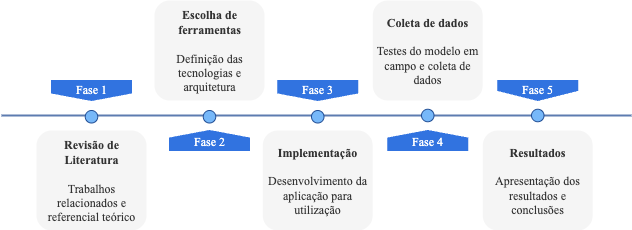
\includegraphics[width=\textwidth]{images/fases_pesquisa.png}
		\fonte{Elaborado pelo autor}
	\end{minipage}
\end{figure}
\FloatBarrier

\subsection{Proposta de Solução}

Conforme mencionado anteriormente, observa-se que o impacto da Inteligência Artificial no desenvolvimento de \textit{software} ainda é um tema em debate, sendo comum que as análises existentes se restrinjam a relatos de uso ou percepções subjetivas por parte dos desenvolvedores. Em muitos casos, a avaliação da influência da IA sobre fatores como produtividade e tempo de execução de tarefas ocorre de forma fragmentada, sem um método padronizado que permita mensurar de maneira objetiva os efeitos reais de tais ferramentas.

Dentro desse cenário, a proposta do estudo surge com a elaboração do um desafio técnico, disponibilizado através da plataforma \textit{web} desenvolvida especificamente para este fim. A ferramenta funcionou como um ambiente de avaliação controlado, no qual os participantes foram previamente organizados em dois grupos: um grupo com autorização para utilizar ferramentas de IA durante a resolução do desafio e outro grupo para realizar a atividade sem recorrer a tais recursos.

A proposta buscou, assim, criar condições equivalentes para ambos os grupos, garantindo que todos recebessem o mesmo enunciado do desafio, apresentado diretamente na plataforma. Para cada participante foi disponibilizado um \textit{link} único, correspondente ao grupo ao qual pertencia. A partir desse acesso, o desenvolvedor pôde visualizar as instruções, iniciar a tarefa e, ao concluir, submeter os arquivos com sua solução.

A plataforma também atuou como mecanismo de registro, armazenando automaticamente o tempo total gasto por cada participante, desde o momento em que deu início ao desafio até a finalização da entrega. Dessa forma, além da coleta da solução proposta, foi possível analisar métricas objetivas como tempo de conclusão, resolução dos problemas propostos (\textit{bugs}) e até mesmo, eventuais diferenças de abordagem entre os grupos.

\section{Modelo Proposto}

Esta seção tem como objetivo descrever brevemente a ferramenta desenvolvida e utilizada para a execução deste trabalho, incluindo sua arquitetura, funcionalidades e tecnologias utilizadas. O modelo proposto consiste em uma aplicação \textit{web} que centraliza as informações do desafio técnico, disponibilizando-o de forma prática e organizada para os desenvolvedores participantes do estudo.

A aplicação coleta o nome e o cargo atual do participante no mercado de trabalho. O nome é utilizado exclusivamente para exibir uma mensagem personalizada de boas-vindas. Funciona como um identificador simples durante a sessão, mantendo o usuário ativo no desafio, sem necessidade de cadastro, \textit{tokens} ou \textit{logins} complexos. Dessa forma, os nomes dos participantes não são utilizados na apresentação dos resultados do estudo, garantindo anonimato e simplicidade na utilização da ferramenta.

\subsection{Visão Geral}

A plataforma desenvolvida tem como objetivo oferecer um ambiente controlado, acessível e intuitivo para a realização de um desafio técnico. Sua concepção visa permitir a comparação entre dois grupos de participantes, um autorizado a utilizar ferramentas de IA Generativa e outro sem esse recurso, garantindo condições iguais de execução e coleta precisa de dados para análise posterior.

A aplicação dispõe de duas telas de cadastro semelhantes, diferenciadas apenas pelo tipo de participante. Uma é destinada aos desenvolvedores do grupo sem IA, e a outra aos do grupo com IA. Essa distinção é registrada internamente no banco de dados, identificando a qual grupo o participante pertence. A partir desse ponto, todo o fluxo de utilização da plataforma é idêntico para ambos os grupos, assegurando que todos recebam o mesmo desafio técnico, com os mesmos detalhes e informações.

Um aspecto essencial considerado durante o desenvolvimento foi o registro automático do tempo total de execução de cada participante. Esse recurso elimina a necessidade de solicitar uma estimativa manual de tempo após a conclusão, o que poderia gerar dados imprecisos e subjetivos. Assim, o sistema contabiliza precisamente o período compreendido entre o momento em que o participante inicia o desafio e o instante em que o finaliza.

Além disso, a plataforma foi projetada para proporcionar uma experiência simples e direta tanto para o acesso ao código-fonte do desafio quanto para o envio da solução desenvolvida. Ao término da atividade, o sistema disponibiliza um botão que direciona o participante ao formulário de \textit{feedback}, ajustado conforme o grupo ao qual pertence (sem ou com IA). Essa diferenciação se faz necessária, pois embora algumas perguntas sejam comuns entre os grupos, outras foram elaboradas especificamente para compreender a experiência de poder, ou não, utilizar ferramentas de IA Generativa durante a execução do desafio.

\subsection{Arquitetura e Tecnologias}

A plataforma é dividida em três partes: a aplicação \textit{web}, uma \textit{API REST} e um banco de dados. A aplicação \textit{web} é responsável pelo formulário inicial (cadastro e identificação) dos desenvolvedores, exibição dos detalhes do desafio técnico e por todo o fluxo de etapas ao longo do experimento, como início do desafio, envio do arquivo com a solução por parte do desenvolvedor e finalização do desafio.

A \textit{API REST} é responsável por controlar toda a comunicação com o banco de dados do sistema, através das rotas configuradas que realizam operações como: registrar no banco de dados o tempo de ínicio do desenvolvedor (\textit{timestamp}) ao iniciar o desafio, registrar o tempo de término, armazenar o tempo total em milissegundos (ms) para a conclusão do desafio, armazenar o tipo do grupo do grupo do desenvolvedor (com ou sem IA), cargo do mesmo, realizar o download da pasta \textit{.zip} do código-fonte na máquina do participante, assim como realizar o \textit{upload} da solução do mesmo para o \textit{back-end}.

Sobre as tecnologias utilizadas, a aplicação \textit{web} foi desenvolvida utilizando \textit{React.js}\footnote{\textit{React.js}: \url{https://pt-br.reactjs.or}}. Esta biblioteca foi escolhida por ser bastante similar e utilizar \textit{JavaScript} como base, simplificando assim a construção da plataforma, até mesmo pela sua praticidade para a organização de páginas e componentes reutilizáveis entre elas, o que facilita muito a organização durante o desenvolvimento. Para otimizar a construção do \textit{front-end}, foi utilizado também a biblioteca \textit{Material UI}\footnote{\textit{Material UI}: \url{https://mui.com/material-ui/}}, uma biblioteca de componentes \textit{React}, \textit{open source}, que implementa o \textit{Material Design} do \textit{Google}.

Através das escolhas anteriores, acabou sendo determinante para que a \textit{API REST} fosse construída utilizando \textit{Express.js}\footnote{\textit{Express.js}: \url{https://expressjs.com/}}, sendo este um \textit{framework} minimalista e flexível para \textit{Node.js}\footnote{\textit{Node.js}: \url{https://nodejs.org/pt}}, que simplifica consideravelmente a criação de \textit{APIs}, fornecendo ferramentas para tarefas como roteamento e manipulação de requisições \textit{HTTP}. Além de prático com sua leveza e liberdade oferecida durante o processo de desenvolvimento, resultam em conseguir realizar a entrega de uma solução simples com mais precisão.

Por fim, a transferência de dados entre a aplicação web com a \textit{API} foi feita utilizando arquivos \textit{JSON}, recebendo-os e manipulando-os. Para o banco de dados, foi utilizado \textit{PostgreSQL}\footnote{\textit{PostgreSQL}: \url{https://www.postgresql.org/}}, por ser um banco de dados relacional de objeto e \textit{open source}, conhecido por sua robustez, confiabildade, extensibilidade e até mesmo, fácil manuseio e implementação. Ele suporta tanto dados relacionais (\textit{SQL}) quanto não relacionais (\textit{JSON}), compatibilidade com padrões \textit{SQL}, e funcionalidades avançadas como chaves estrangeiras, gatilhos e recuperação pontual. Por ser \textit{open soruce}, o \textit{PostgreSQL} é igualmente gratuito. Para a estrutura das tabelas e seus dados, foi seguido o modelo de dados relacionais (\textit{SQL}), afinal, foram necessárias somente três tabelas para o banco de dados, sendo elas:

\begin{itemize}[leftmargin=1cm, itemsep=0.1em, topsep=0.1em]
    \item \textit{Developer}, responsável por armazenar as informações do administrador e dos participantes;
    \item \textit{Challenge}, responsável por armazenar os dados de início, término e tempo total da conclusão do desafio de cada participante;
    \item \textit{DeveloperChallenge}, responsável por armazenar os dados referentes ao arquivo de solução do desenvolvedor.
\end{itemize}

O diagrama ER do banco de dados está disponível no Apêndice A. Sobre o \textit{deploy} de todas as camadas da plataforma, a aplicação \textit{web} foi hospedada na plataforma \textit{Vercel}\footnote{\textit{Vercel}: \url{ https://vercel.com/}}, que possui planos gratuitos e também pela  praticidade de sua integração ao repositório no \textit{GitHub}\footnote{\textit{GitHub}: \url{https://github.com/}}, que facilita no processo de \textit{deploys} automáticos conforme novos \textit{commits} vão sendo feitos ao repositório remoto.

Por fim, a \textit{API} e o banco de dados \textit{PostgreSQL} foram hospedados na plataforma \textit{Railway}\footnote{\textit{Railway}: \url{https://railway.com/}}, por possuir planos com créditos limitados para consumo/uso por alguns dias ou até o término dos créditos. Sua versatilidade para igualmente integrar ao repositório no \textit{GitHub}, também trouxe praticidade para que o \textit{deploy} da \textit{API} fosse realizado sem muitas complicações a cada novo \textit{commit}. Para o banco de dados, foi exportado somente o arquivo \texttt{.dump} do ambiente local de desenvolviemnto e importado para o \textit{Railway}.

As ferramentas utilizadas no processo de desenvolvimento foram o \textit{Visual Studio Code}\footnote{\textit{Visual Studio Code}: \url{https://code.visualstudio.com/}} (\textit{VS Code}), editor de código-fonte popularmente conhecido, especialmente para o desenvolvimento de aplicações \textit{web} e praticidade para o uso do \textit{terminal} dentro do \textit{VS Code}. Outra ferramenta utilizada para os testes das rotas da \textit{API} a medida em que iam sendo criadas, antes de serem integradas ao \textit{front-end}, foi a ferramenta \textit{Postman}\footnote{\textit{Postman}: \url{https://www.postman.com/}}, por facilitar a criação, testes e documentação de \textit{APIs}, permitindo o envio de requisições \textit{HTTP}/\textit{HTTPS}. Com sua interface intuitiva, se tornou prático o acompanhamento das requisições que eram feitas e a armazenagem dos dados no banco.

Um breve diagrama da arquitetura do modelo é ilustrado na Figura \ref{fig:arquitetura}.

\begin{figure}[ht]
    \caption{Arquitetura do modelo}
    \label{fig:arquitetura}
    \centering
    \footnotesize
    \begin{minipage}{.9\textwidth}
        \centering
        \fbox{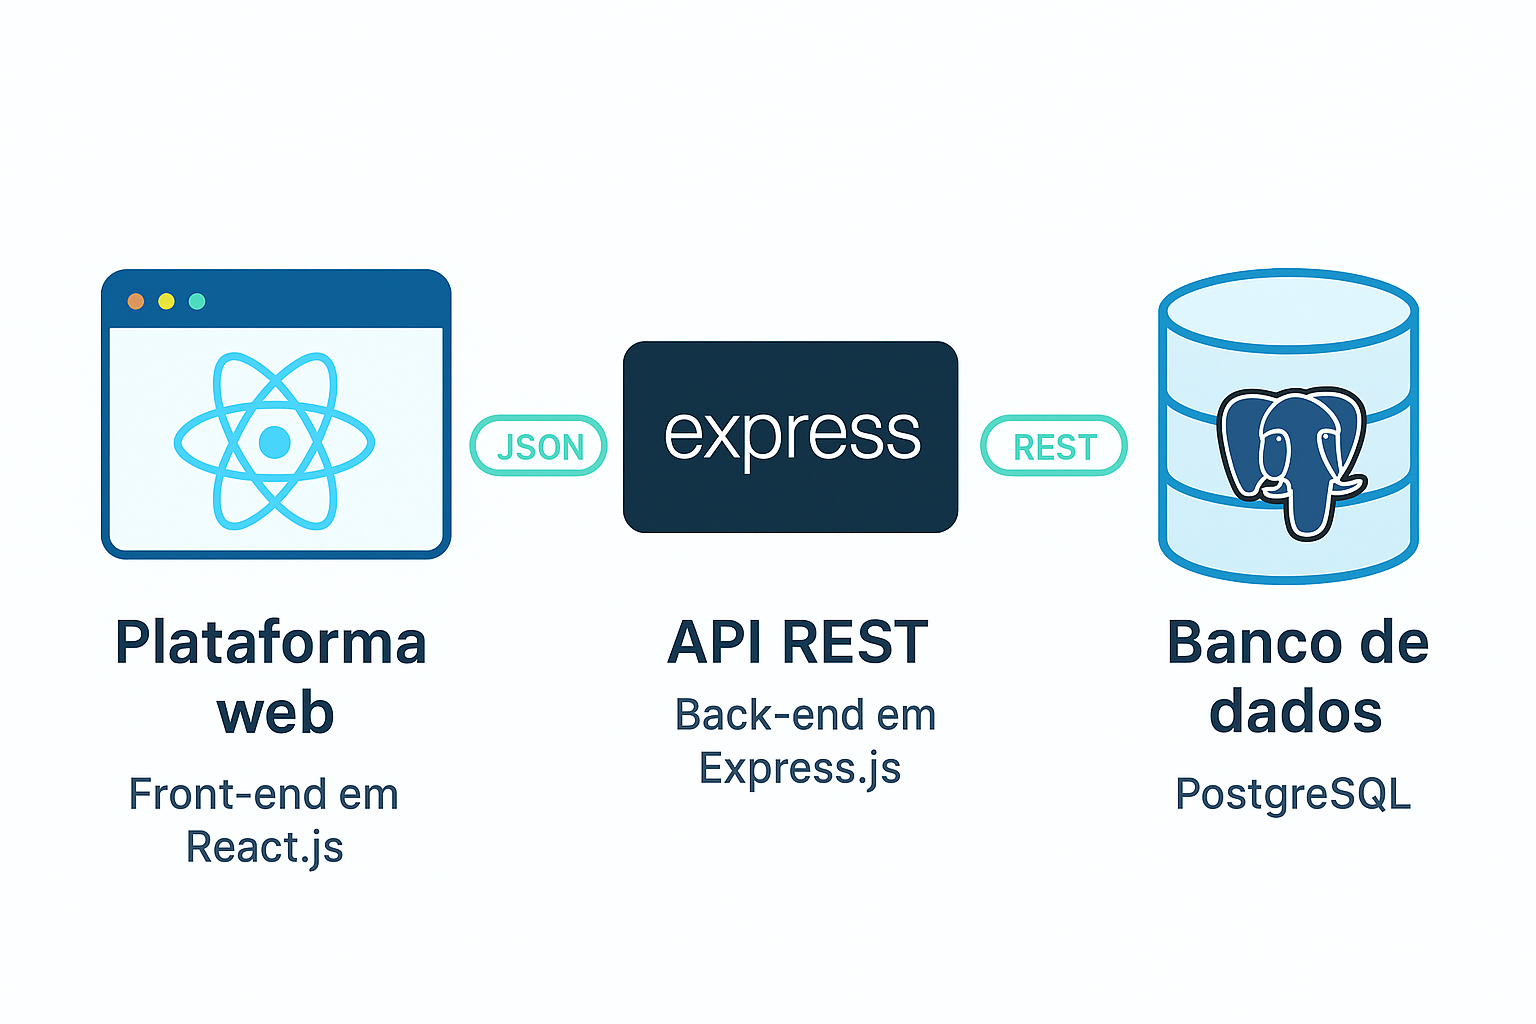
\includegraphics[width=0.50\textwidth]{images/arquitetura.png}}
        \fonte{Elaborado pelo autor}
    \end{minipage}
\end{figure}
\FloatBarrier

\subsection{Funcionalidades}

A seguir serão apresentadas as principais funcionalidades da plataforma proposta para o desenvolvimento deste modelo, detalhando cada um delas. Nesta seção estão as telas dos fluxos  de uso e etapas dentro da plataforma. As demais telas estão disponíveis no Apêndice B.

\subsection{Formulário Inicial}

Ao acessar a plataforma \textit{web} através do \textit{link} fornecido juntamente com as instruções iniciais via \textit{WhatsApp} para cada participante, o desenvolvedor necessita preencher um breve formulário informando seu "Nome e Sobrenome" (que é somente de uso interno na plataforma), seu "Cargo atual" e então pressionar o botão "Registrar". Os campos "Nome e Sobrenome" e "Cargo atual" são obrigatórios para o participante poder avançar. Nas Figuras \ref{fig:cadastro_sem_ia} e \ref{fig:cadastro_com_ia} estão as telas de registro dos participantes do grupo sem IA e com IA, respectivamente.

\begin{figure}[ht]
    \caption{Cadastro do participante do grupo sem IA}
    \label{fig:cadastro_sem_ia}
    \centering
    \footnotesize
    \begin{minipage}{.9\textwidth}
        \centering
        \fbox{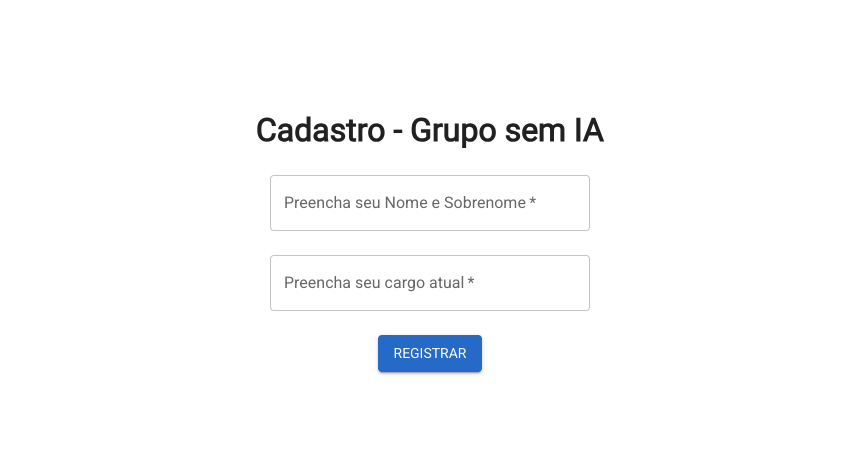
\includegraphics[width=0.65\textwidth]{images/cadastro_sem_ia.png}}
        \fonte{Elaborado pelo autor}
    \end{minipage}
\end{figure}
\FloatBarrier

\begin{figure}[ht]
    \caption{Cadastro do participante do grupo com IA}
    \label{fig:cadastro_com_ia}
    \centering
    \footnotesize
    \begin{minipage}{.9\textwidth}
        \centering
        \fbox{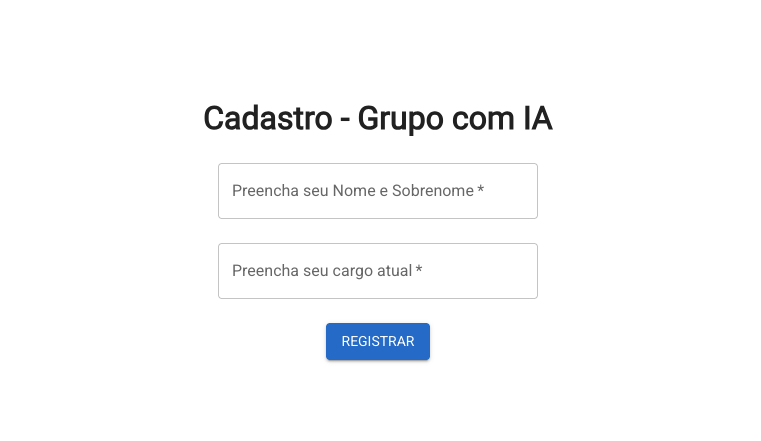
\includegraphics[width=0.65\textwidth]{images/cadastro_com_ia.png}}
        \fonte{Elaborado pelo autor}
    \end{minipage}
\end{figure}
\FloatBarrier

\subsection{Tela Inicial e Informações do Desafio}

Após o preenchimento do formulário inicial, o participante é direcionado para a primeira tela da plataforma, que neste caso é a tela do desafio técnico propriamente. Porém, nesta tela, antes de exibir os detalhes do desafio, é exibido mais algumas informações que reforçam a necessidade de atenção e dedicação do participante antes de dar início ao teste. 

Estando de acordo, o participante clica no botão "De acordo" e na mesma tela é renderizada todos os detalhes e imagens de cenários de exemplo, descrevendo o desafio técnico que o desenvolvedor irá solucionar. A tela inicial e as informações do desafio encontram-se na Figura \ref{fig:tela_inicial} e \ref{fig:informacoes_desafio}, respectivamente.

\begin{figure}[ht]
    \caption{Tela inicial}
    \label{fig:tela_inicial}
    \centering
    \footnotesize
    \begin{minipage}{.9\textwidth}
        \centering
        \fbox{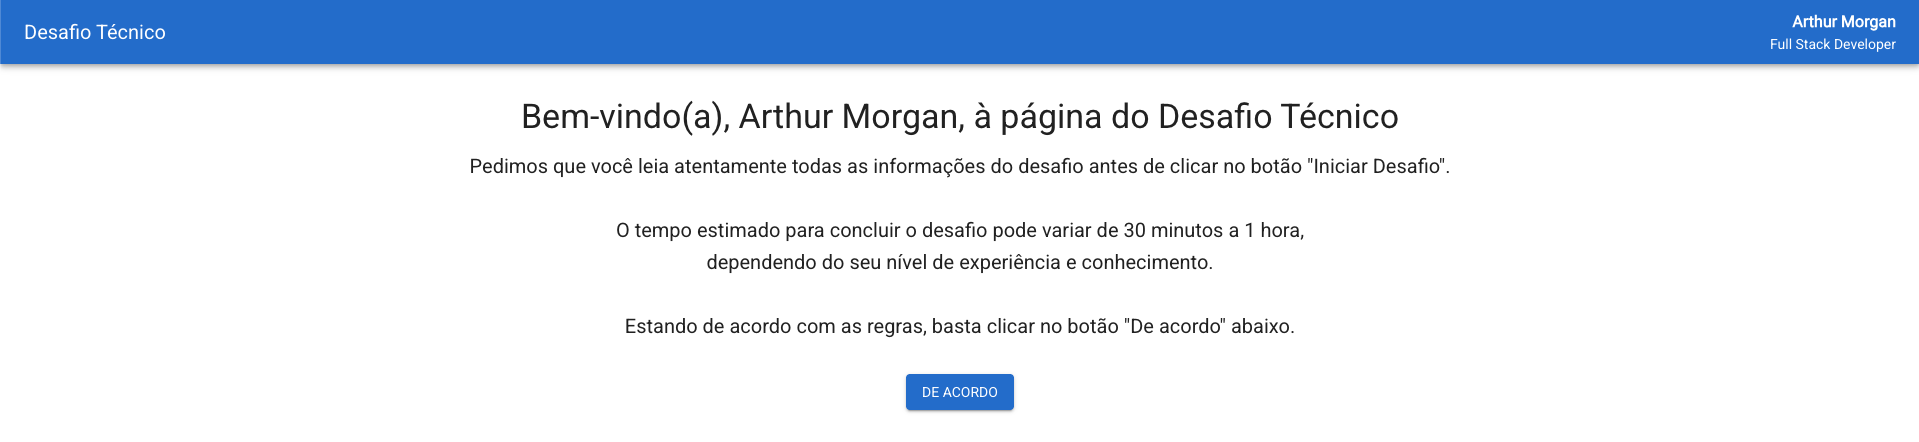
\includegraphics[width=0.95\textwidth]{images/tela_inicial.png}}
        \fonte{Elaborado pelo autor}
    \end{minipage}
\end{figure}
\FloatBarrier

\begin{figure}[ht]
    \caption{Informações do desafio}
    \label{fig:informacoes_desafio}
    \centering
    \footnotesize
    \begin{minipage}{.9\textwidth}
        \centering
        \fbox{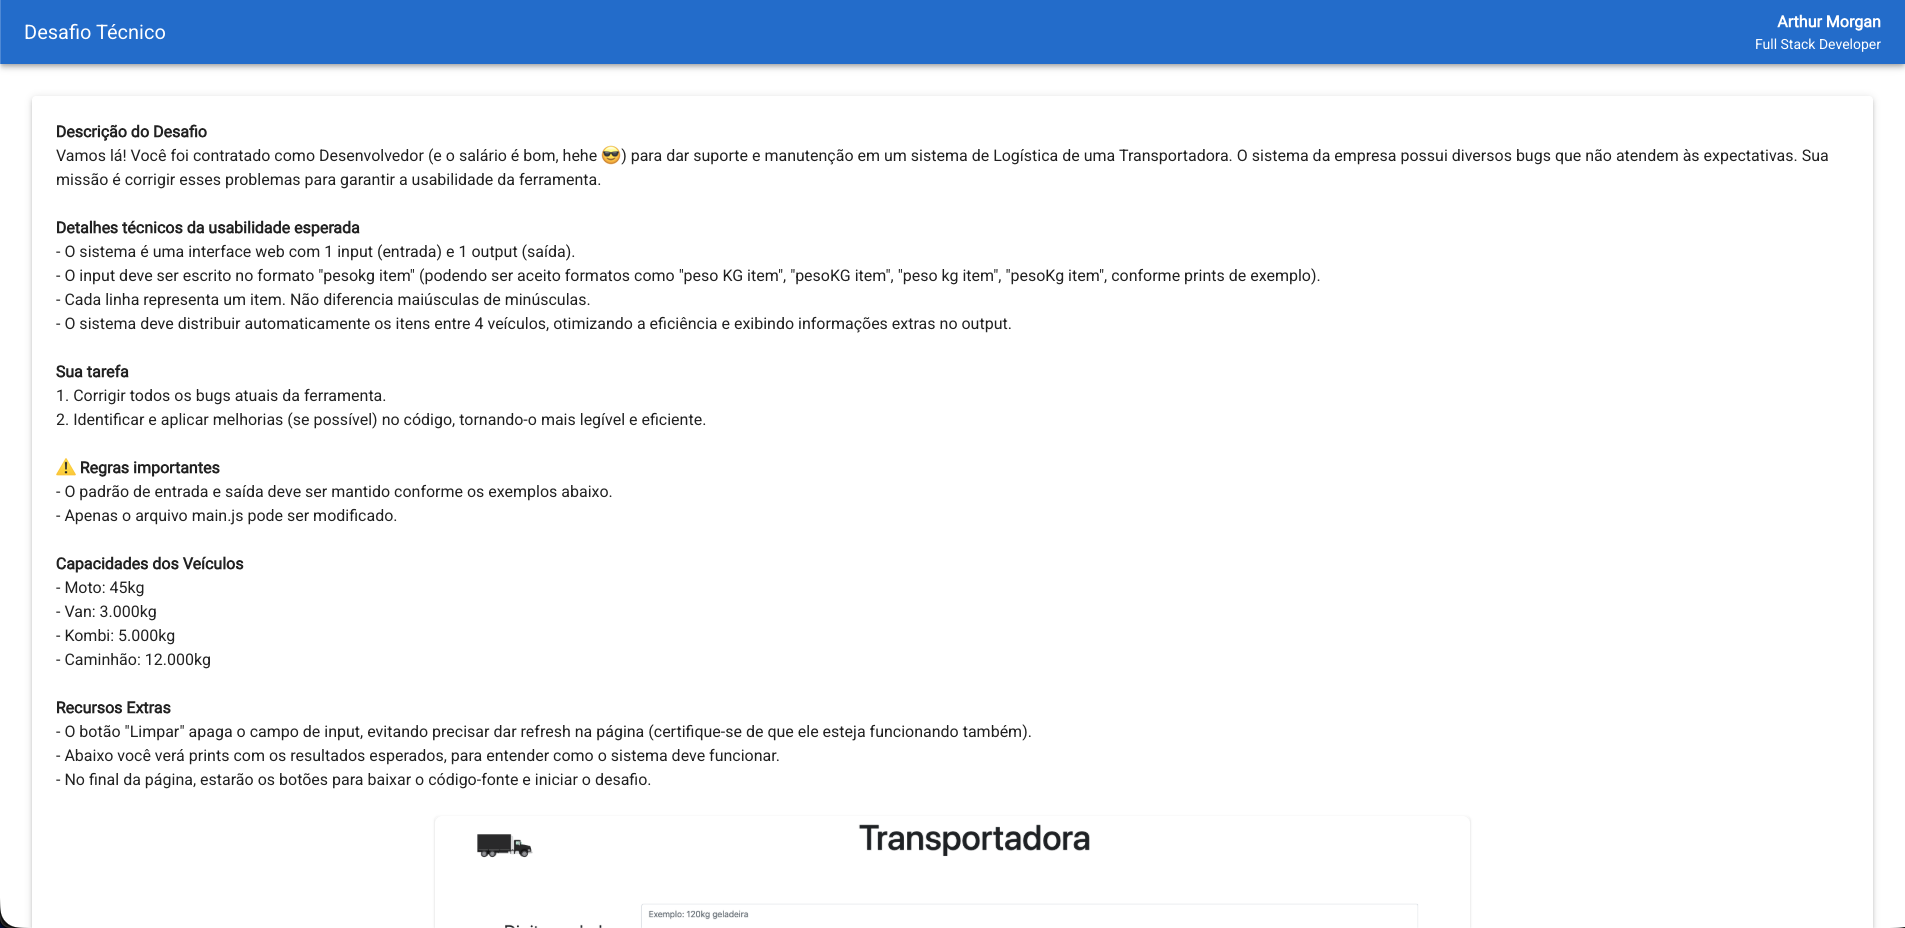
\includegraphics[width=0.95\textwidth]{images/informacoes_desafio.png}}
        \fonte{Elaborado pelo autor}
    \end{minipage}
\end{figure}
\FloatBarrier

Ao descer um pouco a tela, o desenvolvedor encontra as imagens de cenários de exemplo que ilustram o objetivo final das funcionalidades que a solução precisa atender para concluir o desafio de modo satisfatório, como exemplo da Figura \ref{fig:exemplos_desafio}.

\begin{figure}[ht]
    \caption{Cenário de exemplo}
    \label{fig:exemplos_desafio}
    \centering
    \footnotesize
    \begin{minipage}{.9\textwidth}
        \centering
        \fbox{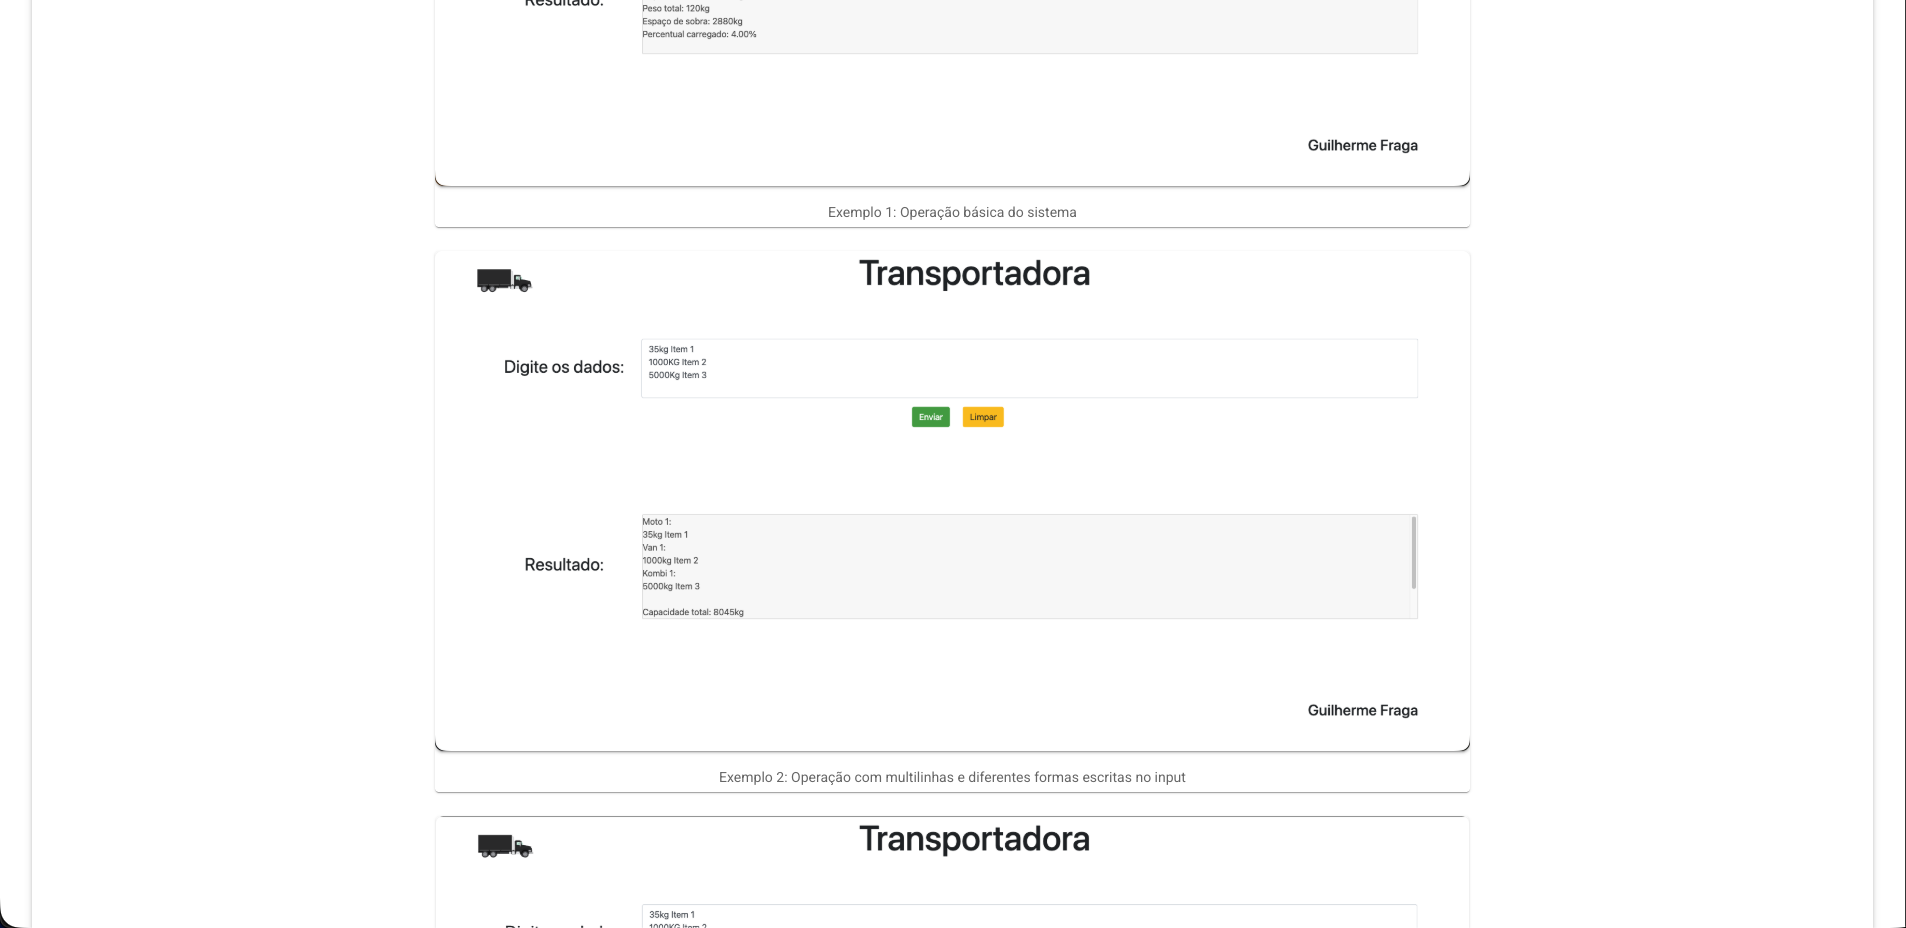
\includegraphics[width=0.95\textwidth]{images/exemplos_desafio.png}}
        \fonte{Elaborado pelo autor}
    \end{minipage}
\end{figure}
\FloatBarrier

Ao final da tela, conforme a Figura \ref{fig:baixar_iniciar_desafio}, está o botão para realizar o \textit{download} do código-fonte do desafio técnico e logo abaixo, o botão para iniciar o desafio, que só é habilitado após o participante acionar o anterior, ou seja, realizar o \textit{download}. Nesta parte também foi colocado mais um aviso reforçando a importância do participante preparar seu ambiente de desenvolvimento antes de clicar em "iniciar desafio", pois ao acionar este botão, uma rota da \textit{API} é chamada que armazena no banco de dados o horário de início (\textit{timestamp}) do desenvolvedor, registrando assim o momento exato em que o participante iniciou a atividade.

\begin{figure}[ht]
    \caption{Baixar e iniciar desafio}
    \label{fig:baixar_iniciar_desafio}
    \centering
    \footnotesize
    \begin{minipage}{.9\textwidth}
        \centering
        \fbox{
\includegraphics[width=0.95\textwidth]{images/baixar_iniciar_desafio.png}}
        \fonte{Elaborado pelo autor}
    \end{minipage}
\end{figure}
\FloatBarrier

\subsection{Desafio Técnico}

Para o desenvolvimento do desafio técnico proposto na plataforma, foi concebido um cenário fictício com base em um projeto particular previamente desenvolvido pelo pesquisador, utilizado anteriormente apenas para fins de estudo pessoal. Esse projeto consiste em um sistema simples de logística de uma transportadora, composto por uma interface \textit{web} básica que recebe um \textit{input} e retorna um \textit{output} correspondente.

Os dados de \textit{input} representam itens no formato “pesokg item” (também aceitando variações como “peso KG item” ou “peso kg item”), nos quais o sistema deve distribuir automaticamente cada item entre os tipos de veículos disponíveis, conforme suas respectivas capacidades. O objetivo é otimizar a alocação dos itens e apresentar, no \textit{output}, os detalhes dessa distribuição.

Cada linha do campo de \textit{input} representa um item, sem distinção entre letras maiúsculas e minúsculas. O sistema contempla quatro tipos de veículos, cada um com uma capacidade específica. Em determinadas simulações, mais de um veículo do mesmo tipo pode ser utilizado quando os itens se encaixam nessa categoria. Por exemplo, para dois itens de 45 kg, seriam alocadas duas motos, pois cada uma suporta até 45 kg.

Para o desafio técnico, foi fornecido todo o código-fonte do sistema, incluindo os arquivos \texttt{index.html} e \texttt{style.css}, responsáveis pela interface \textit{web}. Entretanto, como regra, os participantes deveriam modificar apenas o arquivo \texttt{main.js}, que contém toda a lógica de negócio do sistema de logística. Dessa forma, poderiam realizar os testes diretamente na interface \textit{web} já pronta, sem necessidade de ajustes adicionais.

Com base no código-fonte funcional (disponível integralmente no Apêndice G), foram inseridos diversos \textit{bugs} propositais no arquivo \texttt{main.js} (cuja versão modificada também se encontra disponível neste mesmo Apêndice) fragmentando o código em diferentes pontos para que os participantes os identificassem e corrigissem. Esses \textit{bugs} foram organizados em uma lista para controle e análise posterior, conforme apresentado no Apêndice H.

\subsection{Tela de \textit{Upload}}

Após o participante clicar no botão "Iniciar Desafio", o mesmo é direcionado para a tela de \textit{upload}. Nesta tela, as informações referentes ao desafio permanecem sem alterações, para que fosse possível ao participante consultar a medida que fosse solucionando os \textit{bugs}. O diferencial desta tela se dá pelo título no topo, conforme a Figura \ref{fig:tela_upload}, indicando ao participante que ao término da sua solução, o mesmo deve descer até o final da página para realizar o envio do seu arquivo através dos botões indicados. 

\begin{figure}[ht]
    \caption{Tela de \textit{Upload}}
    \label{fig:tela_upload}
    \centering
    \footnotesize
    \begin{minipage}{.9\textwidth}
        \centering
        \fbox{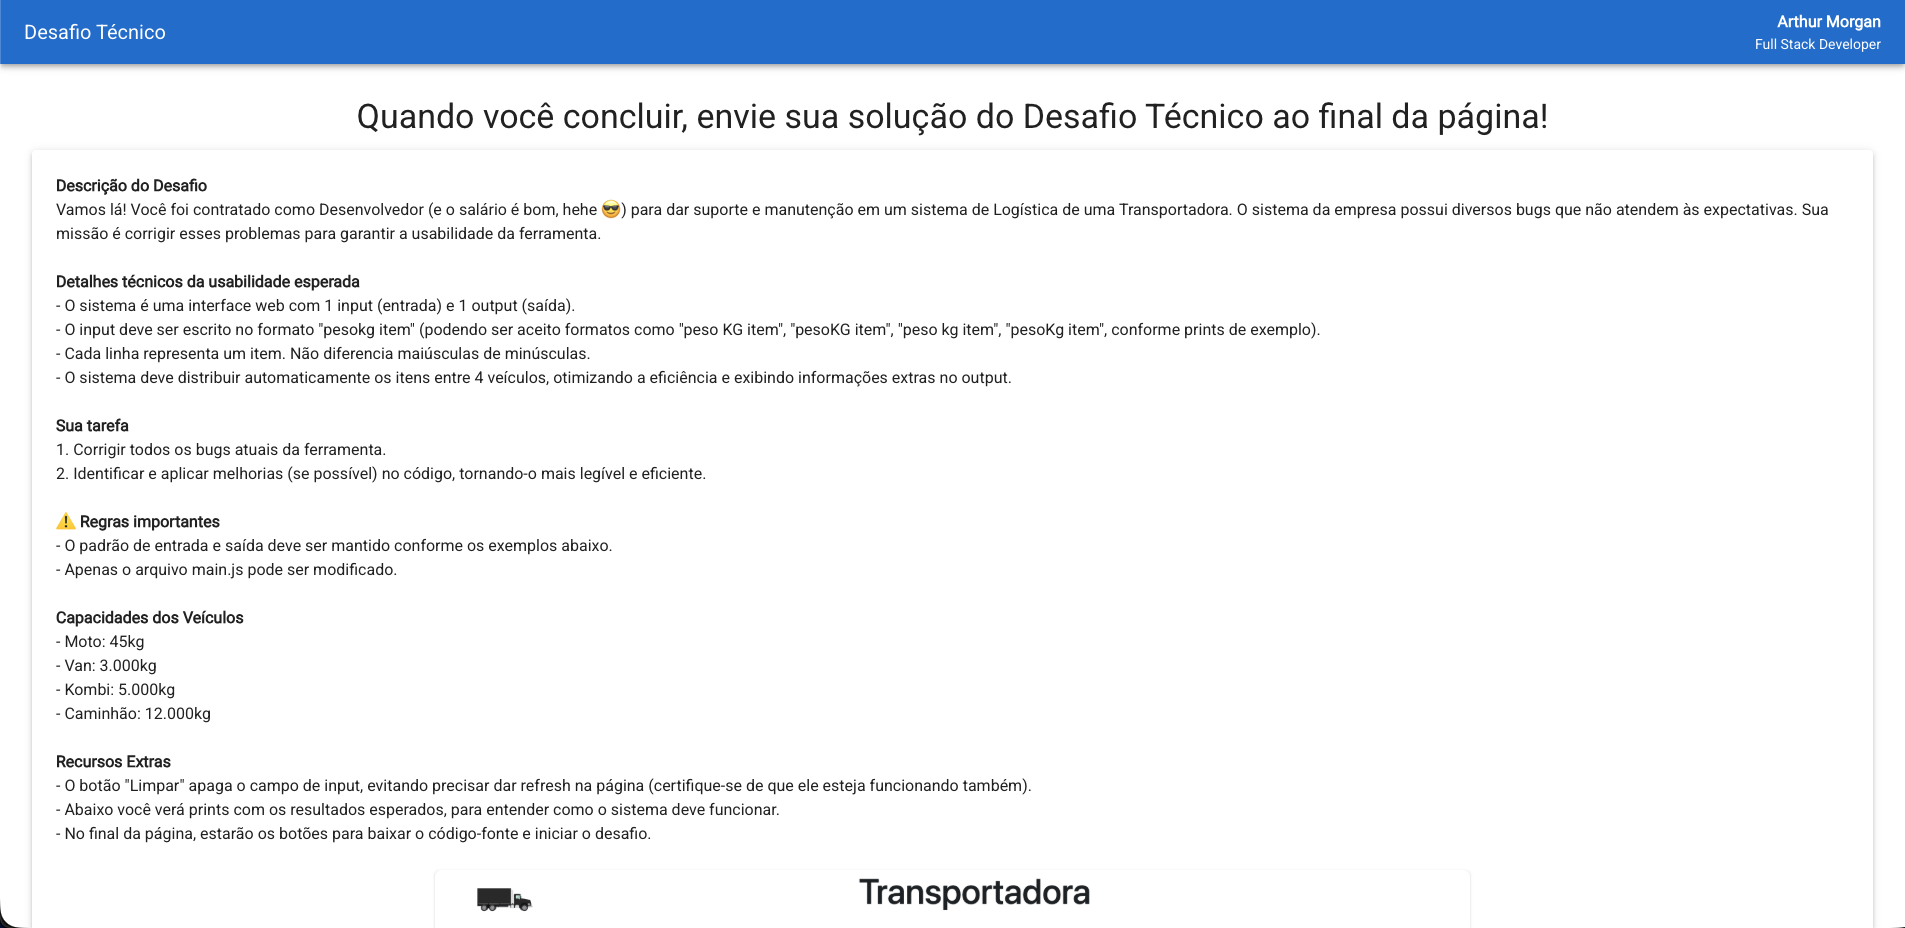
\includegraphics[width=0.95\textwidth]{images/tela_upload.png}}
        \fonte{Elaborado pelo autor}
    \end{minipage}
\end{figure}
\FloatBarrier

No final da página, encontram-se os botões para selecionar o arquivo e finalizar o desafio. O segundo botão é habilitado apenas após a seleção de um arquivo, podendo ser substituído posteriormente caso o participante deseje enviar outro — por exemplo, após corrigir sua solução antes da conclusão do desafio.

Para tornar o processo mais prático, a plataforma foi configurada para aceitar apenas arquivos no formato \textit{.zip}, permitindo que o desenvolvedor simplesmente compacte a pasta do projeto e realize o envio. Ao selecionar o arquivo, a aplicação o armazena temporariamente na pasta \textit{tmp} do \textit{back-end}. Quando o botão “Finalizar Desafio” é acionado, a rota da \textit{API} responsável pelo encerramento é executada, registrando no banco de dados o \textit{timestamp} de conclusão e calculando automaticamente o tempo total de execução, em milissegundos, com base na diferença entre o início e o término. Em seguida, o arquivo é movido da pasta \textit{tmp} para a pasta definitiva \textit{uploads}. A Figura \ref{fig:selecionar_arquivo_finalizar_desafio} ilustra os botões mencionados.

\begin{figure}[ht]
    \caption{Selecionar arquivo e finalizar desafio}
    \label{fig:selecionar_arquivo_finalizar_desafio}
    \centering
    \footnotesize
    \begin{minipage}{.9\textwidth}
        \centering
        \fbox{
\includegraphics[width=0.95\textwidth]{images/selecionar_arquivo_finalizar_desafio.png}}
        \fonte{Elaborado pelo autor}
    \end{minipage}
\end{figure}
\FloatBarrier

Após o desafio finalizado, o participante é direcionado para uma tela final de agradecimento, com um botão para direcioná-lo ao preenchiemnto do formulário de \textit{feedback} do experimento através da ferramenta \textit{Google Forms}\footnote{\textit{Google Forms}: \url{https://workspace.google.com/intl/pt-BR/products/forms/}}, conforme a Figura \ref{fig:tela_final_formulario} abaixo.

\begin{figure}[ht]
    \caption{Tela final e formulário}
    \label{fig:tela_final_formulario}
    \centering
    \footnotesize
    \begin{minipage}{.9\textwidth}
        \centering
        \fbox{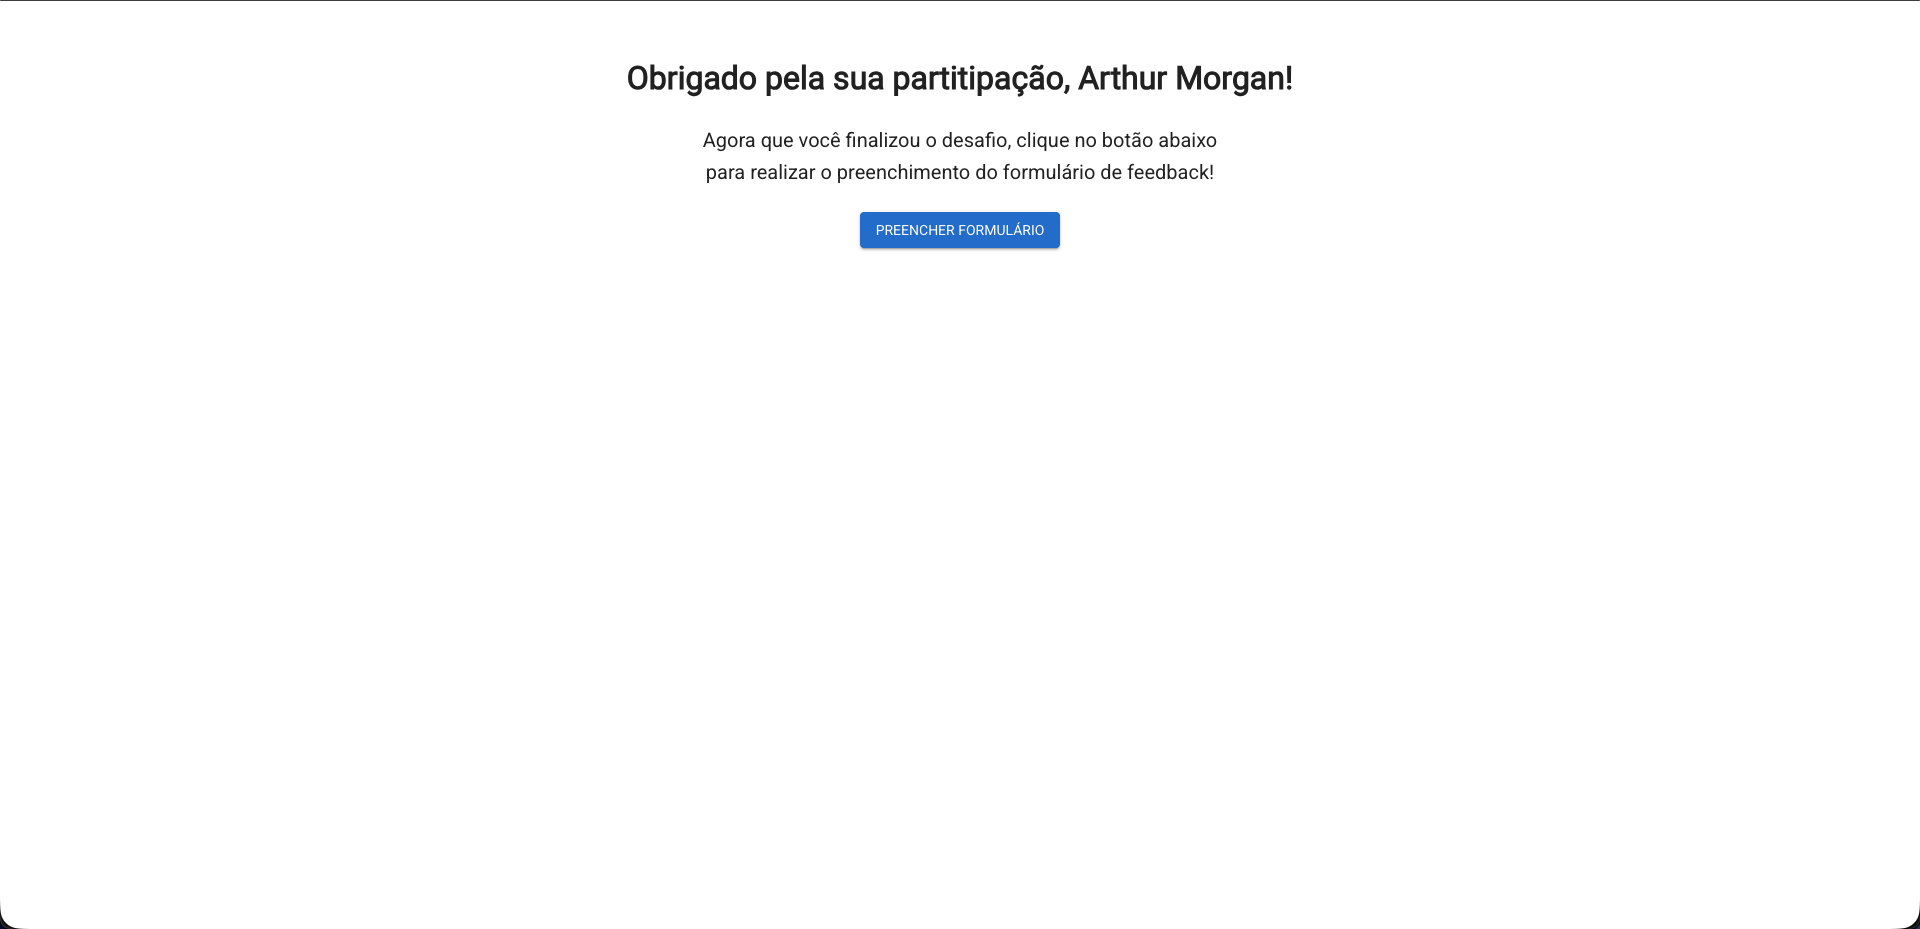
\includegraphics[width=0.95\textwidth]{images/tela_final_formulario.png}}
        \fonte{Elaborado pelo autor}
    \end{minipage}
\end{figure}
\FloatBarrier

\subsection{Painel de Administrador}

O acompanhamento das soluções dos desenvolvedores foram realizadas através de um painel de uso exclusivo do administrador do experimento. Este painel foi projetado com o objetivo de centralizar as informações principais dos participantes, agrupando-os em dados gerais e em seus grupos alocados (sem IA e com IA). O acesso deste painel é feito através de um \textit{link}\footnote{\textit{Link} para o Painel de Administrador: \url{https://ai-use-productivity.vercel.app/admin}}, que funciona como um "login" simples, apenas informando o nome do administrador, que aciona uma rota da API para validar se este nome informado está registrado no banco de dados como administrador. Esta tela encontra-se na Figura \ref{fig:painel_admin}.

\begin{figure}[ht]
    \caption{Acesso ao Painel de Administrador}
    \label{fig:painel_admin}
    \centering
    \footnotesize
    \begin{minipage}{.9\textwidth}
        \centering
        \fbox{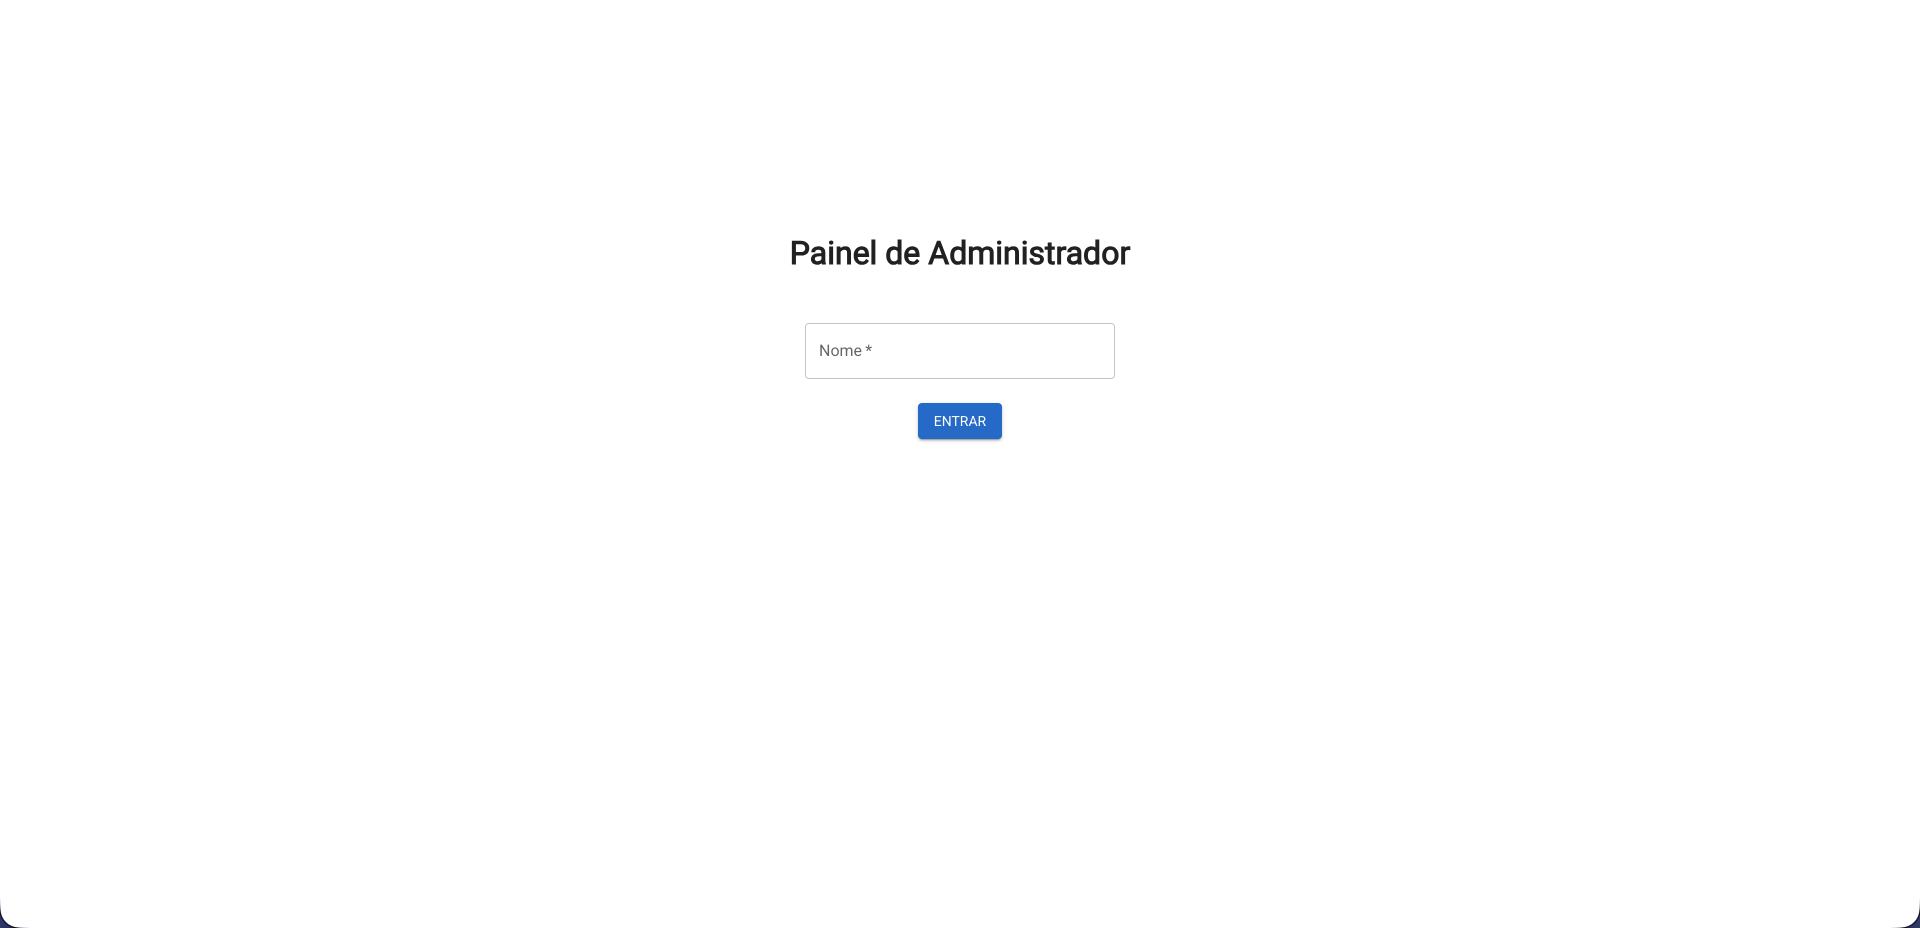
\includegraphics[width=0.65\textwidth]{images/painel_admin.png}}
        \fonte{Elaborado pelo autor}
    \end{minipage}
\end{figure}
\FloatBarrier

Acessando então como administrador, direciona-se para a tela de painel central, onde exibe informações gerais como o total de participantes do experimento, quantos pertencem ao grupo com IA, quantos pertencem ao grupo sem IA, a quantidade de arquivos enviados (soluções dos desenvolvedores) e o tempo médio geral de todos os participantes. A Figura \ref{fig:painel_central_admin} demonstra esta tela.

\begin{figure}[ht]
    \caption{Painel Central}
    \label{fig:painel_central_admin}
    \centering
    \footnotesize
    \begin{minipage}{.9\textwidth}
        \centering
        \fbox{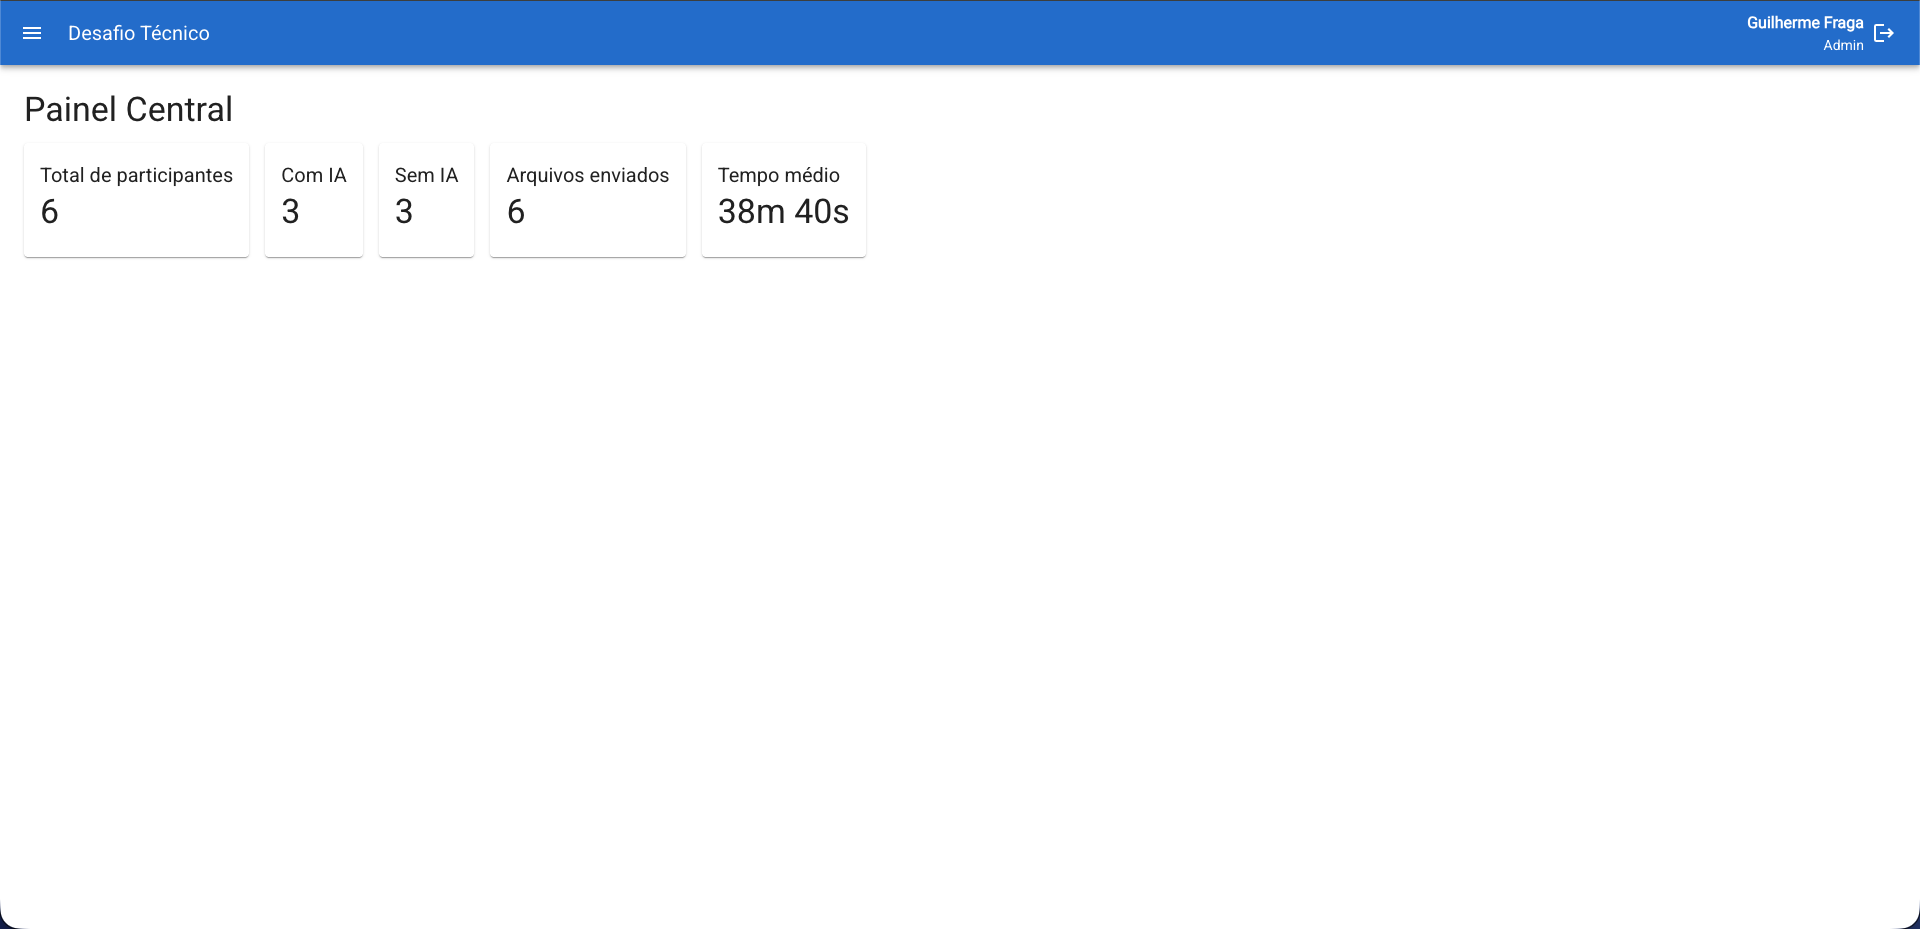
\includegraphics[width=0.95\textwidth]{images/painel_central_admin.png}}
        \fonte{Elaborado pelo autor}
    \end{minipage}
\end{figure}
\FloatBarrier

Na barra lateral esquerda, a opção “Resultados” exibe, em formato de \textit{cards}, os dados individuais de cada participante. Em cada \textit{card}, são apresentados o cargo do desenvolvedor, o tempo total gasto na conclusão do desafio, o grupo ao qual pertencia e o nome do arquivo enviado.

Para facilitar a identificação dos arquivos, o sistema aplica uma convenção automática de nomenclatura no momento do \textit{upload}, salvando-os no \textit{back-end} no formato ``\textit{id-Nome\_Sobrenome-nome\_do\_arquivo\_do\_participante.zip}``. Ao lado do nome de cada arquivo, há um botão “Baixar”, que permite realizar o \textit{download} da solução para análise posterior.

A Figura \ref{fig:resultados_gerais_admin} apresenta essa tela. Para preservar o anonimato dos participantes, as imagens exibidas no painel do administrador foram editadas para ocultar seus nomes.

\begin{figure}[ht]
    \caption{Resultados gerais}
    \label{fig:resultados_gerais_admin}
    \centering
    \footnotesize
    \begin{minipage}{.9\textwidth}
        \centering
        \fbox{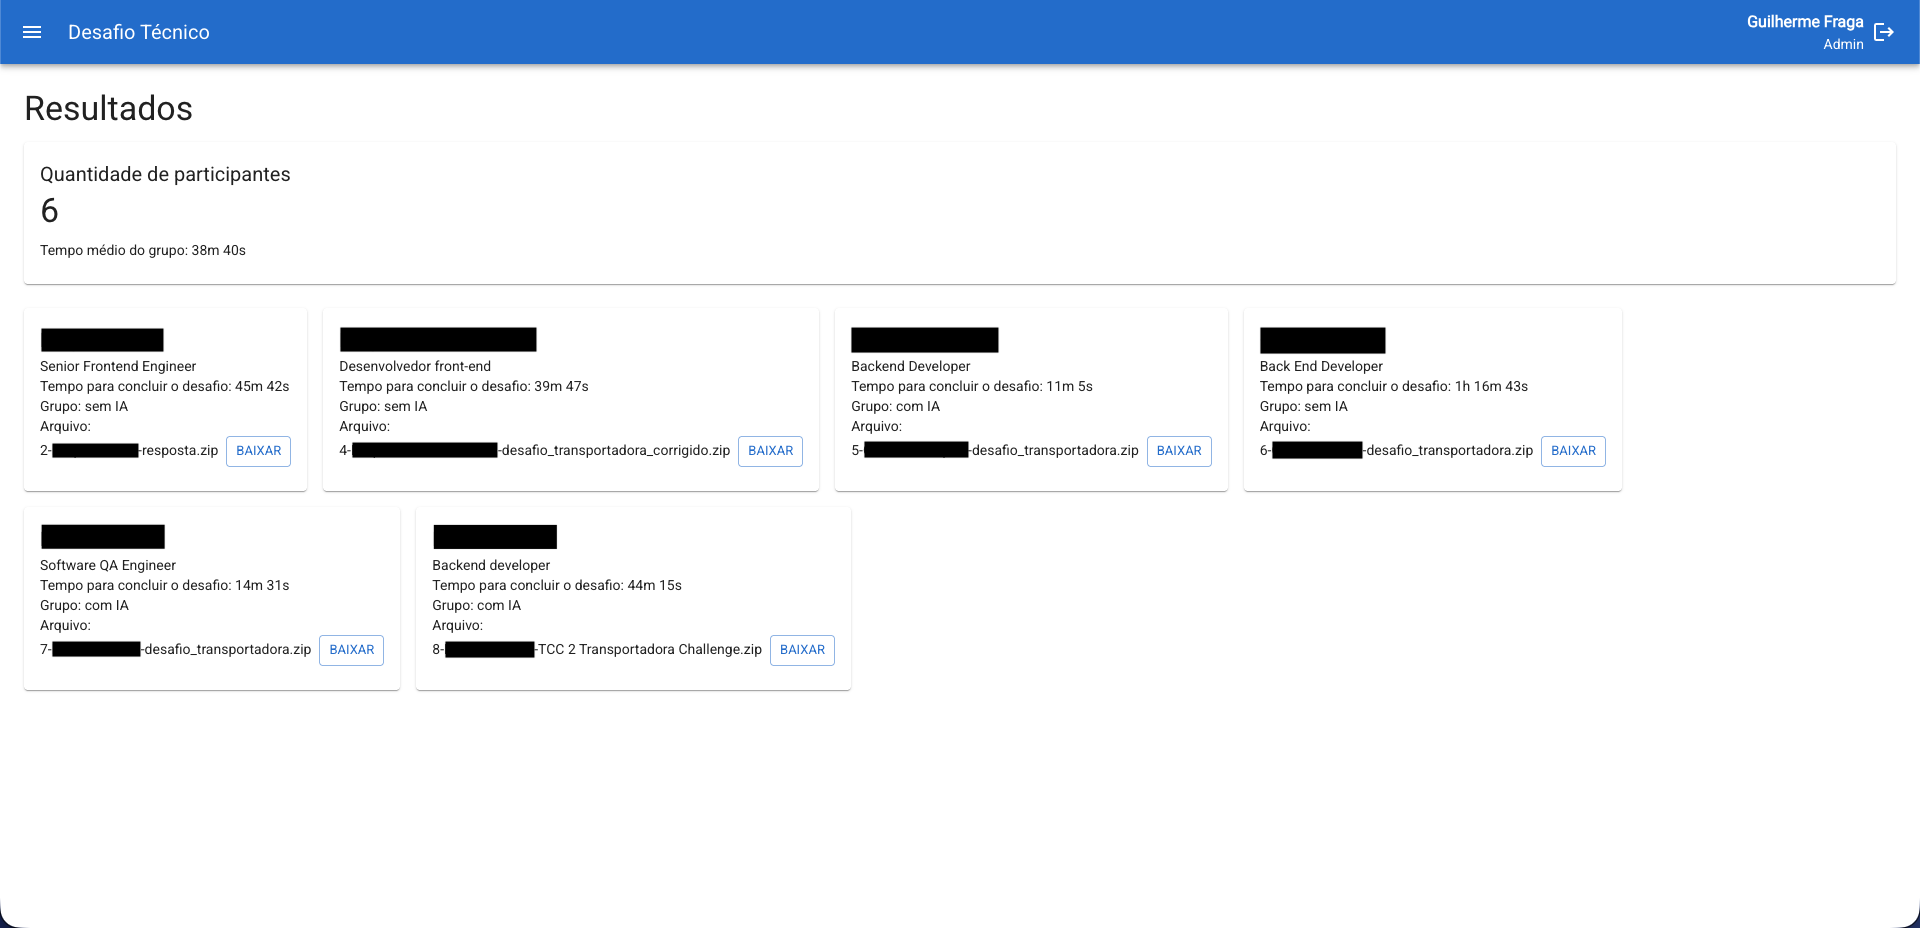
\includegraphics[width=0.95\textwidth]{images/resultados_gerais_admin.png}}
        \fonte{Elaborado pelo autor}
    \end{minipage}
\end{figure}
\FloatBarrier

As outras duas opções dos menus na barra lateral são para separar os resultados nos dois grupos, através da tela "Resultados Desenvolvedores sem IA" e "Resultados Desenvolvedores com IA". Os exemplos destas telas com os resultados do grupo sem IA e com IA, podem ser conferidos através das Figuras \ref{fig:resultados_sem_ia_admin} e \ref{fig:resultados_com_ia_admin}, respectivamente.

\begin{figure}[ht]
    \caption{Resultados Desenvolvedores sem IA}
    \label{fig:resultados_sem_ia_admin}
    \centering
    \footnotesize
    \begin{minipage}{.9\textwidth}
        \centering
        \fbox{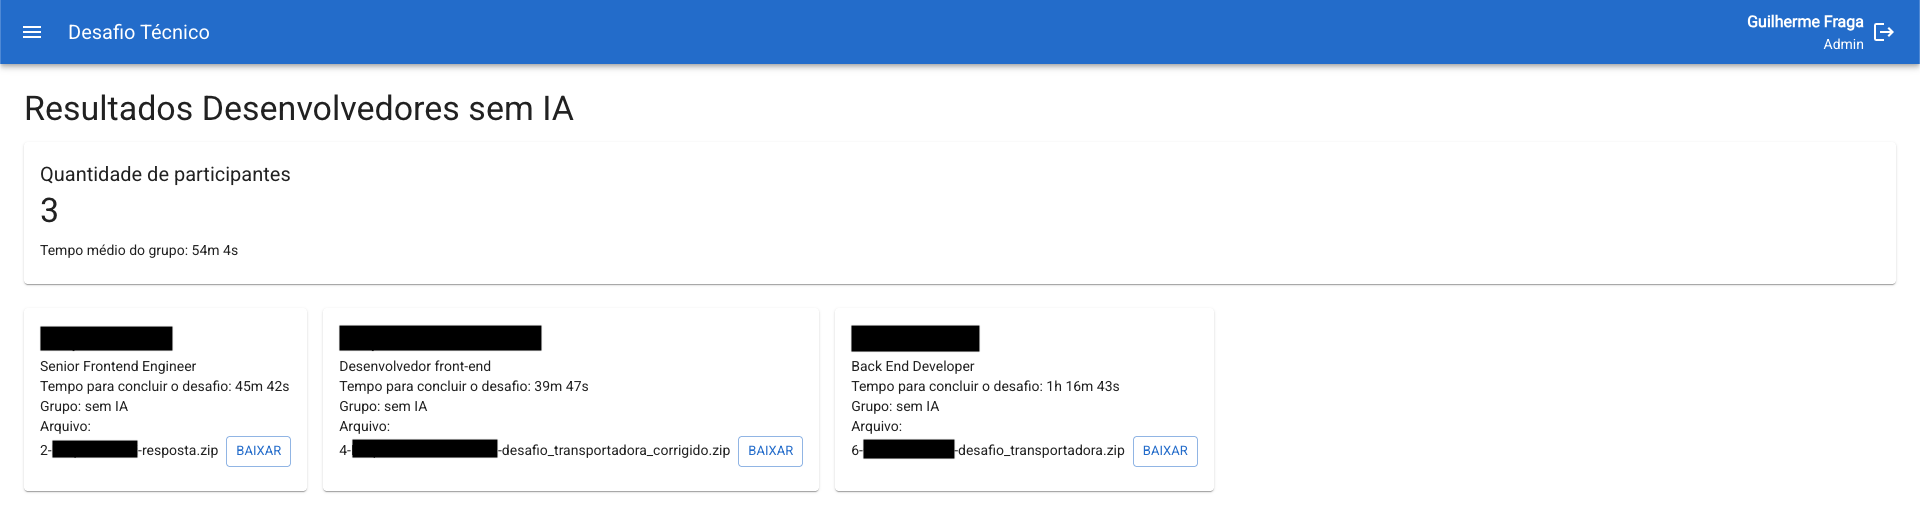
\includegraphics[width=0.95\textwidth]{images/resultados_sem_ia_admin.png}}
        \fonte{Elaborado pelo autor}
    \end{minipage}
\end{figure}
\FloatBarrier

\begin{figure}[ht]
    \caption{Resultados Desenvolvedores com IA}
    \label{fig:resultados_com_ia_admin}
    \centering
    \footnotesize
    \begin{minipage}{.9\textwidth}
        \centering
        \fbox{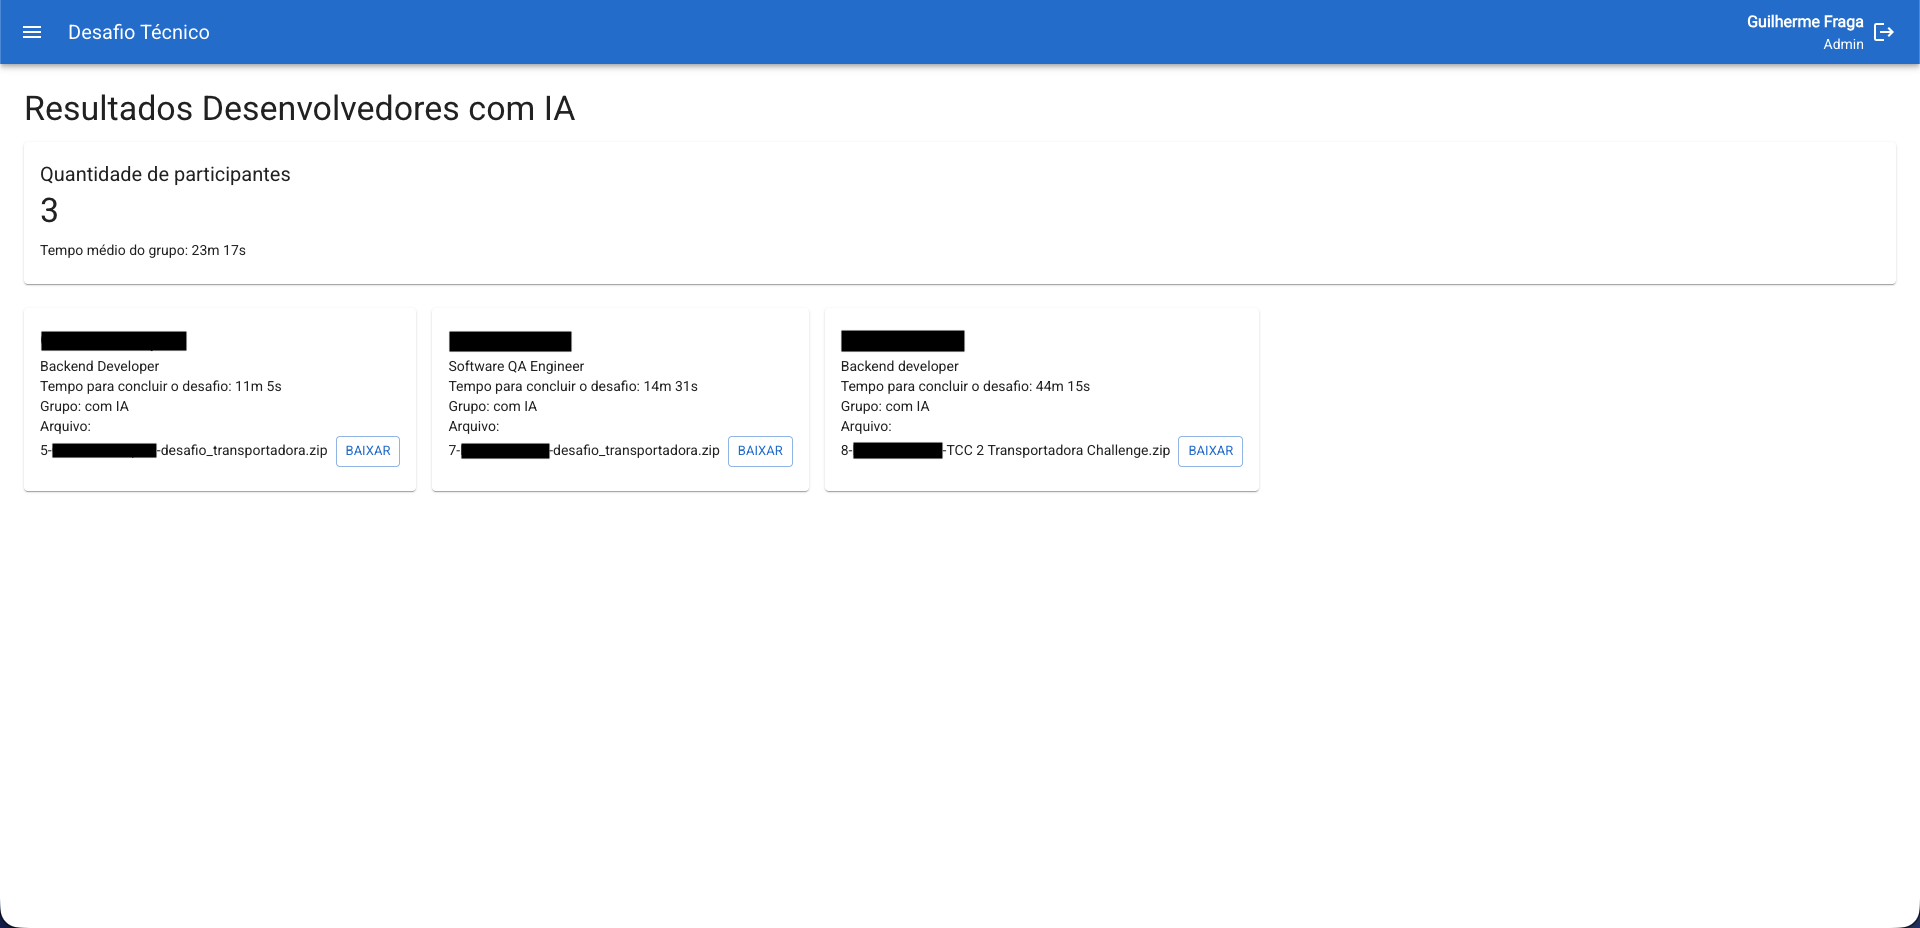
\includegraphics[width=0.95\textwidth]{images/resultados_com_ia_admin.png}}
        \fonte{Elaborado pelo autor}
    \end{minipage}
\end{figure}
\FloatBarrier

Todo o código-fonte da plataforma encontra-se disponível através do repositório\footnote{Repositório: \url{https://github.com/guifraga8/AI-Use-Productivity}} na plataforma \textit{GitHub}. Ao longo do desenvolvimento, foi utilizado o sistema de controle de versão \textit{Git}\footnote{\textit{Git}: \url{https://git-scm.com/}} para gerenciar todo o código-fonte.

\section{Análise e Discussão dos Resultados}

Nesta seção são apresentadas a coleta e análise dos dados levantados a partir das soluções fornecidas pelos participantes, juntamente com o registro do tempo total de duração para a conclusão do desafio de cada desenvolvedor. Foi coletado também dados de \textit{feedback} referente ao experimento através de um questionário aplicado no término do desafio, com o intuito de forncer mais resultados para uma análise relevante do projeto como um todo.

\subsection{Coleta de Dados}

Após a conclusão do desenvolvimento da plataforma \textit{web}, foram selecionados seis participantes por conveniência, isto é, profissionais da área de desenvolvimento de \textit{software} conhecidos pelo pesquisador e dispostos a participar do experimento. O público-alvo foi definido de modo que todos atuassem na área, porém em diferentes cargos, como desenvolvedor \textit{front-end} e \textit{back-end}.

Em seguida, realizou-se um sorteio para distribuir os participantes em dois grupos de forma justa e equilibrada: grupo sem IA (3 membros) e grupo com IA (3 membros). Cada participante recebeu, via \textit{WhatsApp}, uma mensagem individual contendo instruções, informações sobre o experimento e o respectivo \textit{link} de acesso à plataforma (\textit{link} do grupo sem IA\footnote{\textit{Link} do grupo sem IA: \url{https://ai-use-productivity.vercel.app/register/without_ai}} e \textit{link} do grupo com IA\footnote{\textit{Link} do grupo com IA: \url{https://ai-use-productivity.vercel.app/register/with_ai}}). As mensagens enviadas encontram-se no Apêndice C.

Ao término do desafio, isto é, após o envio da solução e o registro automático do tempo total de execução, cada participante respondeu a um questionário de \textit{feedback}, específico para seu grupo (\footnote{Formulário do grupo sem IA: \url{https://forms.gle/zdH8UPeheATCtQg67}} e \footnote{Formulário do grupo com IA: \url{https://forms.gle/cgqkPAs93RTPuJRH9}}). Da primeira à sétima questão, ambos os formulários continham perguntas idênticas, voltadas a avaliar o nível de conhecimento da linguagem \textit{JavaScript}, a dificuldade percebida, a clareza das instruções, o tempo demandado e o uso prévio de ferramentas de IA Generativa.

Da oitava à décima questão, o foco variou conforme o grupo. No grupo sem IA, investigaram-se as ferramentas utilizadas (não relacionadas à IA), a forma de abordagem do desafio e as dificuldades enfrentadas sem o uso de IA Generativa. No grupo com IA, as questões foram adaptadas para identificar as ferramentas de IA utilizadas, a forma como foram aplicadas e os obstáculos percebidos durante o uso dessas tecnologias.

Por fim, a décima primeira questão, comum a ambos os grupos, buscou coletar sugestões e comentários gerais sobre o experimento e a plataforma, visando aprimorar futuras aplicações semelhantes. Todas as questões estão apresentadas no Apêndice E, e suas respectivas respostas no Apêndice F.

\subsection{Avaliação dos Resultados}

A partir dos arquivos de soluções enviados pelos participantes, cada um foi analisado com base nos \textit{inputs} das imagens de exemplo disponíveis na plataforma, verificando se o \textit{output} obtido correspondia ao resultado esperado. Para isso, foram realizados testes diretamente na interface \textit{HTML} do desafio, inserindo cada \textit{input} e observando o resultado apresentado. Esse procedimento permitiu identificar, de forma prática, se os \textit{bugs} propositais haviam sido resolvidos. Os detalhes completos dos cenários de teste estão descritos no Apêndice D.

Durante a execução desses testes, cada \textit{bug} pré-estabelecido recebeu uma classificação, sendo “Concluído”, “Concluído parcialmente” ou “Não concluído”, indicando o grau de resolução obtido na solução final de cada desenvolvedor. Esse processo foi repetido cuidadosamente para todos os \textit{bugs} e para todos os participantes.

Nos casos em que o resultado não correspondia ao esperado, o trecho específico do código foi examinado para determinar se o \textit{bug} havia sido apenas parcialmente resolvido ou não solucionado. Em seguida, o arquivo completo \texttt{main.js} de cada participante foi comparado lado a lado com a versão base funcional do desafio, possibilitando uma análise mais detalhada das alterações realizadas, das decisões lógicas adotadas e da coerência das classificações atribuídas. Todos os resultados dessa etapa encontram-se no Apêndice H.

Com base nos procedimentos executados, foi possível constatar que, analisando o escopo total de participantes, dos 6 desenvolvedores:

\begin{itemize}[leftmargin=1cm, itemsep=0.1em, topsep=0.1em]
    \item 2 (33,33\%) concluíram 100\% dos \textit{bugs};
    \item 3 (50\%) concluíram 90\% dos \textit{bugs};
    \begin{itemize}[leftmargin=1.2cm, itemsep=0.1em, topsep=0.1em]
        \item 2 (66,67\%) concluíram 10\% dos \textit{bugs} parcialmente;
        \item 1 (33,33\%) não concluiu 10\% dos \textit{bugs};
    \end{itemize}
    \item 1 (16,67\%) concluiu 70\% dos \textit{bugs};
    \begin{itemize}[leftmargin=1.2cm, itemsep=0.1em, topsep=0.1em]
        \item 10\% dos \textit{bugs} foram concluídos parcialmente;
        \item 20\% não foram concluídos.
    \end{itemize}
\end{itemize}

Fazendo uma média com as porcentagens de "Concluídos, Concluídos parcialmente e Não concluídos" de todos os participantes, nota-se que os desenvolvedores concluíram 90\% dos \textit{bugs}, 5\% concluídos parcialmente e 5\% não foram concluídos. E por fim, o tempo médio fornecido através da plataforma, para a conclusão do desafio considerando os 6 participantes, foi de 38 minutos e 40 segundos.

Analisando somente os resultados do grupo sem IA, ou seja, no total de 3 participantes, constatou-se que:

\begin{itemize}[leftmargin=1cm, itemsep=0.1em, topsep=0.1em]
    \item 1 (33,33\%) concluiu 100\% dos \textit{bugs};
    \item 2 (66,67\%) concluíram 90\% dos \textit{bugs};
    \begin{itemize}[leftmargin=1.2cm, itemsep=0.1em, topsep=0.1em]
        \item 1 (50\%) concluiu 10\% dos \textit{bugs} parcialmente;
        \item 1 (50\%) não concluiu 10\% dos \textit{bugs}.
    \end{itemize}
\end{itemize}

A partir da média com as porcentagens somente dos participantes do grupo sem IA, nota-se que os desenvolvedores concluíram 93,33\% dos \textit{bugs}, 3,33\% concluídos parcialmente e 3,33\% não foram concluídos. O tempo médio para a conclusão do desafio do grupo sem IA foi de 54 minutos e 4 segundos.

Analisando somente os resultados do grupo com IA, igualmente no total de 3 participantes, constatou-se que:

\begin{itemize}[leftmargin=1cm, itemsep=0.1em, topsep=0.1em]
    \item 1 (33,33\%) concluiu 100\% dos \textit{bugs};
    \item 1 (33,33\%) concluiu 90\% dos \textit{bugs};
    \begin{itemize}[leftmargin=1.2cm, itemsep=0.1em, topsep=0.1em]
        \item 10\% dos \textit{bugs} foram concluídos parcialmente;
    \end{itemize}
    \item 1 (33,33\%) concluiu 70\% dos \textit{bugs};
    \begin{itemize}[leftmargin=1.2cm, itemsep=0.1em, topsep=0.1em]
        \item 10\% dos \textit{bugs} foram concluídos parcialmente;
        \item 20\% não foram concluídos.
    \end{itemize}
\end{itemize}

A partir da média somente dos participantes do grupo com IA, nota-se que os desenvolvedores concluíram 86,67\% dos \textit{bugs}, 6,67\% concluídos parcialmente e 6,67\% não foram concluídos. O tempo médio para a conclusão do desafio do grupo com IA foi de 23 minutos e 17 segundos.

A Tabela \ref{tab:resumo_resultados_participantes} foi elaborada para trazer os resultados individuais de cada participante, de forma resumida, para que seja possível exemplificar os pontos relevantes para as conclusões deste experimento.

\begin{table}[ht]
    \caption{Resumo dos resultados dos participantes}
    \label{tab:resumo_resultados_participantes}
    \centering%
    \footnotesize
    \begin{tabularx}{\textwidth}{XXXXX}
        \toprule
        \textbf{Participante} & \textbf{Cargo} & \textbf{Grupo} & \textbf{Resolução dos \textit{bugs}} & \textbf{Tempo total para conclusão} \\
        \midrule
        Desenvolvedor 1 & \textit{Senior Frontend Engineer} & sem IA & 90\% concluído, 10\% concluído parcialmente & 45m 42s \\
        \midrule
        Desenvolvedor 2 & Desenvolvedor \textit{front-end} & sem IA & 100\% concluído & 39m 47s \\
        \midrule
        Desenvolvedor 3 & \textit{Back End Developer} & sem IA & 90\% concluído, 10\% não concluído & 1h 16m 43s \\
        \midrule
        Desenvolvedor 4 & \textit{Backend Developer} & com IA & 90\% concluído, 10\% concluído parcialmente & 11m 5s \\
        \midrule
        Desenvolvedor 5 & \textit{Software QA Engineer} & com IA & 70\% concluído, 10\% concluído parcialmente, 20\% não concluído & 14m 31s \\
        \midrule
        Desenvolvedor 6 & \textit{Backend developer} & com IA & 100\% concluído & 44m 15s \\
        \bottomrule
    \end{tabularx}
    \fonte{Elaborado pelo autor}
\end{table}
\FloatBarrier

Com relação aos resultados dos questionários de \textit{feedback} solicitados aos participantes, pontua-se alguns dados interessantes, onde dos 6 desenvolvedores:

\begin{itemize}[leftmargin=1cm, itemsep=0.1em, topsep=0.1em]
    \item 6 (100\%) afirmaram já possuirem conhecimento ou experiência na linguagem \textit{JavaScript};
    \begin{itemize}[leftmargin=1.2cm, itemsep=0.1em, topsep=0.1em]
        \item 1 (16,67\%) com nível de conhecimento muito báscio;
        \item 1 (16,67\%) com nível de conhecimento básico;
        \item 3 (50\%) com nível de conhecimento avançado;
        \item 1 (16,67\%) com nível de muito avançado;
    \end{itemize}
    \item 5 (83,33\%) consideraram o desafio como fácil;
    \begin{itemize}[leftmargin=1.2cm, itemsep=0.1em, topsep=0.1em]
        \item 1 (16,67\%) considerou como neutro;
    \end{itemize}
    \item 3 (50\%) consideraram a clareza das informações do material entregue para a solução como razoável;
    \begin{itemize}[leftmargin=1.2cm, itemsep=0.1em, topsep=0.1em]
        \item 2 (33,33\%) consideraram como claro;
        \item 1 (16,67\%) considerou como muito claro;
    \end{itemize}
    \item 3 (50\%) consideraram o tamanho do desafio, com base no tempo levado para resolver, como adequado/na medida;
    \begin{itemize}[leftmargin=1.2cm, itemsep=0.1em, topsep=0.1em]
        \item 1 (16,67\%) considerou como muito rápido;
        \item 1 (16,67\%) considerou como rápido;
        \item 1 (16,67\%) considerou como demorado;
    \end{itemize}
    \item 6 (100\%) afirmaram utilizarem ferramentas de IA Generativa no dia a dia profissional relacionadas ao desenvolvimento de \textit{software};
    \begin{itemize}[leftmargin=1.2cm, itemsep=0.1em, topsep=0.1em]
        \item 3 (50\%) utilizam o \textit{ChatGPT};
        \item 2 (33,33\%) utilizam o \textit{GitHub Copilot};
        \item 1 (16,67\%) utiliza o \textit{Gemini};
        \item 3 (50\%) utilizam o \textit{Microsoft Copilot};
        \item 1 (16,67\%) utiliza o \textit{Amazon Q};
        \item 1 (16,67\%) utiliza o \textit{Cline};
        \item 1 (16,67\%) utiliza \textit{software} de autoria da empresa em que trabalha;
        \item 1 (16,67\%) utiliza o \textit{Windsurf};
        \item 1 (16,67\%) utiliza o \textit{Claude};
    \end{itemize}
\end{itemize}

Outras informações relevantes obtidas através dos questionários foi de que, dos membros do grupo sem IA, os 3 desenvolvedores (100\%) utilizaram do conhecimento prévio para a solução do desafio e destes apenas 1 (16,67\%) utilizou também da documentação oficial da linguagem para ajudá-lo. Dos membros do grupo com IA, os 3 desenvolvedores fizeram uso das ferramentas de IA que estão acostumados a utilizarem, sendo elas o \textit{ChatGPT} (66,67\%), \textit{Microsoft Copilot} (33,33\%) e \textit{Claude} (33,33\%).

Por fim, os resultados completos dos questionários de \textit{feedback} encontram-se disponíveis no Apêndice F.

\section{Considerações Finais e Trabalhos Futuros}

É inegável que, diante da rápida evolução das ferramentas de Inteligência Artificial Generativa, profissionais de desenvolvimento de \textit{software} precisam adaptar-se a essas tecnologias, buscando maior produtividade e desempenho. No experimento realizado, observou-se que o grupo que utilizou IA concluiu o desafio técnico em menos da metade do tempo em comparação ao grupo sem IA, evidenciando o ganho significativo em otimização e eficiência.

Contudo, verificou-se que nem todos os participantes com acesso à IA obtiveram resultados completos. Um desenvolvedor do grupo sem IA, por exemplo, finalizou o desafio integralmente em menos tempo que um dos participantes com IA. Isso demonstra que a IA, embora acelere o processo, não garante por si só um desempenho superior. O diferencial esteve no uso criterioso da ferramenta: o participante que melhor desempenhou entre os que utilizaram IA fez uso consciente e analítico, sem depender integralmente das respostas geradas, ação confirmada em seu \textit{feedback}.

As respostas dos participantes também destacaram a percepção de que as ferramentas de IA se tornaram parte do cotidiano dos desenvolvedores, facilitando tarefas e reduzindo o tempo de execução. Participantes do grupo sem IA relataram sentir falta de recursos como o \textit{autocomplete} e a facilidade de pesquisa assistida, reconhecendo o aumento de esforço sem esses recursos. Um deles relatou que a experiência o fez repensar sua autossuficiência no desenvolvimento sem IA.

Esses resultados reforçam que a IA Generativa pode ser uma aliada poderosa, desde que utilizada de forma responsável, complementando e não substituindo, o conhecimento técnico. Quanto ao experimento, os \textit{feedbacks} indicaram a necessidade de maior clareza na descrição do desafio técnico. Recomenda-se, em futuras aplicações, disponibilizar exemplos de \textit{inputs} e \textit{outputs} também em formato textual, facilitando testes e evitando retrabalho.

Sugere-se ainda ampliar a amostra de participantes para permitir análises mais representativas sobre o impacto da IA na produtividade e qualidade do código. Além do tempo de execução e resolução, futuras avaliações podem incluir métricas técnicas, como clareza e organização do código, boas práticas, modularização e análise de complexidade, permitindo uma comparação mais completa entre grupos sem e com IA.

Por fim, propõe-se expandir o estudo com novos desafios envolvendo participantes de diferentes funções na área de tecnologia, inclusive profissionais com conhecimentos básicos em lógica e programação. Isso possibilitaria compreender melhor o potencial e os limites da IA Generativa em contextos diversos de atuação.

\bibliography{references}

\appendix
\section{DIAGRAMA ER DO BANCO DE DADOS}

\renewcommand{\thefigure}{A.\arabic{figure}}
\setcounter{figure}{0}

\begin{figure}[ht]
    \caption{Modelo Entidade Relacional da aplicação}
    \vspace{1em}
    \label{fig:diagrama_er_banco}
    \centering%
    \footnotesize
	\begin{minipage}{.9\textwidth}
		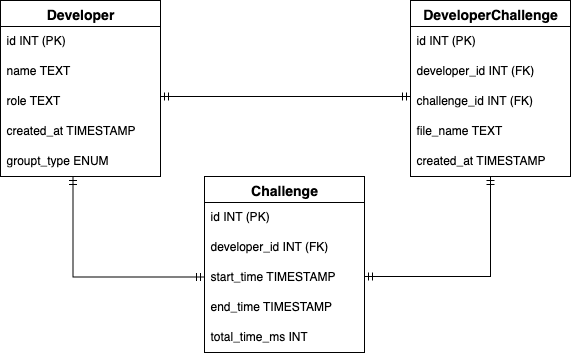
\includegraphics[width=\textwidth]{images/diagrama_er_banco.png}
		\fonte{Elaborado pelo autor}
	\end{minipage}
\end{figure}
\FloatBarrier

\section{TELAS DA APLICAÇÃO}

\renewcommand{\thefigure}{B.\arabic{figure}}
\setcounter{figure}{0}

\begin{figure}[ht]
    \caption{Exemplo 1 do desafio}
    \label{fig:exemplo1}
    \centering
    \footnotesize
    \begin{minipage}{.9\textwidth}
        \centering
        \fbox{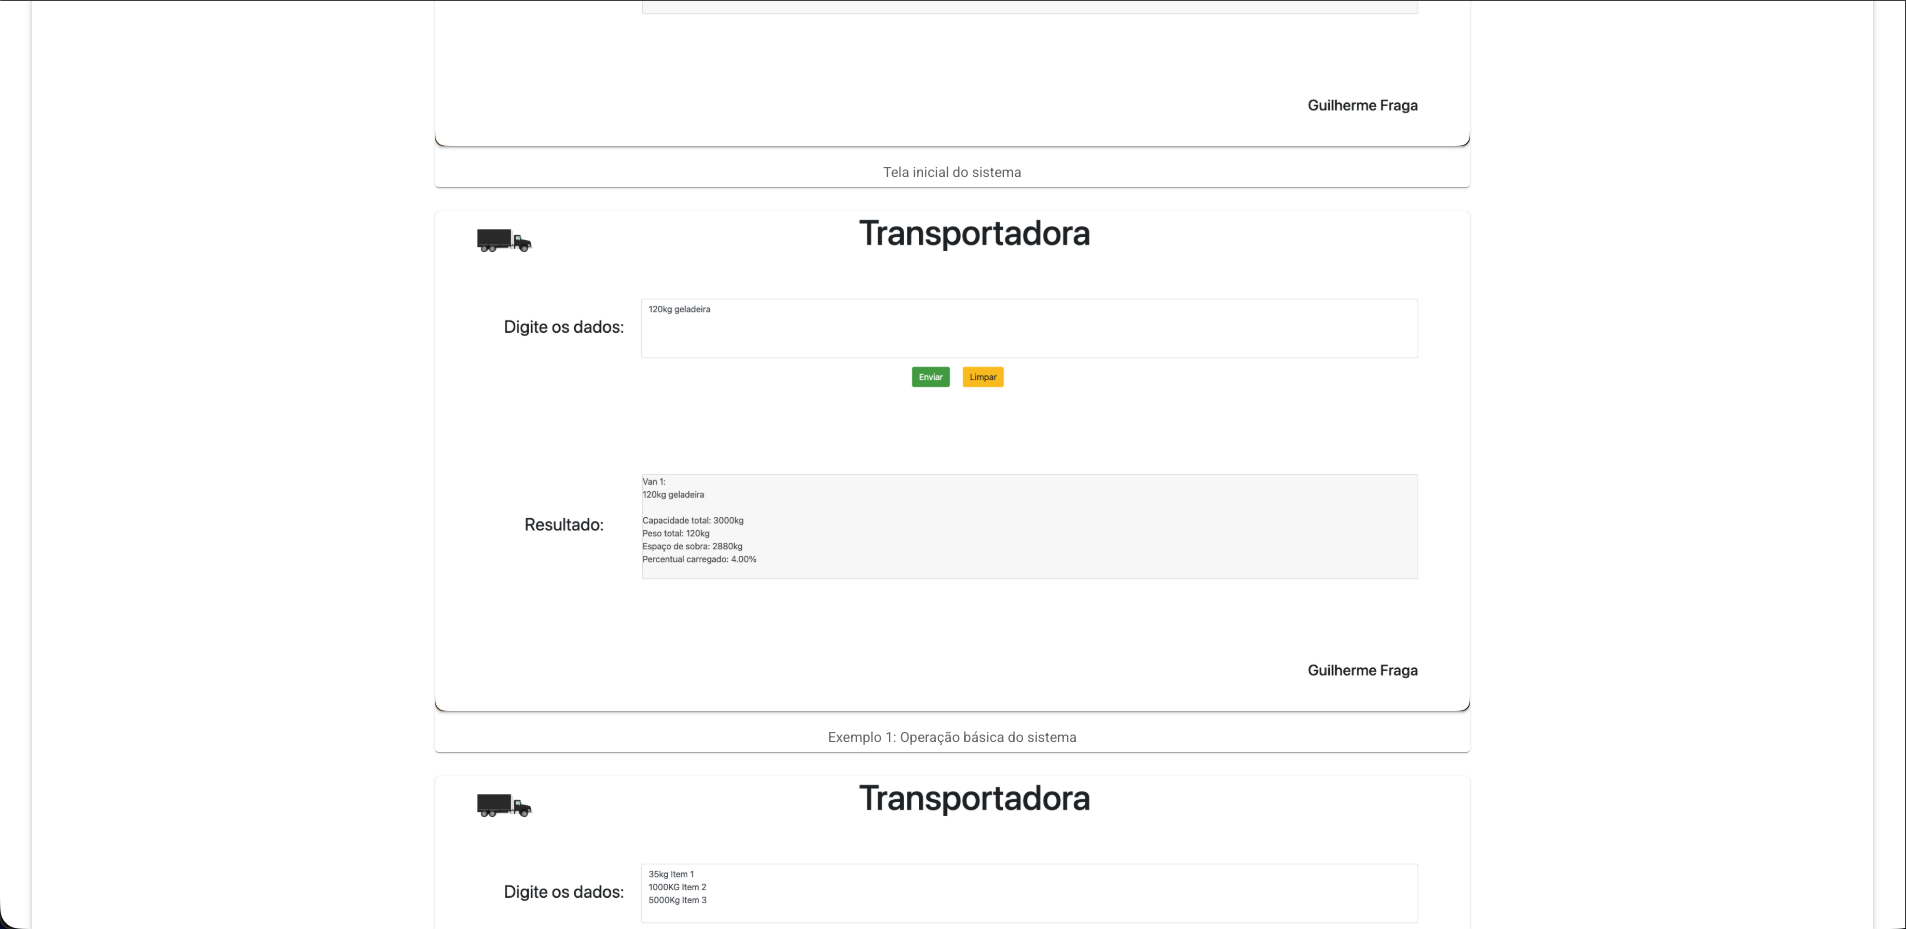
\includegraphics[width=0.95\textwidth]{images/exemplo1.png}}
        \fonte{Elaborado pelo autor}
    \end{minipage}
\end{figure}
\FloatBarrier

\begin{figure}[ht]
    \caption{Exemplo 2 do desafio}
    \label{fig:exemplo2}
    \centering
    \footnotesize
    \begin{minipage}{.9\textwidth}
        \centering
        \fbox{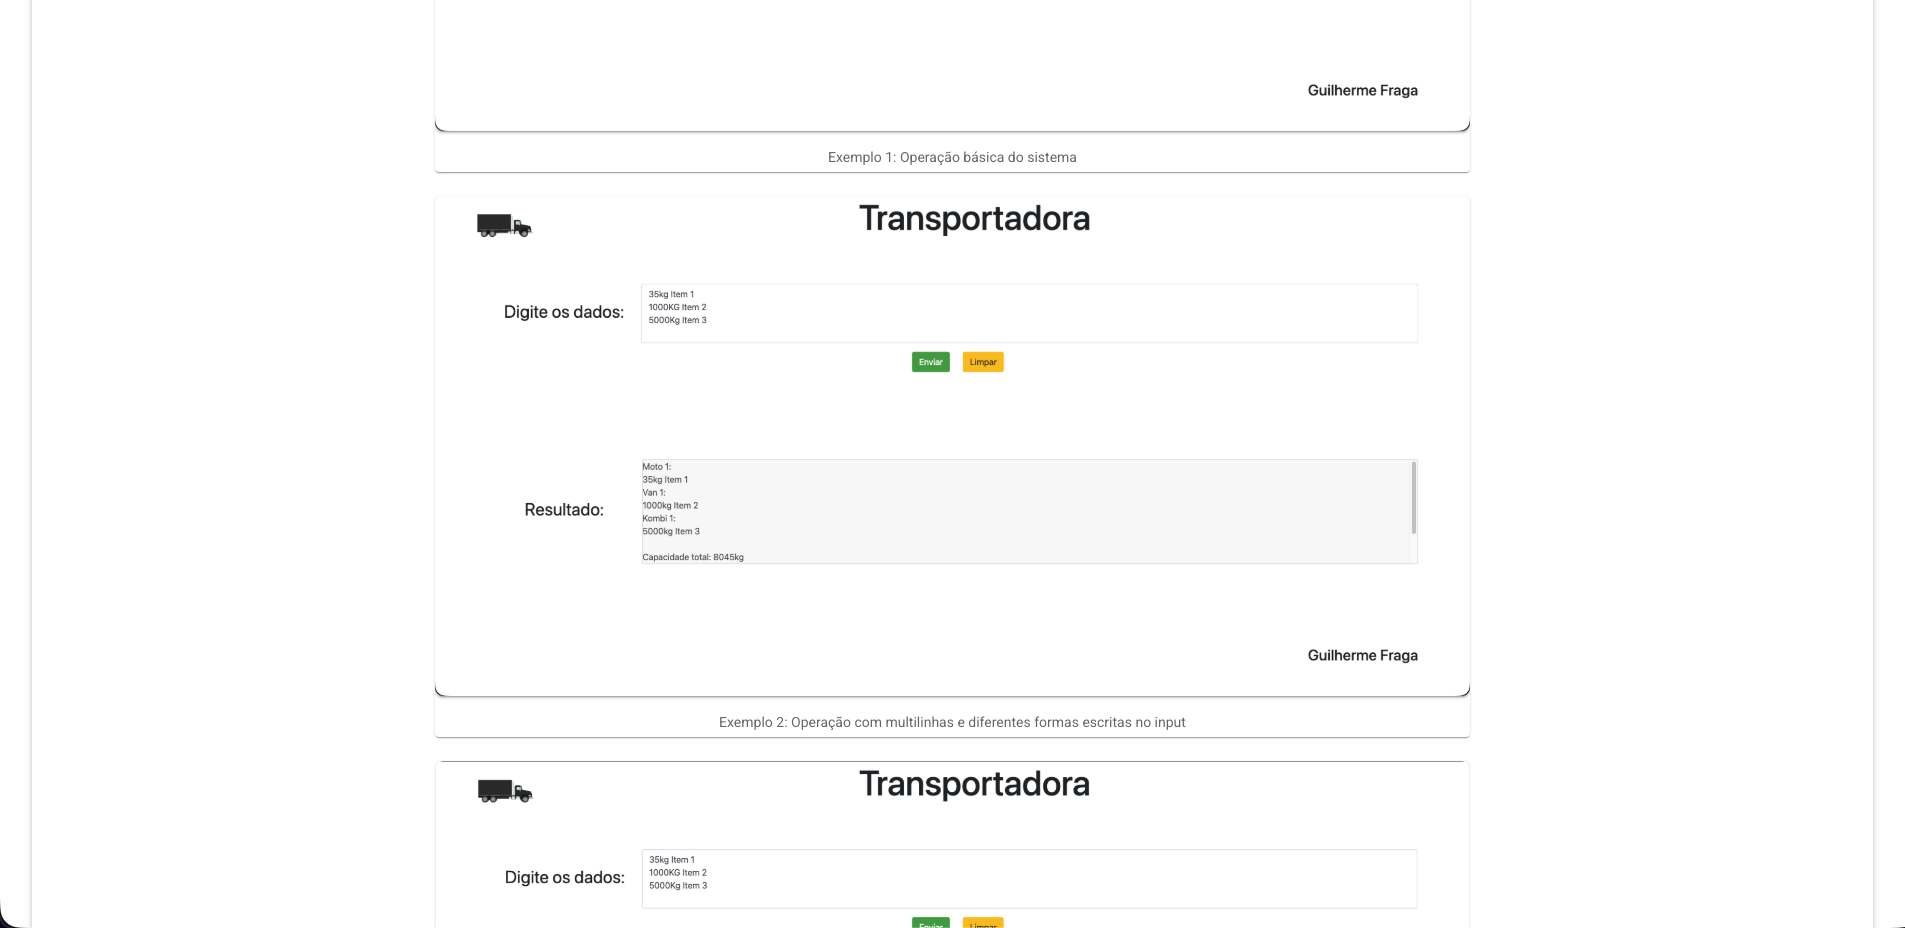
\includegraphics[width=0.95\textwidth]{images/exemplo2.png}}
        \fonte{Elaborado pelo autor}
    \end{minipage}
\end{figure}
\FloatBarrier

\begin{figure}[ht]
    \caption{Exemplo 2.1 do desafio}
    \label{fig:exemplo2_1}
    \centering
    \footnotesize
    \begin{minipage}{.9\textwidth}
        \centering
        \fbox{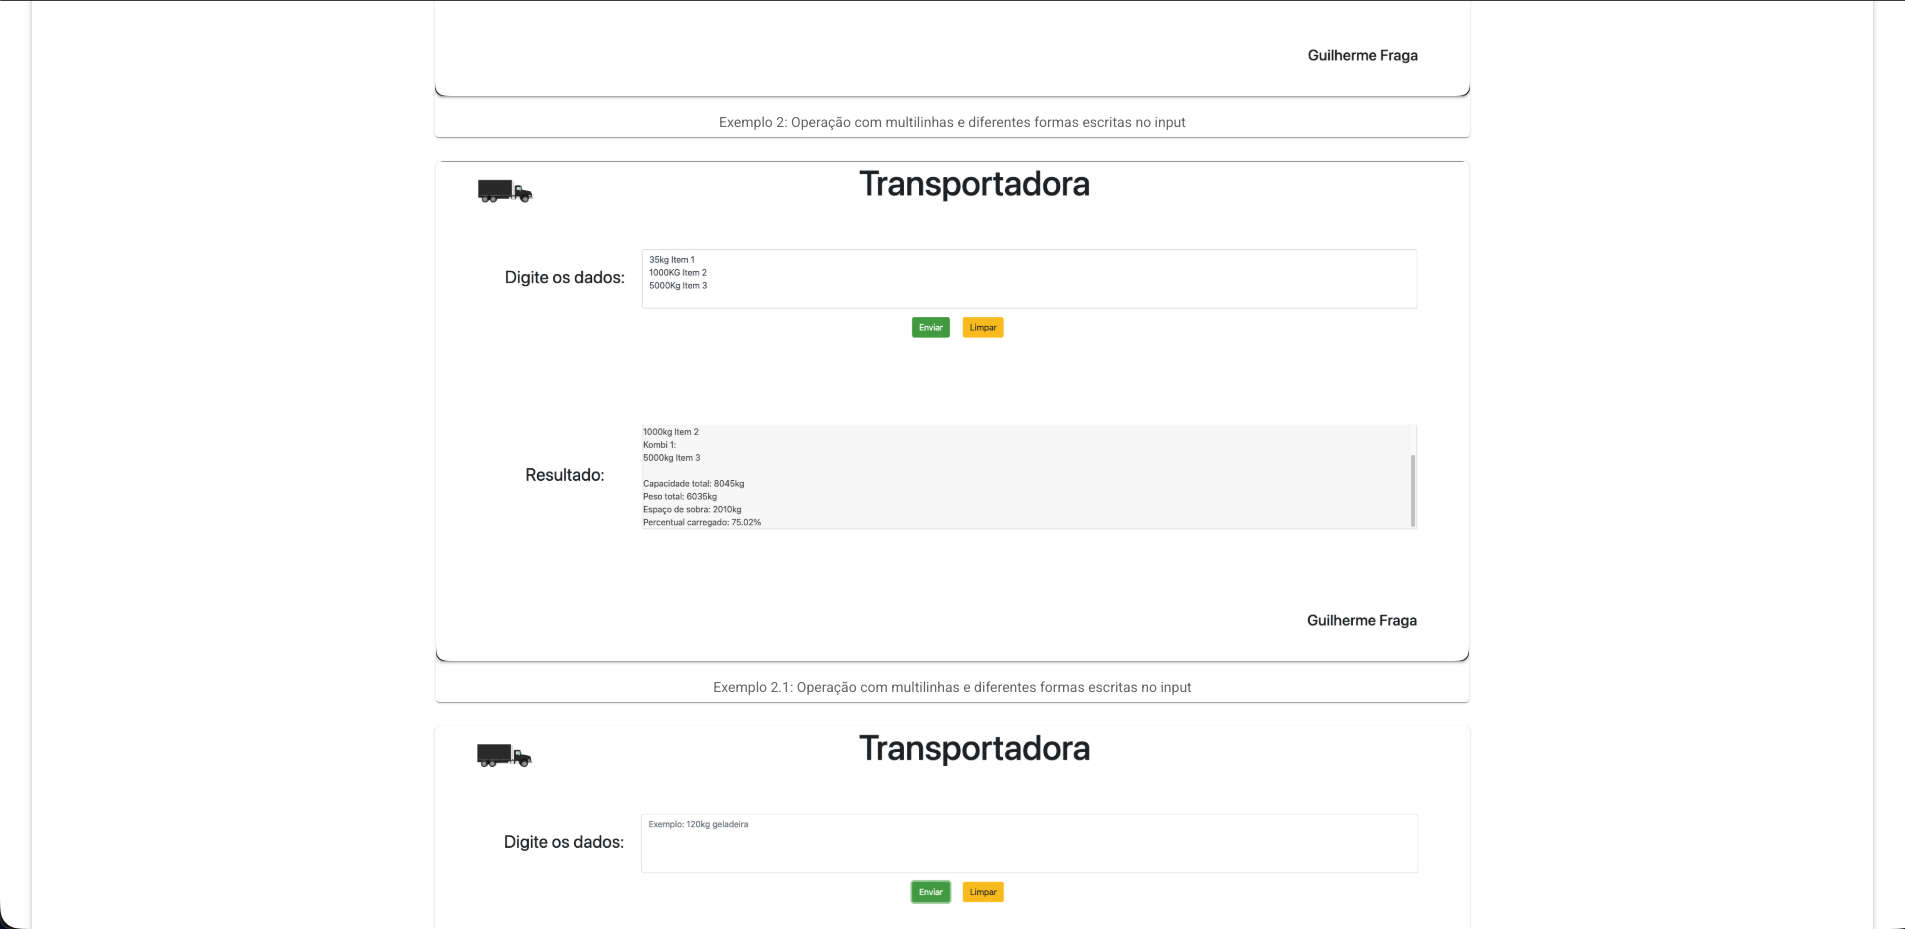
\includegraphics[width=0.95\textwidth]{images/exemplo2.1.png}}
        \fonte{Elaborado pelo autor}
    \end{minipage}
\end{figure}
\FloatBarrier

\begin{figure}[ht]
    \caption{Exemplo 3 do desafio}
    \label{fig:exemplo3}
    \centering
    \footnotesize
    \begin{minipage}{.9\textwidth}
        \centering
        \fbox{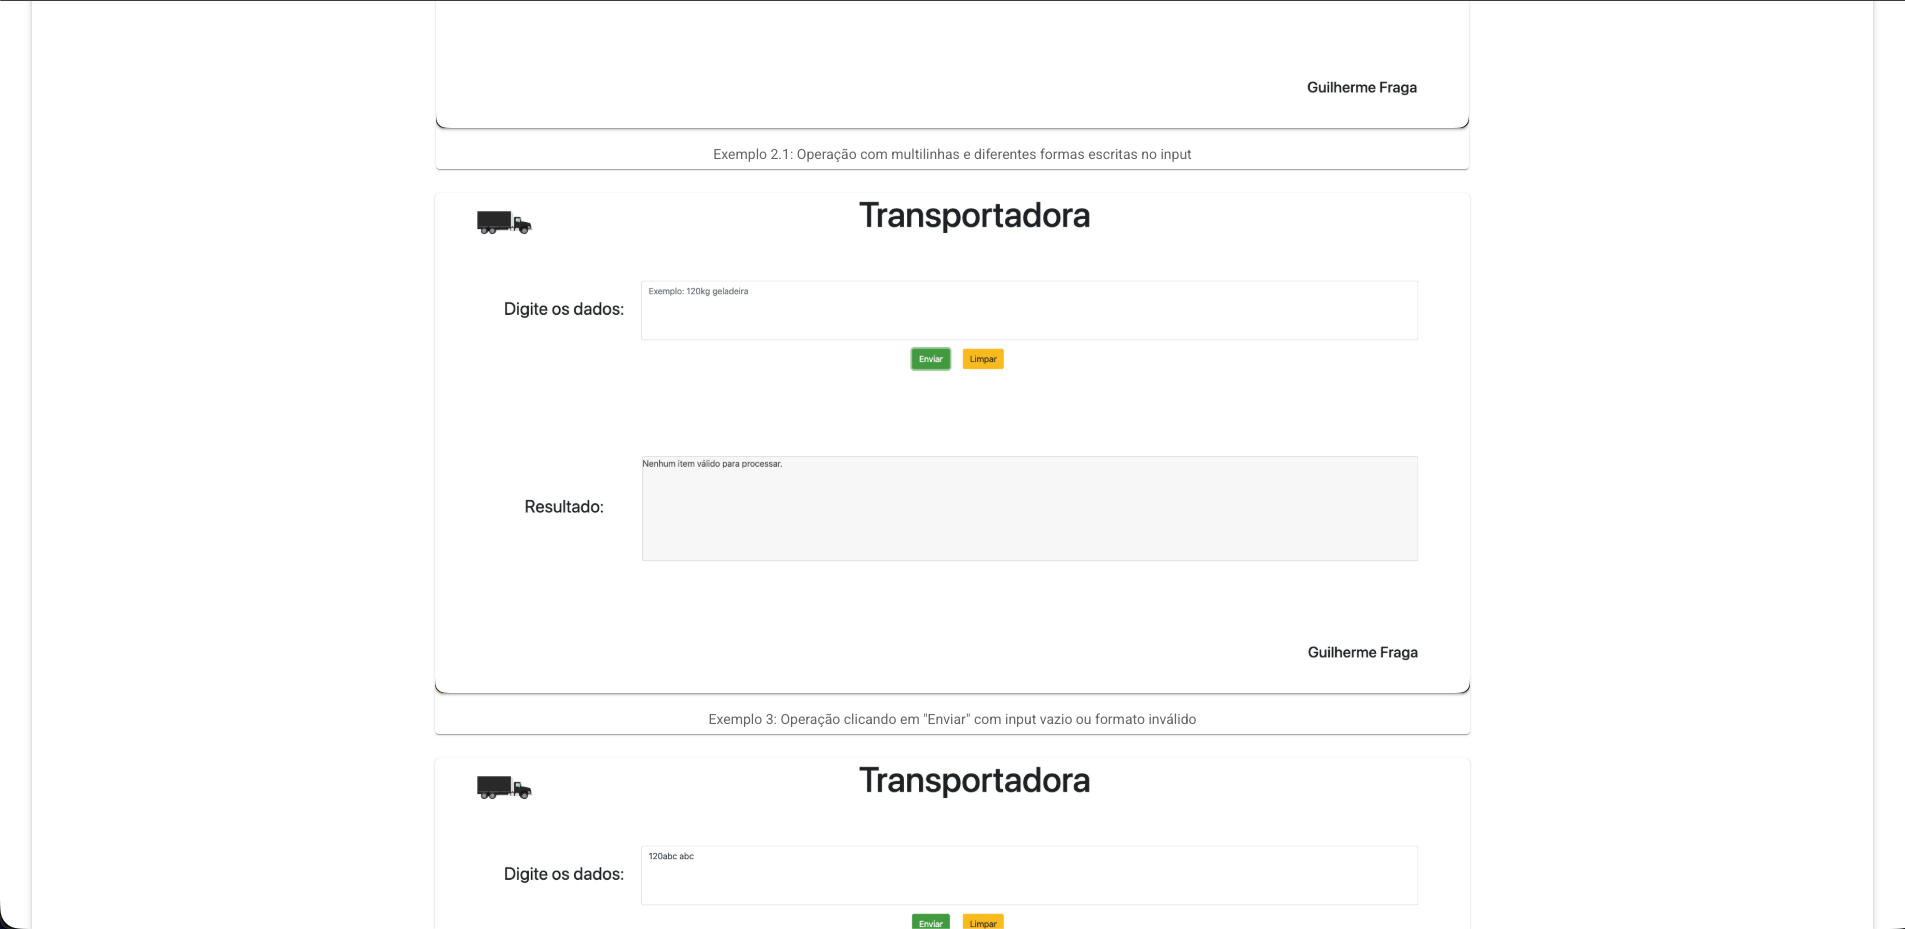
\includegraphics[width=0.95\textwidth]{images/exemplo3.png}}
        \fonte{Elaborado pelo autor}
    \end{minipage}
\end{figure}
\FloatBarrier

\begin{figure}[ht]
    \caption{Exemplo 3.1 do desafio}
    \label{fig:exemplo3_1}
    \centering
    \footnotesize
    \begin{minipage}{.9\textwidth}
        \centering
        \fbox{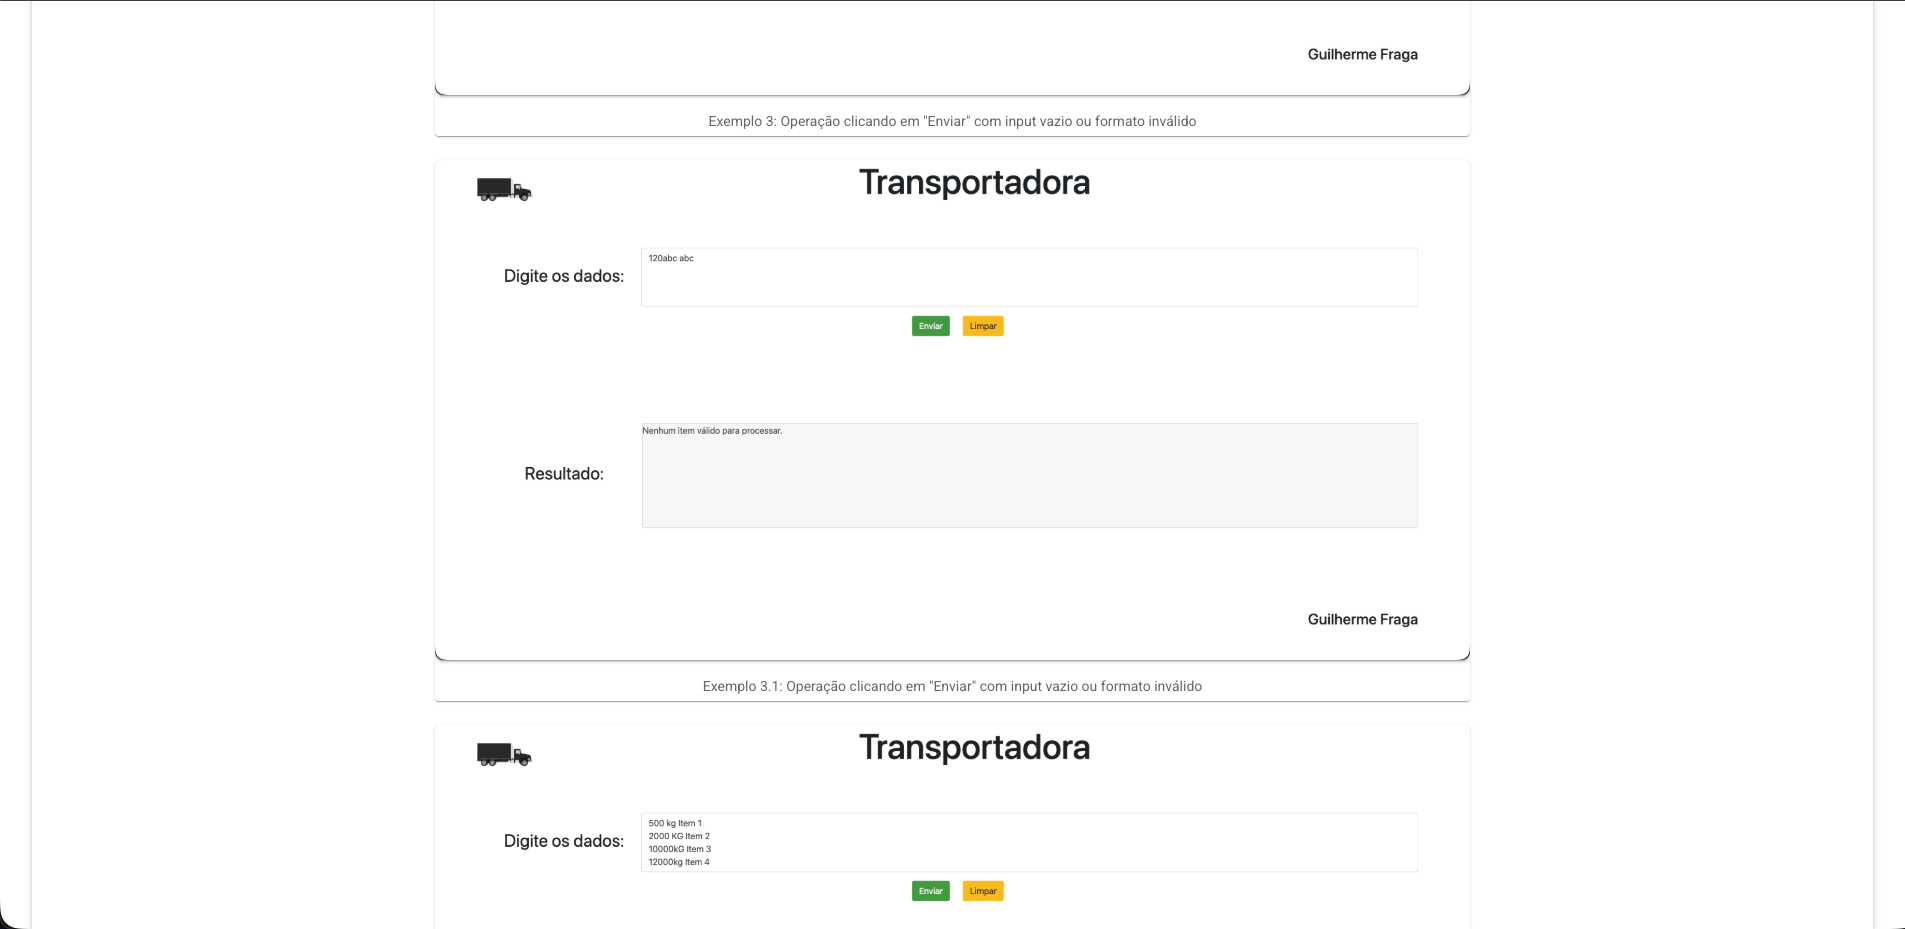
\includegraphics[width=0.95\textwidth]{images/exemplo3.1.png}}
        \fonte{Elaborado pelo autor}
    \end{minipage}
\end{figure}
\FloatBarrier

\begin{figure}[ht]
    \caption{Exemplo 4 do desafio}
    \label{fig:exemplo4}
    \centering
    \footnotesize
    \begin{minipage}{.9\textwidth}
        \centering
        \fbox{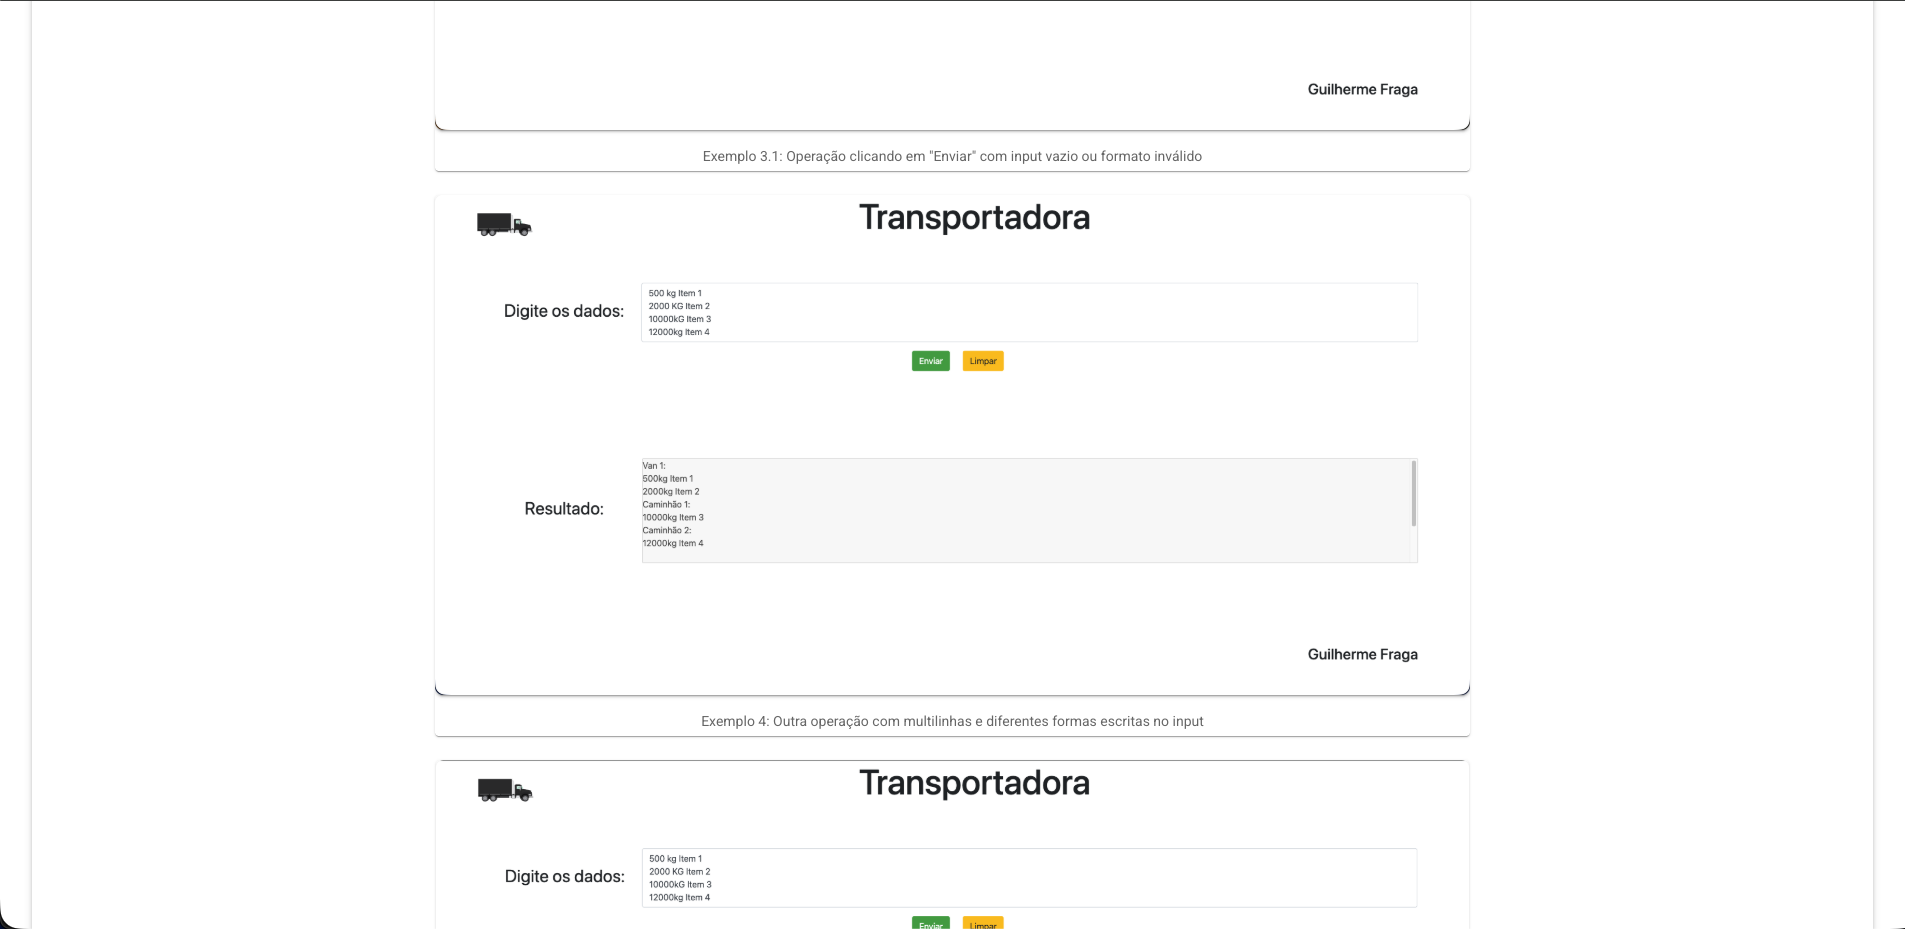
\includegraphics[width=0.95\textwidth]{images/exemplo4.png}}
        \fonte{Elaborado pelo autor}
    \end{minipage}
\end{figure}
\FloatBarrier

\begin{figure}[ht]
    \caption{Exemplo 4.1 do desafio}
    \label{fig:exemplo4_1}
    \centering
    \footnotesize
    \begin{minipage}{.9\textwidth}
        \centering
        \fbox{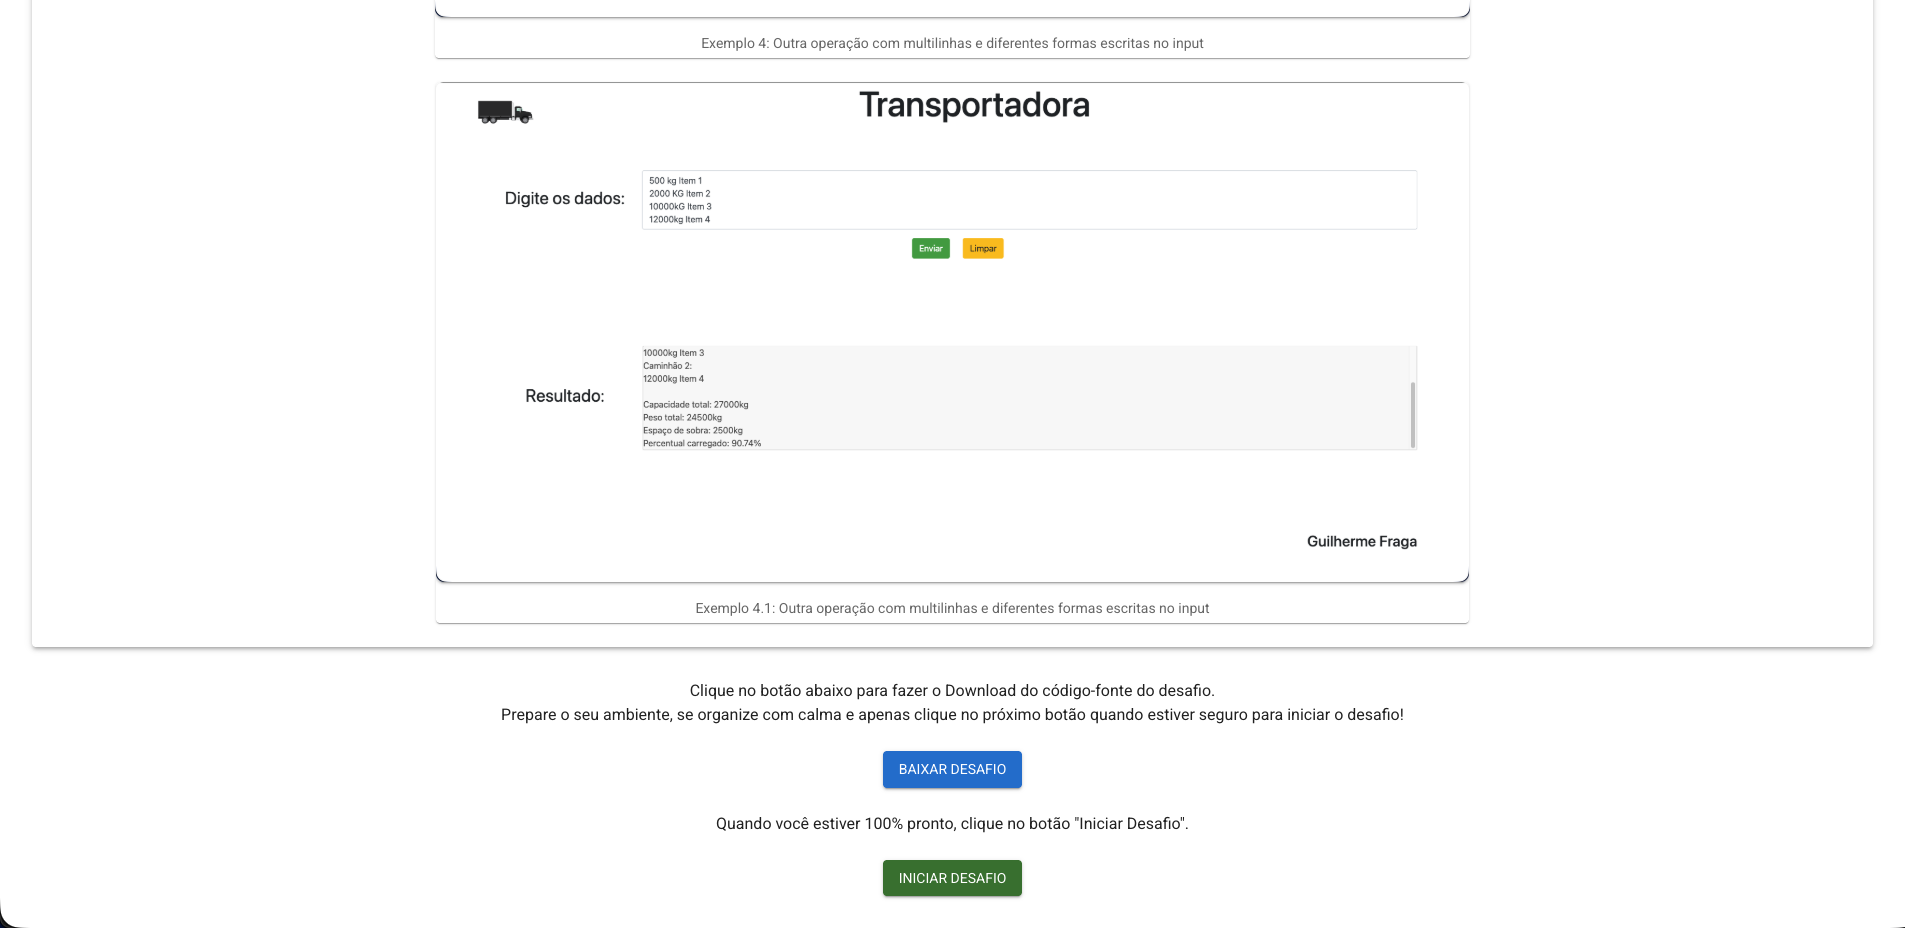
\includegraphics[width=0.95\textwidth]{images/exemplo4.1.png}}
        \fonte{Elaborado pelo autor}
    \end{minipage}
\end{figure}
\FloatBarrier

\begin{figure}[ht]
    \caption{Editar arquivo e finalizar desafio}
    \label{fig:arquivo_salvo_finalizar_desafio}
    \centering
    \footnotesize
    \begin{minipage}{.9\textwidth}
        \centering
        \fbox{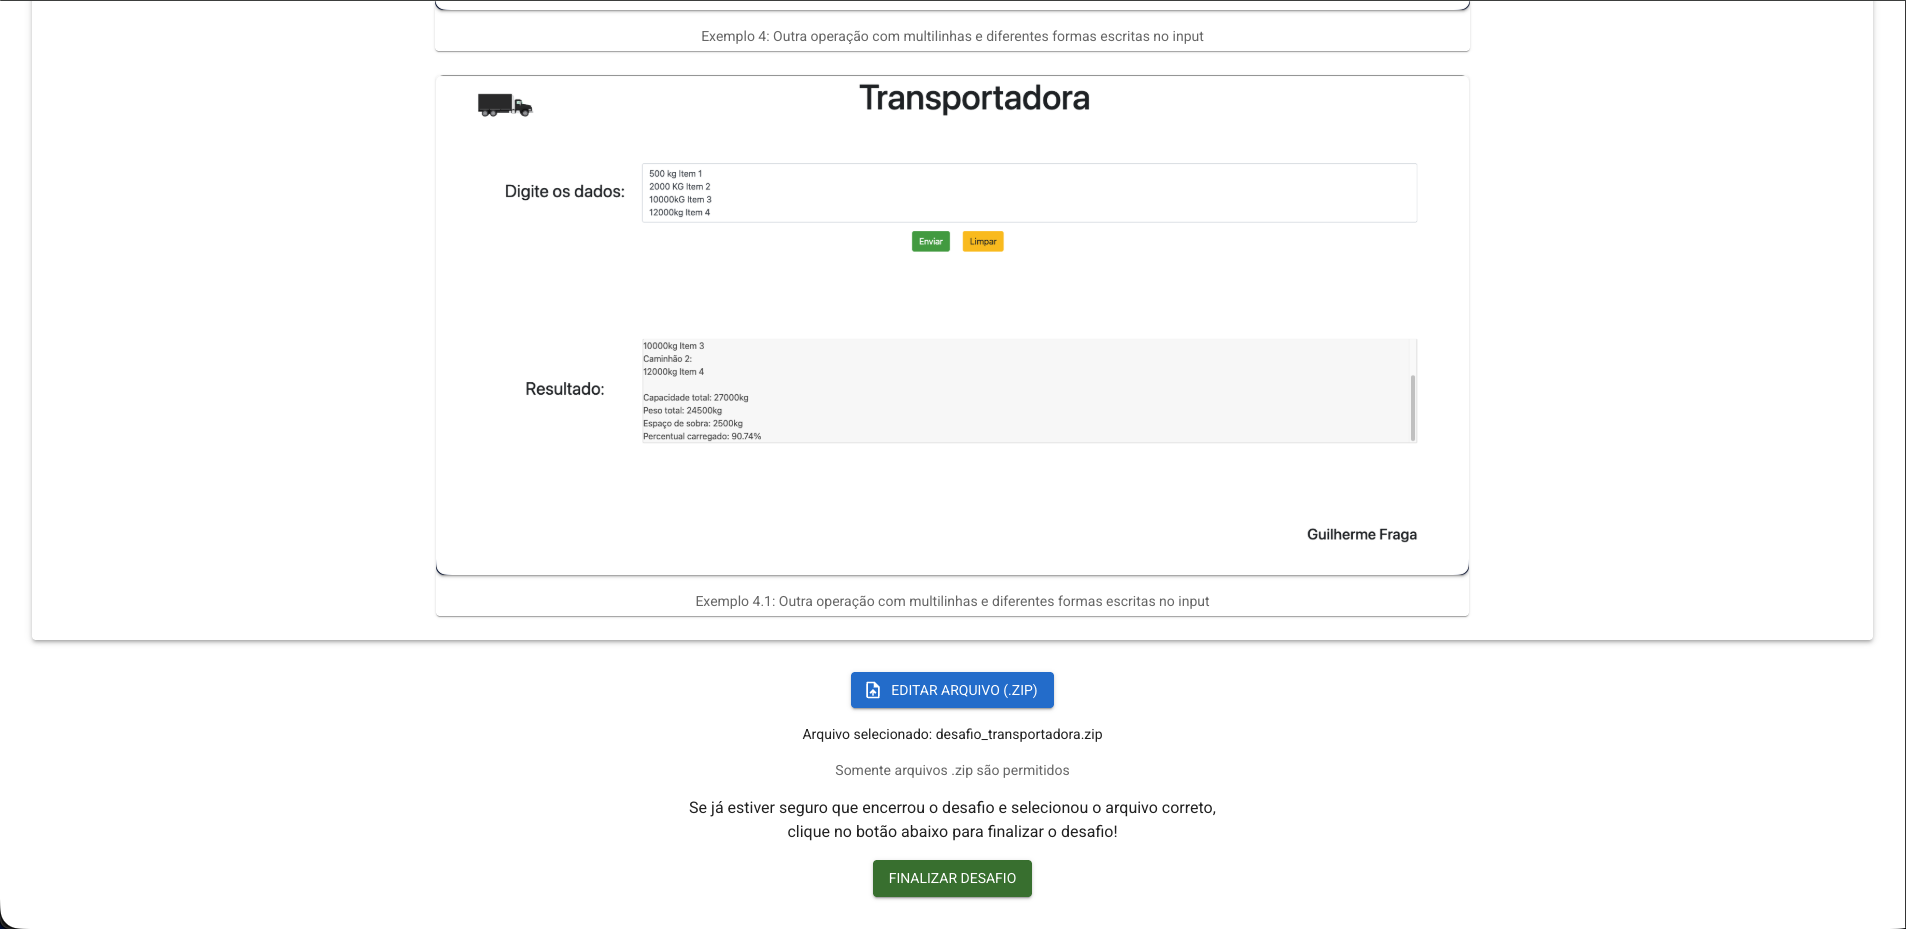
\includegraphics[width=0.95\textwidth]{images/arquivo_salvo_finalizar_desafio.png}}
        \fonte{Elaborado pelo autor}
    \end{minipage}
\end{figure}
\FloatBarrier

\section{INSTRUÇÕES ENVIADAS AOS PARTICIPANTES VIA \textit{WHATSAPP}}

\renewcommand{\thefigure}{C.\arabic{figure}}
\setcounter{figure}{0}

\begin{figure}[ht]
    \caption{Instruções enviadas via \textit{WhatsApp} para o grupo sem IA}
    \label{fig:instrucoes_sem_ia}
    \centering
    \footnotesize
    \begin{minipage}{.9\textwidth}
        \centering
        \fbox{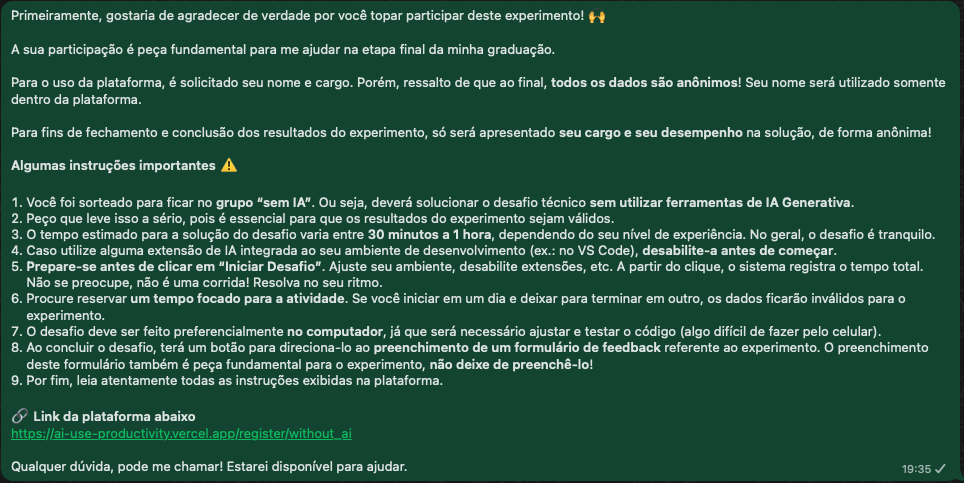
\includegraphics[width=0.95\textwidth]{images/instrucoes_sem_ia.png}}
        \fonte{Elaborado pelo autor}
    \end{minipage}
\end{figure}
\FloatBarrier

\begin{figure}[ht]
    \caption{Instruções enviadas via \textit{WhatsApp} para o grupo com IA}
    \label{fig:instrucoes_com_ia}
    \centering
    \footnotesize
    \begin{minipage}{.9\textwidth}
        \centering
        \fbox{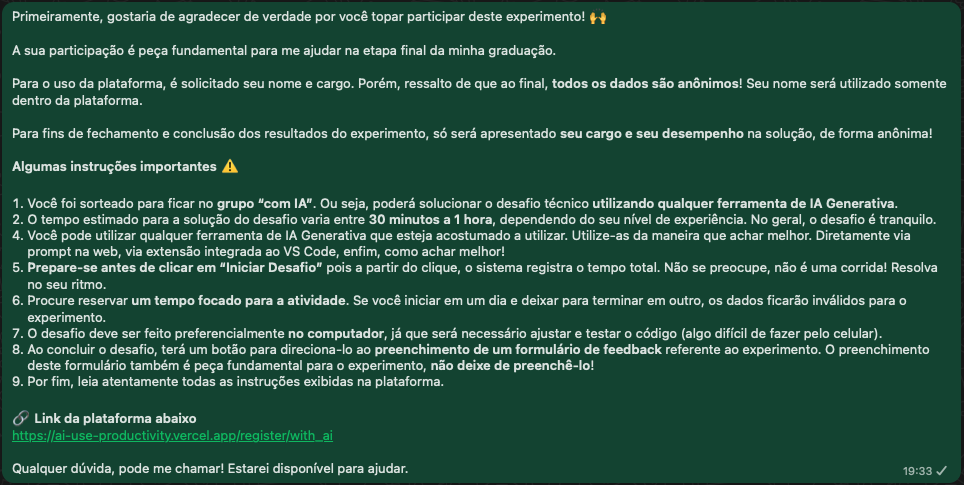
\includegraphics[width=0.95\textwidth]{images/instrucoes_com_ia.png}}
        \fonte{Elaborado pelo autor}
    \end{minipage}
\end{figure}
\FloatBarrier

\section{CENÁRIOS DE TESTES}

O desenvolvedor deveria replicar os \textit{inputs} exibidos nas imagens de exemplo, que representavam os resultados esperados no \textit{output}. Estes foram os \textit{inputs} aplicados ao testes na interface \textit{HTML} e comparado com o código-fonte base funcional para verificar se os resultados estavam coerentes.

\textbf{Cenário 1}

\begin{itemize}[leftmargin=1cm, itemsep=0.1em, topsep=0.1em]
    \item \textit{input}
    \begin{itemize}[leftmargin=1.2cm, itemsep=0.1em, topsep=0.1em]
        120kg geladeira
    \end{itemize}
    \item \textit{output}
    \begin{itemize}[leftmargin=1.2cm, itemsep=0.1em, topsep=0.1em]
        Van 1:\\
        120kg geladeira\\
        
        \\Capacidade total: 3000kg\\
        Peso total: 120kg\\
        Espaço de sobra: 2880kg\\
        Percentual carregado: 4.00\%
    \end{itemize}
\end{itemize}

\textbf{Cenário 2}

\begin{itemize}[leftmargin=1cm, itemsep=0.1em, topsep=0.1em]
    \item \textit{input}
    \begin{itemize}[leftmargin=1.2cm, itemsep=0.1em, topsep=0.1em]
        35kg Item 1\\
        1000KG Item 2\\
        5000Kg Item 3
    \end{itemize}
    \item \textit{output}
    \begin{itemize}[leftmargin=1.2cm, itemsep=0.1em, topsep=0.1em]
        Moto 1:\\
        35kg Item 1\\
        Van 1:\\ 
        1000kg Item 2\\
        Kombi 1:\\
        5000kg Item 3\\

        \\Capacidade total: 8045kg\\
        Peso total: 6035kg\\
        Espaço de sobra: 2010kg\\
        Percentual carregado: 75.02\%
    \end{itemize}
\end{itemize}

\textbf{Cenário 3}

\begin{itemize}[leftmargin=1cm, itemsep=0.1em, topsep=0.1em]
    \item \textit{input}
    \begin{itemize}[leftmargin=1.2cm, itemsep=0.1em, topsep=0.1em]
        vazio
    \end{itemize}
    \item \textit{output}
    \begin{itemize}[leftmargin=1.2cm, itemsep=0.1em, topsep=0.1em]
        Nenhum item válido para processar.
    \end{itemize}
\end{itemize}

\textbf{Cenário 4}

\begin{itemize}[leftmargin=1cm, itemsep=0.1em, topsep=0.1em]
    \item \textit{input}
    \begin{itemize}[leftmargin=1.2cm, itemsep=0.1em, topsep=0.1em]
        120abc abc
    \end{itemize}
    \item \textit{output}
    \begin{itemize}[leftmargin=1.2cm, itemsep=0.1em, topsep=0.1em]
        Nenhum item válido para processar.
    \end{itemize}
\end{itemize}

\textbf{Cenário 5}

\begin{itemize}[leftmargin=1cm, itemsep=0.1em, topsep=0.1em]
    \item \textit{input}
    \begin{itemize}[leftmargin=1.2cm, itemsep=0.1em, topsep=0.1em]
        500 kg Item 1\\
        2000 KG Item 2\\
        10000kG Item 3\\
        12000kg Item 4
    \end{itemize}
    \item \textit{output}
    \begin{itemize}[leftmargin=1.2cm, itemsep=0.1em, topsep=0.1em]
        Van 1:\\
        500kg Item 1\\
        2000kg Item 2\\
        Caminhão 1:\\
        10000kg Item 3\\
        Caminhão 2:\\
        12000kg Item 4\\

        \\Capacidade total: 27000kg\\
        Peso total: 24500kg\\
        Espaço de sobra: 2500kg\\
        Percentual carregado: 90.74\%
    \end{itemize}
\end{itemize}

\section{QUESTIONÁRIOS DE AVALIAÇÃO DO MODELO}

\renewcommand{\thefigure}{E.\arabic{figure}}
\setcounter{figure}{0}

\begin{figure}[ht]
    \caption{Questão 1 e 2 do formulário final para todos os participantes}
    \label{fig:questao1_2_geral}
    \centering
    \footnotesize
    \begin{minipage}{.9\textwidth}
        \centering
        \fbox{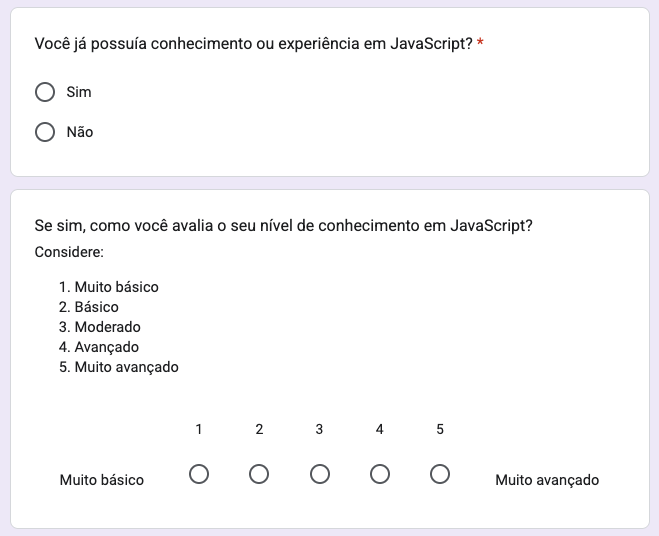
\includegraphics[width=0.95\textwidth]{images/questao1_2_geral.png}}
        \fonte{Elaborado pelo autor}
    \end{minipage}
\end{figure}
\FloatBarrier

\begin{figure}[ht]
    \caption{Questão 3 e 4 do formulário final para todos os participantes}
    \label{fig:questao3_4_geral}
    \centering
    \footnotesize
    \begin{minipage}{.9\textwidth}
        \centering
        \fbox{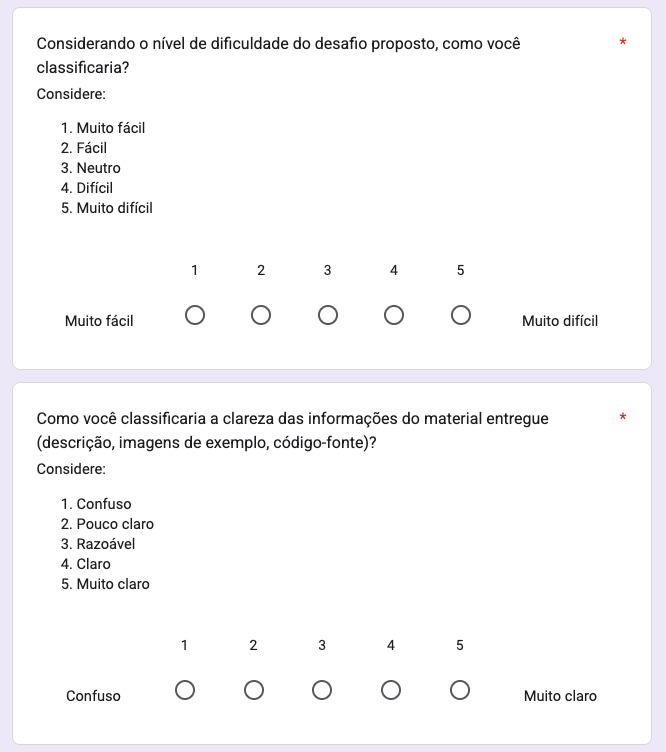
\includegraphics[width=0.95\textwidth]{images/questao3_4_geral.png}}
        \fonte{Elaborado pelo autor}
    \end{minipage}
\end{figure}
\FloatBarrier

\begin{figure}[ht]
    \caption{Questão 5 e 6 do formulário final para todos os participantes}
    \label{fig:questao5_6_geral}
    \centering
    \footnotesize
    \begin{minipage}{.9\textwidth}
        \centering
        \fbox{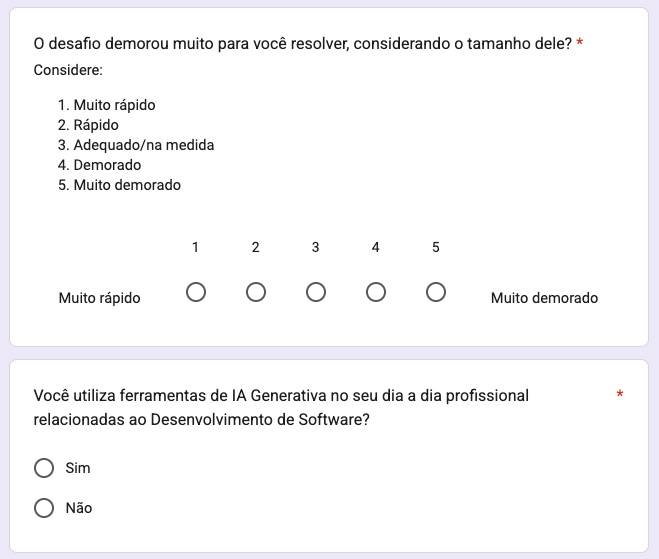
\includegraphics[width=0.95\textwidth]{images/questao5_6_geral.png}}
        \fonte{Elaborado pelo autor}
    \end{minipage}
\end{figure}
\FloatBarrier

\begin{figure}[ht]
    \caption{Questão 7 do formulário final para todos os participantes}
    \label{fig:questao7_geral}
    \centering
    \footnotesize
    \begin{minipage}{.9\textwidth}
        \centering
        \fbox{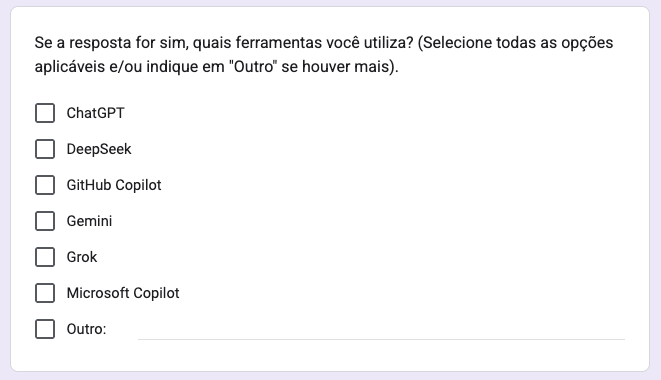
\includegraphics[width=0.95\textwidth]{images/questao7_geral.png}}
        \fonte{Elaborado pelo autor}
    \end{minipage}
\end{figure}
\FloatBarrier

\begin{figure}[ht]
    \caption{Questão 8, 9 e 10 do formulário final para todos os membros do grupo sem IA}
    \label{fig:questao8_9_10_sem_ia}
    \centering
    \footnotesize
    \begin{minipage}{.9\textwidth}
        \centering
        \fbox{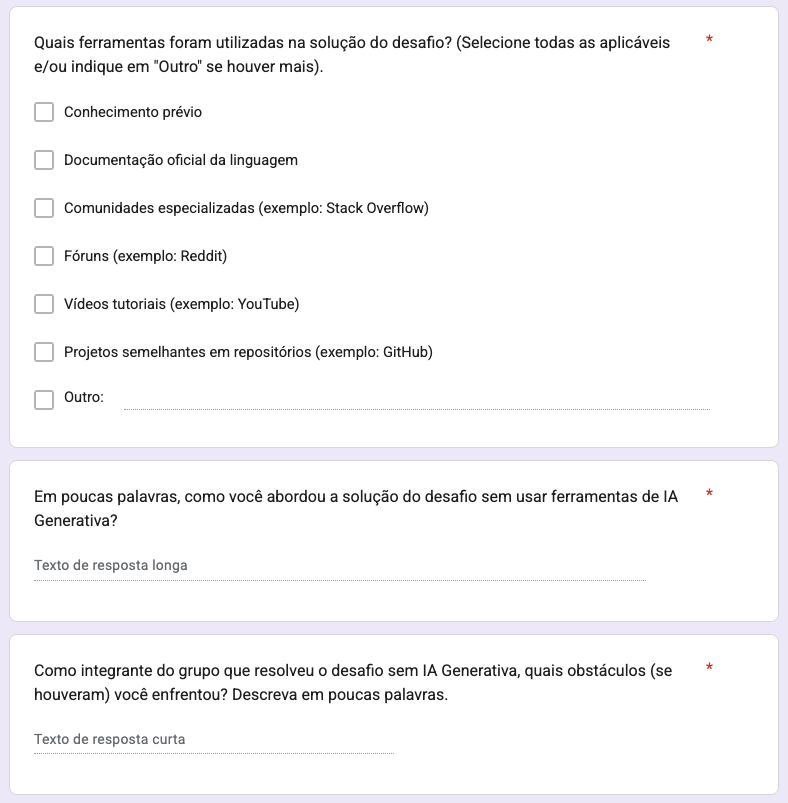
\includegraphics[width=0.95\textwidth]{images/questao8_9_10_sem_ia.png}}
        \fonte{Elaborado pelo autor}
    \end{minipage}
\end{figure}
\FloatBarrier

\begin{figure}[ht]
    \caption{Questão 8, 9 e 10 do formulário final para todos os membros do grupo com IA}
    \label{fig:questao8_9_10_com_ia}
    \centering
    \footnotesize
    \begin{minipage}{.9\textwidth}
        \centering
        \fbox{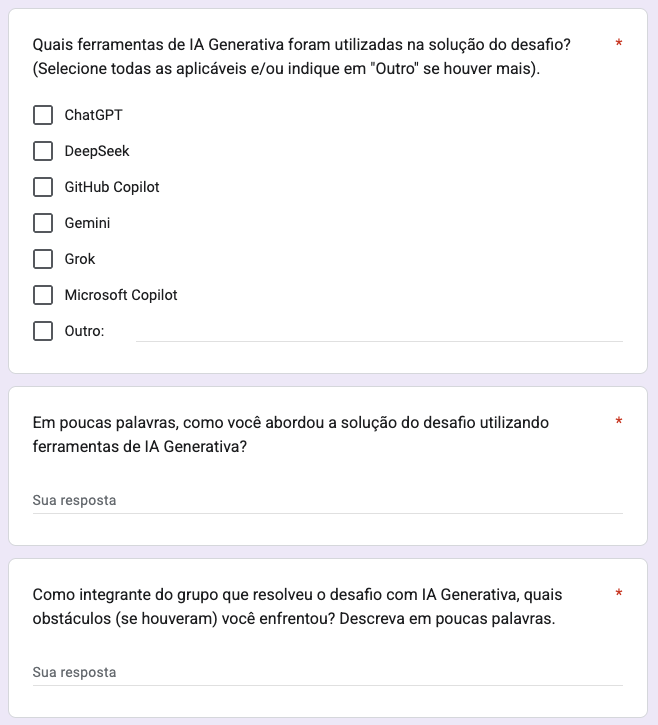
\includegraphics[width=0.95\textwidth]{images/questao8_9_10_com_ia.png}}
        \fonte{Elaborado pelo autor}
    \end{minipage}
\end{figure}
\FloatBarrier

\begin{figure}[ht]
    \caption{Questão 11 do formulário final para todos os participantes}
    \label{fig:questao11_geral}
    \centering
    \footnotesize
    \begin{minipage}{.9\textwidth}
        \centering
        \fbox{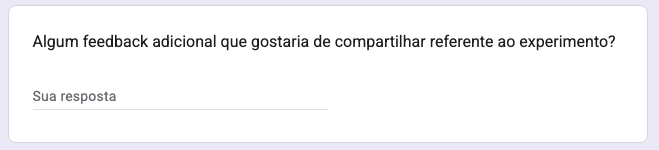
\includegraphics[width=0.95\textwidth]{images/questao11_geral.png}}
        \fonte{Elaborado pelo autor}
    \end{minipage}
\end{figure}
\FloatBarrier

\section{RESPOSTAS DO FORMULÁRIO}

\renewcommand{\thefigure}{F.\arabic{figure}}
\setcounter{figure}{0}

\renewcommand{\thetable}{F.\arabic{table}}
\setcounter{table}{0}

Os gráficos e quadros abaixo representam as respostas completas do questionário, dos grupos sem IA e com IA, respectivamente. Os Gráficos \ref{graf:resposta1_sem_ia} e \ref{graf:resposta1_com_ia} referem-se à questão 1. Os Gráficos \ref{graf:resposta2_sem_ia} e \ref{graf:resposta2_com_ia} são as respostas da questão 2. Os Gráficos \ref{graf:resposta3_sem_ia} e \ref{graf:resposta3_com_ia} referem-se à questão 3. Os Gráficos \ref{graf:resposta4_sem_ia} e \ref{graf:resposta4_com_ia} são da questão 4. Os Gráficos \ref{graf:resposta5_sem_ia} e \ref{graf:resposta5_com_ia} são referentes à questão 5. Os Gráficos \ref{graf:resposta6_sem_ia} e \ref{graf:resposta6_com_ia} tratam-se da questão 6. Os Gráfico \ref{graf:resposta7_sem_ia} e \ref{graf:resposta7_com_ia} referem-se à questão 7. Os Gráficos \ref{graf:resposta8_sem_ia} e \ref{graf:resposta8_com_ia} são as repostas da questão 8.

As Tabelas \ref{tab:questao9_sem_ia} e \ref{tab:questao9_com_ia} referem-se à questão 9. As Tabelas \ref{tab:questao10_sem_ia} e \ref{tab:questao10_com_ia} são as respostas da questão 10. Por fim, as tabelas \ref{tab:questao11_sem_ia} e \ref{tab:questao11_com_ia} tratam-se da questão 11.

\begin{figure}[ht]
    \caption{Respotas da questão 1 de todos do grupo sem IA}
    \label{graf:resposta1_sem_ia}
    \centering
    \footnotesize
    \begin{minipage}{.9\textwidth}
        \centering
        \fbox{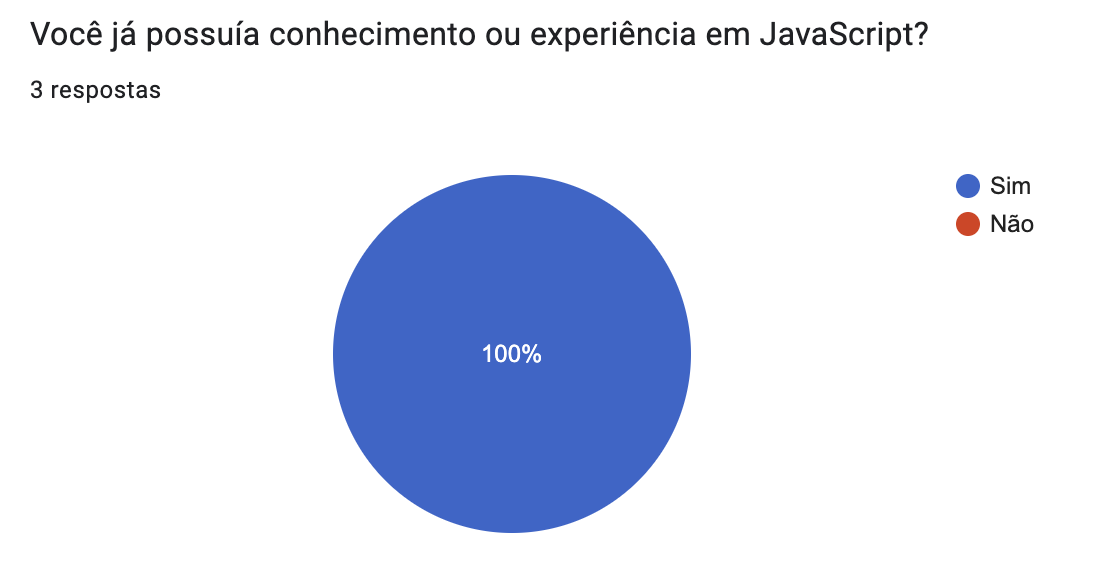
\includegraphics[width=0.95\textwidth]{images/resposta1_sem_com_ia.png}}
        \fonte{Elaborado pelo autor}
    \end{minipage}
\end{figure}
\FloatBarrier

\begin{figure}[ht]
    \caption{Respotas da questão 1 de todos do grupo com IA}
    \label{graf:resposta1_com_ia}
    \centering
    \footnotesize
    \begin{minipage}{.9\textwidth}
        \centering
        \fbox{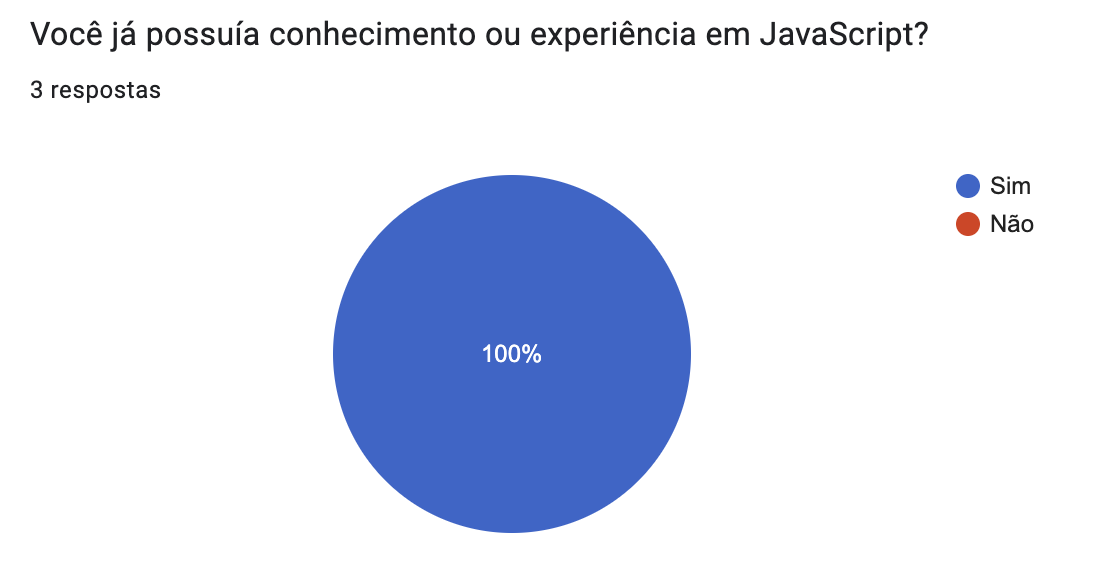
\includegraphics[width=0.95\textwidth]{images/resposta1_sem_com_ia.png}}
        \fonte{Elaborado pelo autor}
    \end{minipage}
\end{figure}
\FloatBarrier

\begin{figure}[ht]
    \caption{Respotas da questão 2 de todos do grupo sem IA}
    \label{graf:resposta2_sem_ia}
    \centering
    \footnotesize
    \begin{minipage}{.9\textwidth}
        \centering
        \fbox{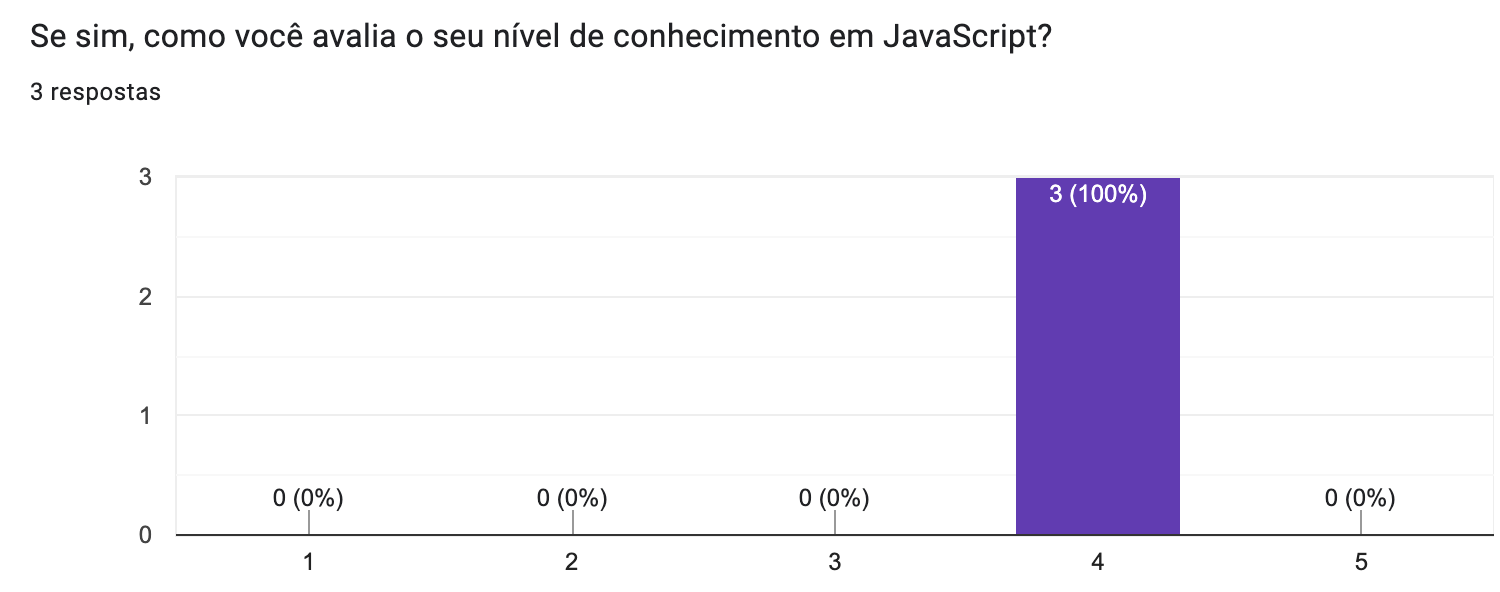
\includegraphics[width=0.95\textwidth]{images/resposta2_sem_ia.png}}
        \fonte{Elaborado pelo autor}
    \end{minipage}
\end{figure}
\FloatBarrier

\begin{figure}[ht]
    \caption{Respotas da questão 2 de todos do grupo com IA}
    \label{graf:resposta2_com_ia}
    \centering
    \footnotesize
    \begin{minipage}{.9\textwidth}
        \centering
        \fbox{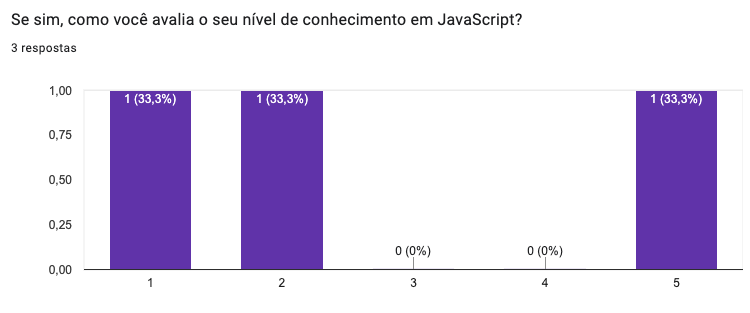
\includegraphics[width=0.95\textwidth]{images/resposta2_com_ia.png}}
        \fonte{Elaborado pelo autor}
    \end{minipage}
\end{figure}
\FloatBarrier

\begin{figure}[ht]
    \caption{Respotas da questão 3 de todos do grupo sem IA}
    \label{graf:resposta3_sem_ia}
    \centering
    \footnotesize
    \begin{minipage}{.9\textwidth}
        \centering
        \fbox{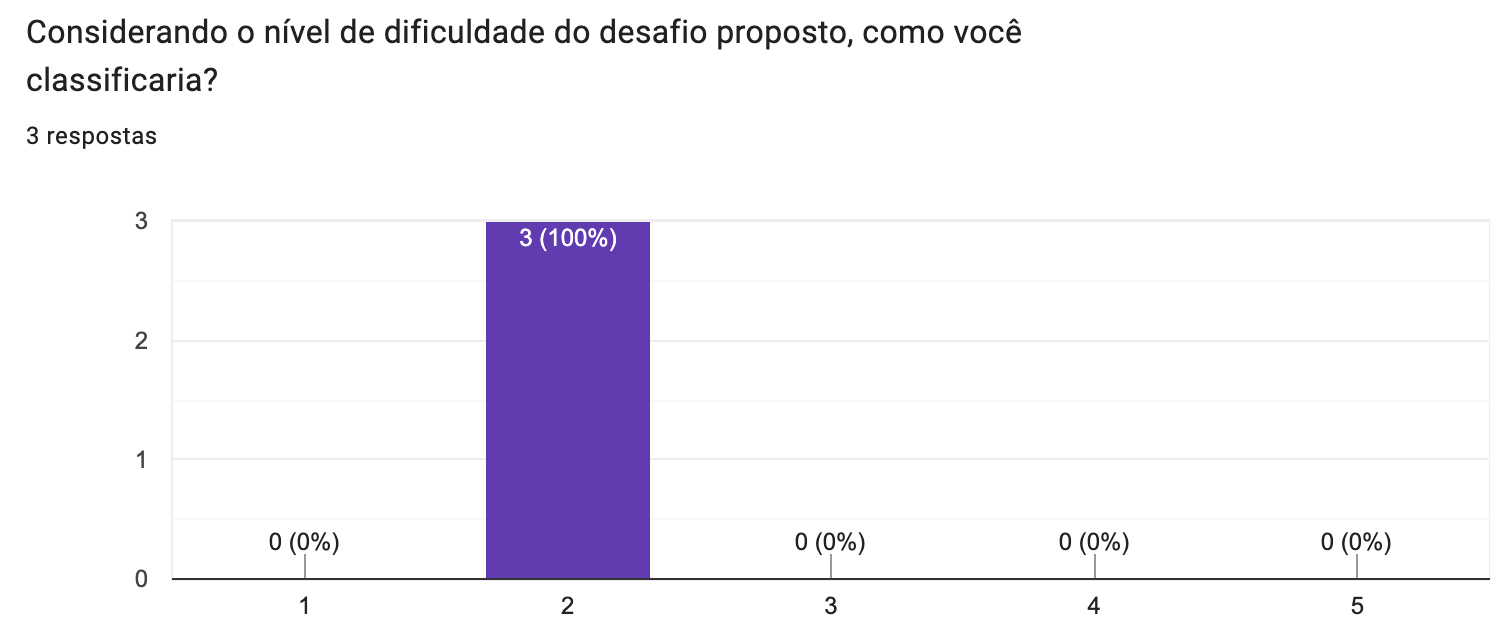
\includegraphics[width=0.95\textwidth]{images/resposta3_sem_ia.png}}
        \fonte{Elaborado pelo autor}
    \end{minipage}
\end{figure}
\FloatBarrier

\begin{figure}[ht]
    \caption{Respotas da questão 3 de todos do grupo com IA}
    \label{graf:resposta3_com_ia}
    \centering
    \footnotesize
    \begin{minipage}{.9\textwidth}
        \centering
        \fbox{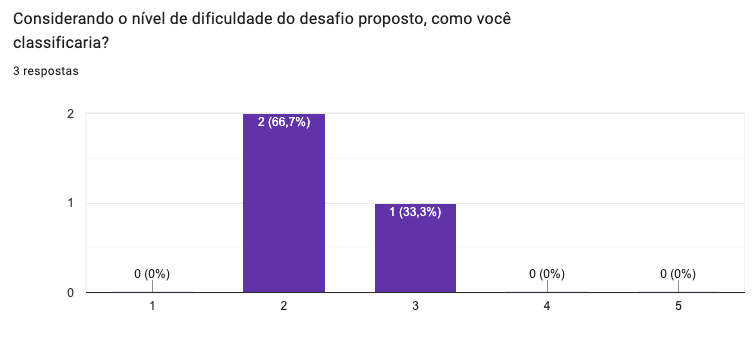
\includegraphics[width=0.95\textwidth]{images/resposta3_com_ia.png}}
        \fonte{Elaborado pelo autor}
    \end{minipage}
\end{figure}
\FloatBarrier

\begin{figure}[ht]
    \caption{Respotas da questão 4 de todos do grupo sem IA}
    \label{graf:resposta4_sem_ia}
    \centering
    \footnotesize
    \begin{minipage}{.9\textwidth}
        \centering
        \fbox{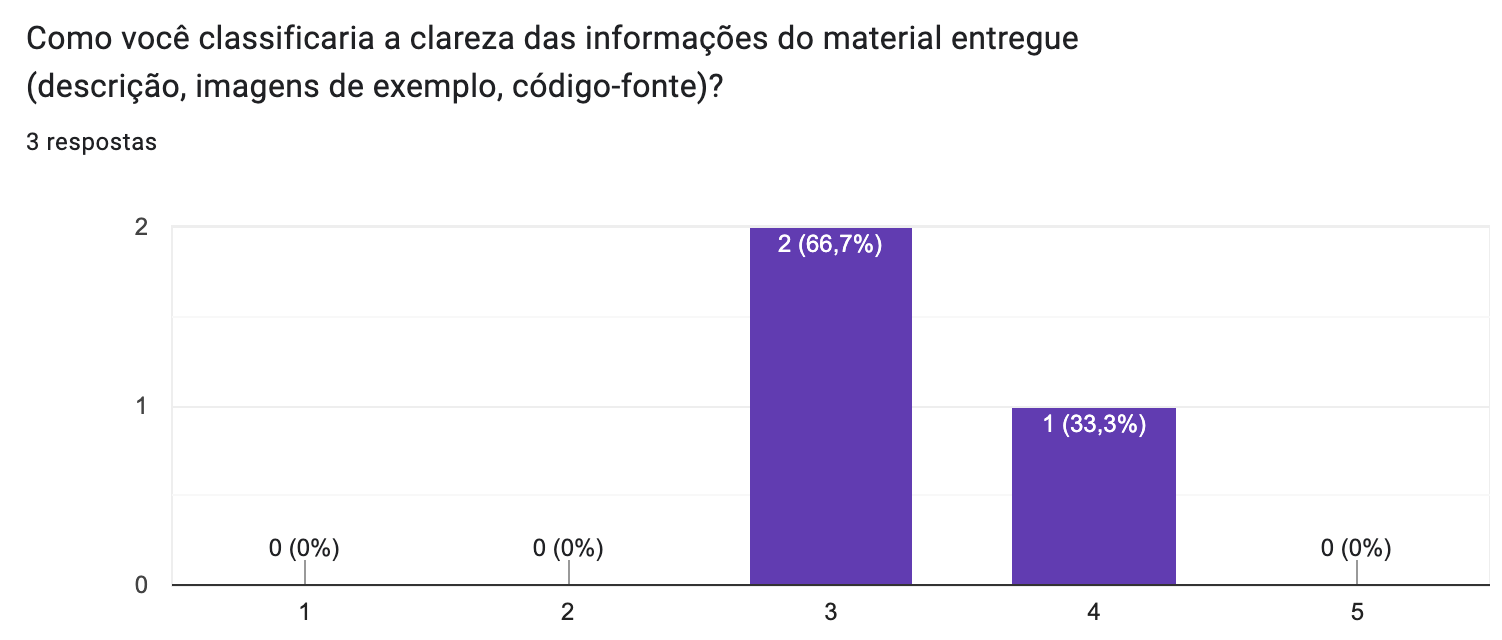
\includegraphics[width=0.95\textwidth]{images/resposta4_sem_ia.png}}
        \fonte{Elaborado pelo autor}
    \end{minipage}
\end{figure}
\FloatBarrier

\begin{figure}[ht]
    \caption{Respotas da questão 4 de todos do grupo com IA}
    \label{graf:resposta4_com_ia}
    \centering
    \footnotesize
    \begin{minipage}{.9\textwidth}
        \centering
        \fbox{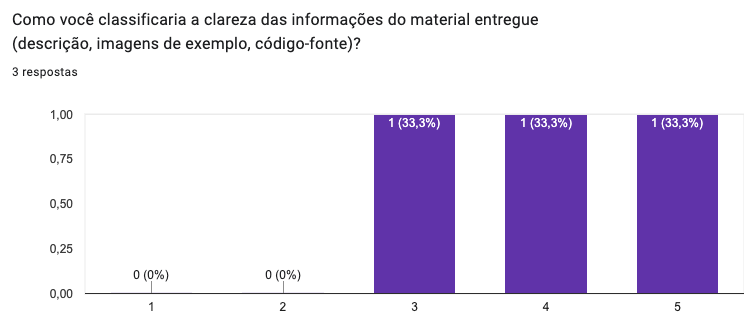
\includegraphics[width=0.95\textwidth]{images/resposta4_com_ia.png}}
        \fonte{Elaborado pelo autor}
    \end{minipage}
\end{figure}
\FloatBarrier

\begin{figure}[ht]
    \caption{Respotas da questão 5 de todos do grupo sem IA}
    \label{graf:resposta5_sem_ia}
    \centering
    \footnotesize
    \begin{minipage}{.9\textwidth}
        \centering
        \fbox{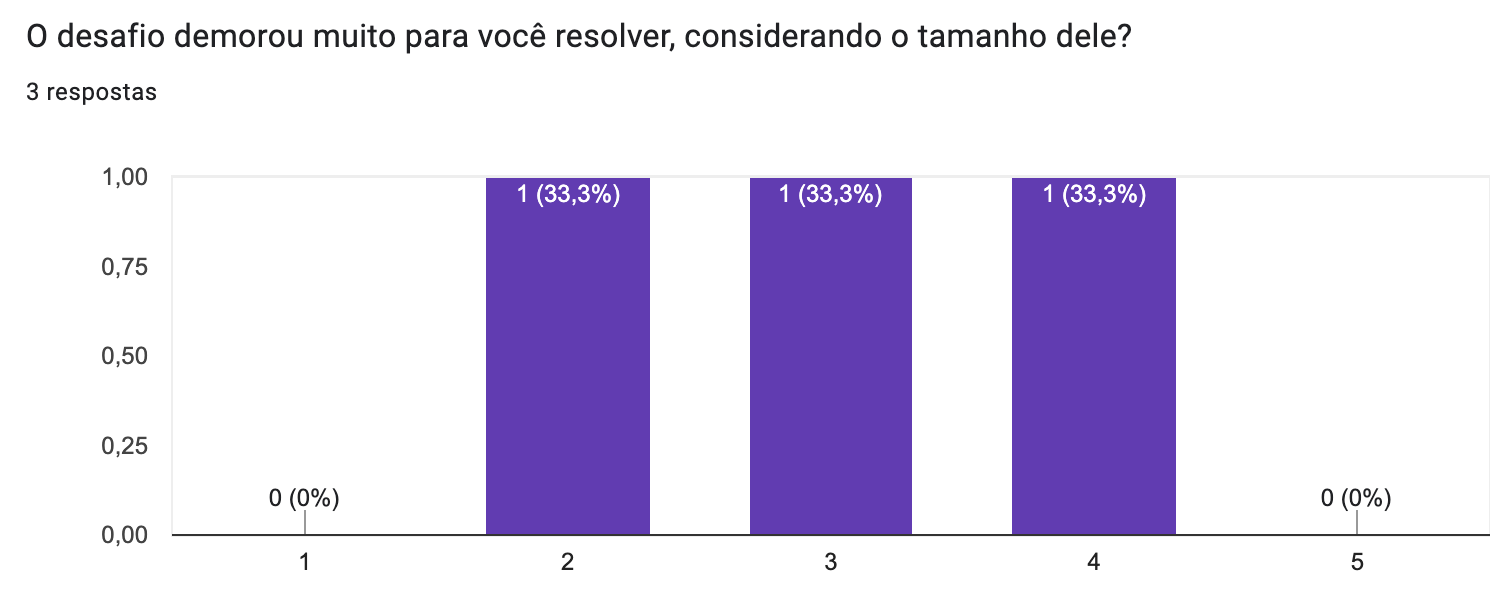
\includegraphics[width=0.95\textwidth]{images/resposta5_sem_ia.png}}
        \fonte{Elaborado pelo autor}
    \end{minipage}
\end{figure}
\FloatBarrier

\begin{figure}[ht]
    \caption{Respotas da questão 5 de todos do grupo com IA}
    \label{graf:resposta5_com_ia}
    \centering
    \footnotesize
    \begin{minipage}{.9\textwidth}
        \centering
        \fbox{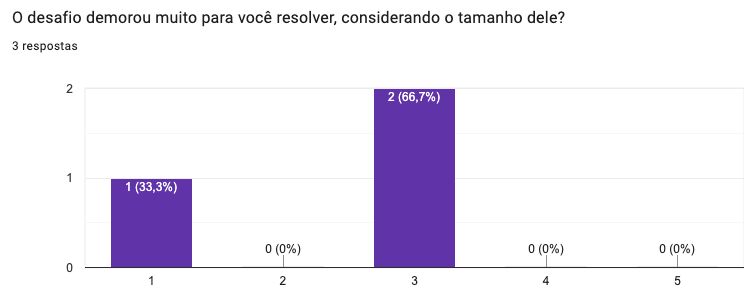
\includegraphics[width=0.95\textwidth]{images/resposta5_com_ia.png}}
        \fonte{Elaborado pelo autor}
    \end{minipage}
\end{figure}
\FloatBarrier

\begin{figure}[ht]
    \caption{Respotas da questão 6 de todos do grupo sem IA}
    \label{graf:resposta6_sem_ia}
    \centering
    \footnotesize
    \begin{minipage}{.9\textwidth}
        \centering
        \fbox{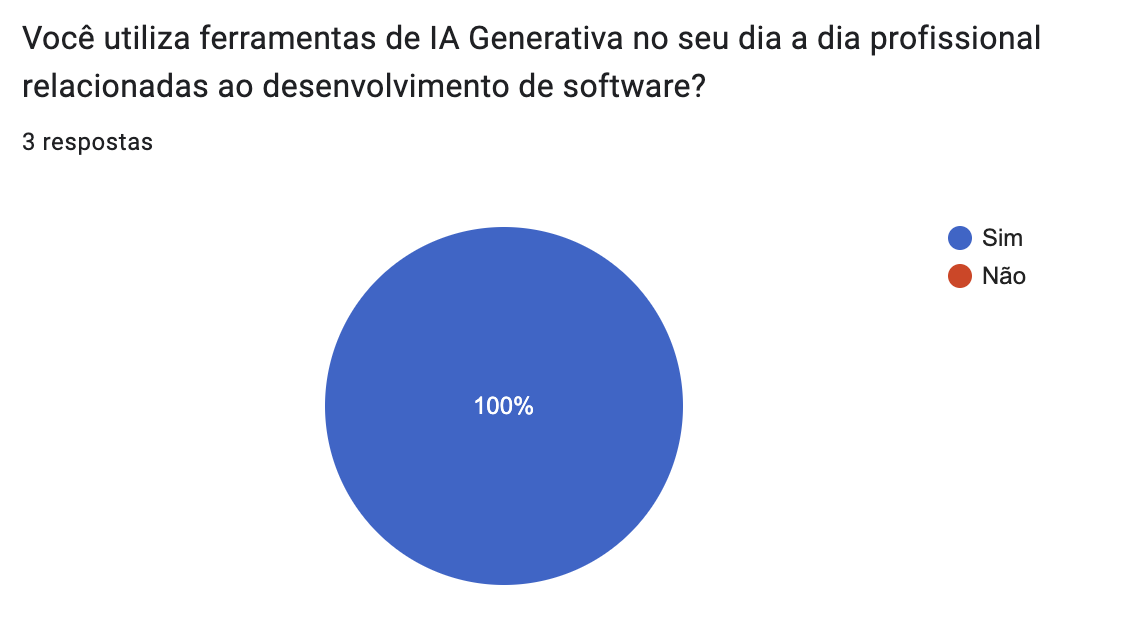
\includegraphics[width=0.95\textwidth]{images/resposta6_sem_com_ia.png}}
        \fonte{Elaborado pelo autor}
    \end{minipage}
\end{figure}
\FloatBarrier

\begin{figure}[ht]
    \caption{Respotas da questão 6 de todos do grupo com IA}
    \label{graf:resposta6_com_ia}
    \centering
    \footnotesize
    \begin{minipage}{.9\textwidth}
        \centering
        \fbox{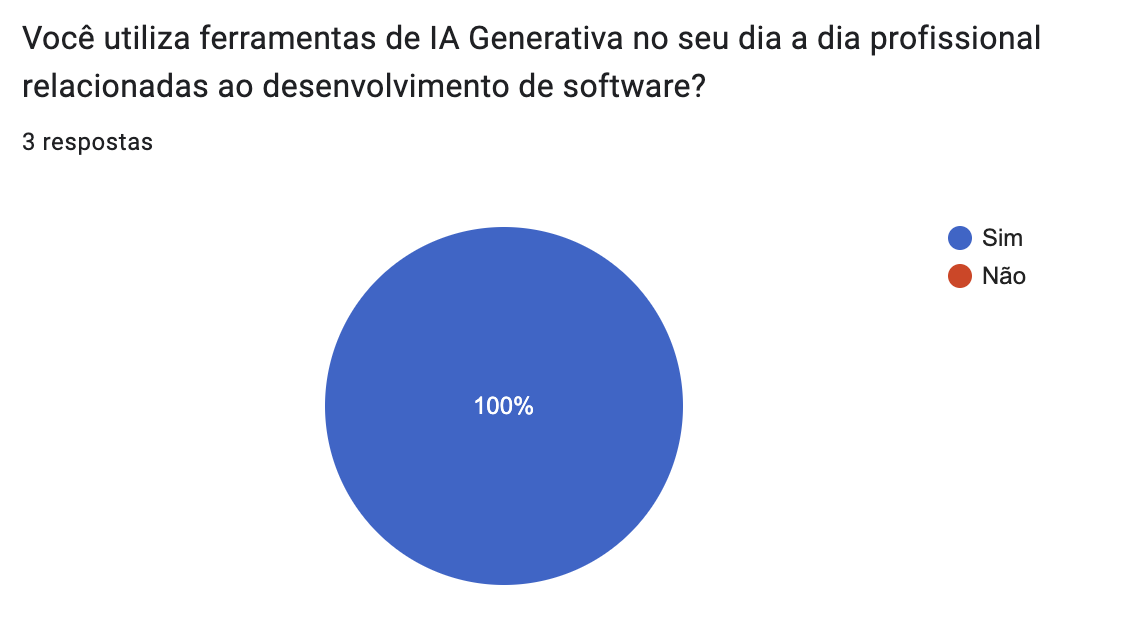
\includegraphics[width=0.95\textwidth]{images/resposta6_sem_com_ia.png}}
        \fonte{Elaborado pelo autor}
    \end{minipage}
\end{figure}
\FloatBarrier

\begin{figure}[ht]
    \caption{Respotas da questão 7 de todos do grupo sem IA}
    \label{graf:resposta7_sem_ia}
    \centering
    \footnotesize
    \begin{minipage}{.9\textwidth}
        \centering
        \fbox{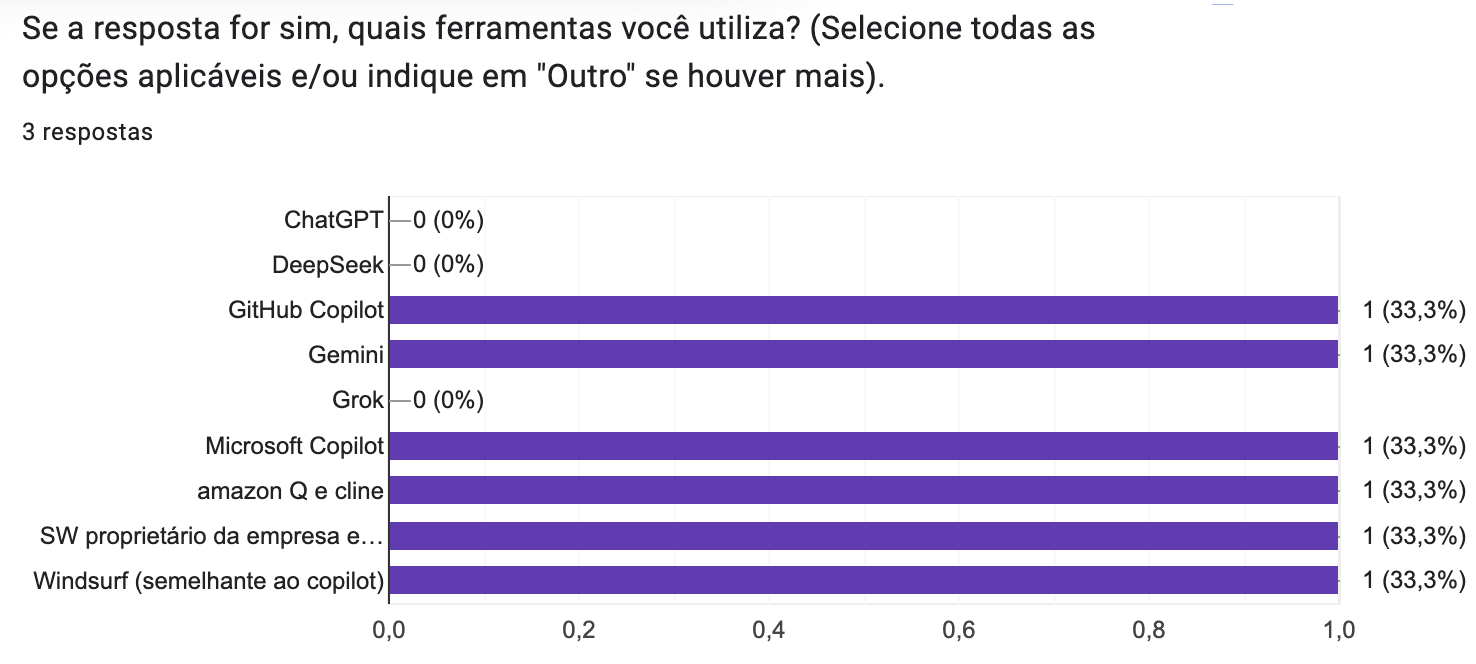
\includegraphics[width=0.95\textwidth]{images/resposta7_sem_ia.png}}
        \fonte{Elaborado pelo autor}
    \end{minipage}
\end{figure}
\FloatBarrier

\begin{figure}[ht]
    \caption{Respotas da questão 7 de todos do grupo com IA}
    \label{graf:resposta7_com_ia}
    \centering
    \footnotesize
    \begin{minipage}{.9\textwidth}
        \centering
        \fbox{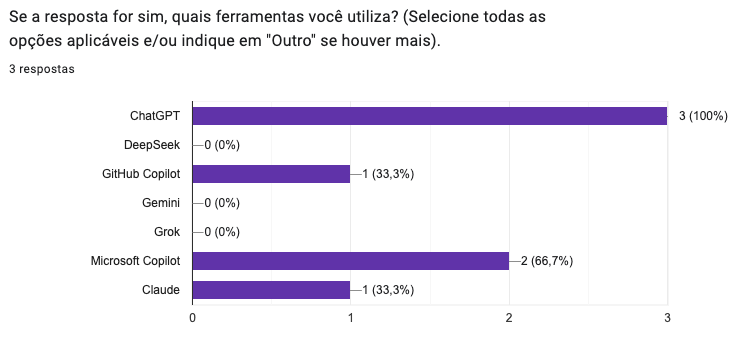
\includegraphics[width=0.95\textwidth]{images/resposta7_com_ia.png}}
        \fonte{Elaborado pelo autor}
    \end{minipage}
\end{figure}
\FloatBarrier

\begin{figure}[ht]
    \caption{Respotas da questão 8 de todos do grupo sem IA}
    \label{graf:resposta8_sem_ia}
    \centering
    \footnotesize
    \begin{minipage}{.9\textwidth}
        \centering
        \fbox{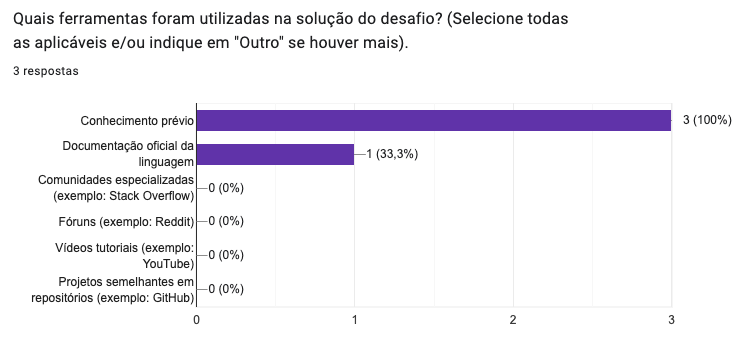
\includegraphics[width=0.95\textwidth]{images/resposta8_sem_ia.png}}
        \fonte{Elaborado pelo autor}
    \end{minipage}
\end{figure}
\FloatBarrier

\begin{figure}[ht]
    \caption{Respotas da questão 8 de todos do grupo com IA}
    \label{graf:resposta8_com_ia}
    \centering
    \footnotesize
    \begin{minipage}{.9\textwidth}
        \centering
        \fbox{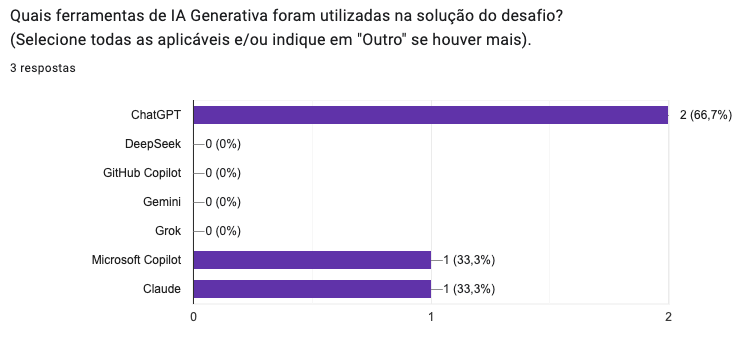
\includegraphics[width=0.95\textwidth]{images/resposta8_com_ia.png}}
        \fonte{Elaborado pelo autor}
    \end{minipage}
\end{figure}
\FloatBarrier

\begin{table}[ht]
    \caption{Respostas da questão 9 de todos do grupo sem IA}
    \label{tab:questao9_sem_ia}
    \centering%
    \footnotesize
    \begin{tabularx}{\textwidth}{lXXXX}
        \toprule
        \textbf{Participante} & \textbf{Em poucas palavras, como você abordou a solução do desafio sem usar ferramentas de IA Generativa?} \\
        \midrule
        Desenvolvedor 1 & Primeiramente, tentei achar os bugs. Para isso, explorei a aplicação já pronta. Tendo isso em vista, fui encontrando a raiz dos problemas e resolvendo. Usei o debugger do navegador para entender quais os problemas com os dados. \\
        \midrule
        Desenvolvedor 2 & Realizei alguns testes e verifiquei o resultado final. A partir daí analisei o código e ajustei conforme fui debugando. \\
        \midrule
        Desenvolvedor 3 & Fui analisando os resultados e revisando o código no VSCode conforme eu encontrava os erros neles \\
        \bottomrule
    \end{tabularx}
    \fonte{Elaborado pelo autor}
\end{table}
\FloatBarrier

\begin{table}[ht]
    \caption{Respostas da questão 9 de todos do grupo com IA}
    \label{tab:questao9_com_ia}
    \centering%
    \footnotesize
    \begin{tabularx}{\textwidth}{lXXXX}
        \toprule
        \textbf{Participante} & \textbf{Em poucas palavras, como você abordou a solução do desafio sem usar ferramentas de IA Generativa?} \\
        \midrule
        Desenvolvedor 4 & Basicamente copiou os prints de output esperados e a descrição do desafio. \\
        \midrule
        Desenvolvedor 5 & Me fiz de leigo. Mandei a IA ler todo o projeto, onde ela ja encontrou e corrigiu bugs, e depois mandei o deafio e pedi pra ele ajustar o projeto de acordo. No final, pedi pra ele testar e me mandar evidencias que está correto. No final, fiz testes exploratorios manuais e entreguei o projeto. \\
        \midrule
        Desenvolvedor 6 & De início eu tentei fazer tudo sozinho, baseado na leitura do código e outputs do programa. Mas, depois de acreditar ter resolvido tudo e ainda assim ver alguns bugs, submeti o código inteiro ao chatGPT, que prontamente já me sugeriu alguns fixes antes de eu pedir qualquer coisa.

        Após isso, somente um bug sobrou, onde agora submeti o input e falei "o resultado atual está errado", e ele prontamente me deu os fixes novamente. \\
        \bottomrule
    \end{tabularx}
    \fonte{Elaborado pelo autor}
\end{table}
\FloatBarrier

\begin{table}[ht]
    \caption{Respostas da questão 10 de todos do grupo sem IA}
    \label{tab:questao10_sem_ia}
    \centering%
    \footnotesize
    \begin{tabularx}{\textwidth}{lXXXX}
        \toprule
        \textbf{Participante} & \textbf{Como integrante do grupo que resolveu o desafio sem IA Generativa, quais obstáculos (se houveram) você enfrentou? Descreva em poucas palavras.} \\
        \midrule
        Desenvolvedor 1 & Encontrar os bugs em si. \\
        \midrule
        Desenvolvedor 2 & Senti falta do autocomplete fornecido pelo windsurf, já que utilizo bastante para tarefas mais manuais. \\
        \midrule
        Desenvolvedor 3 & A pesquisa por informações e a revisão de código tornam-se muito mais demoradas e complicadas sem o uso de IA. \\
        \bottomrule
    \end{tabularx}
    \fonte{Elaborado pelo autor}
\end{table}
\FloatBarrier

\begin{table}[ht]
    \caption{Respostas da questão 10 de todos do grupo com IA}
    \label{tab:questao10_com_ia}
    \centering%
    \footnotesize
    \begin{tabularx}{\textwidth}{lXXXX}
        \toprule
        \textbf{Participante} & \textbf{Como integrante do grupo que resolveu o desafio com IA Generativa, quais obstáculos (se houveram) você enfrentou? Descreva em poucas palavras.} \\
        \midrule
        Desenvolvedor 4 & chatgpt free, tem um limite muito pequeno de entradas, tive que ir para o Copilot \\
        \midrule
        Desenvolvedor 5 & Nenhum. \\
        \midrule
        Desenvolvedor 6 & Com IA, nenhum. \\
        \bottomrule
    \end{tabularx}
    \fonte{Elaborado pelo autor}
\end{table}
\FloatBarrier

\begin{table}[ht]
    \caption{Respostas da questão 11 de todos do grupo sem IA}
    \label{tab:questao11_sem_ia}
    \centering%
    \footnotesize
    \begin{tabularx}{\textwidth}{lXXXX}
        \toprule
        \textbf{Participante} & \textbf{Algum feedback adicional que gostaria de compartilhar referente ao experimento?} \\
        \midrule
        Desenvolvedor 2 & Faltou ser um pouco mais claro na descrição do problema \\
        \midrule
        Desenvolvedor 3 & Interessante notar como a IA se tornou uma ferramenta tão importante no meu processo de desenvolvimento. Antes do experimente eu poderia dizer que fácilmente conseguiria desenvolver sem o uso de IA mas após ele consigo notar que o processo se torna muito mais demorado sem o uso da mesma. \\
        \bottomrule
    \end{tabularx}
    \fonte{Elaborado pelo autor}
\end{table}
\FloatBarrier

\begin{table}[ht]
    \caption{Respostas da questão 11 de todos do grupo com IA}
    \label{tab:questao11_com_ia}
    \centering%
    \footnotesize
    \begin{tabularx}{\textwidth}{lXXXX}
        \toprule
        \textbf{Participante} & \textbf{Algum feedback adicional que gostaria de compartilhar referente ao experimento?} \\
        \midrule
        Desenvolvedor 6 & seria muito mais simples se nas instruções não houvessem prints da tela, mas sim textos de input e output, pra que a gente copiasse e colasse, invés de ter que ler a imagem e copiar. \\
        \bottomrule
    \end{tabularx}
    \fonte{Elaborado pelo autor}
\end{table}
\FloatBarrier

\section{CÓDIGO-FONTE BASE E CÓDIGO-FONTE DO DESAFIO}

\renewcommand{\thelstlisting}{G.\arabic{lstlisting}}

\lstinputlisting[caption={Código-fonte base do Desafio Técnico}]{source_code/main_base.js}

\lstinputlisting[caption={Código-fonte do Desafio Técnico}]{source_code/main.js}

\section{LISTA DE \textit{BUGS} E ANÁLISES DOS DESENVOLVEDORES}

\renewcommand{\thefigure}{H.\arabic{figure}}
\setcounter{figure}{0}

\begin{figure}[ht]
    \caption{Lista de \textit{bugs} implementados no arquivo \texttt{main.js}}
    \label{fig:bugs}
    \centering
    \footnotesize
    \begin{minipage}{.9\textwidth}
        \centering
        \fbox{\includegraphics[width=1\textwidth]{images/bugs.png}}
        \fonte{Elaborado pelo autor}
    \end{minipage}
\end{figure}
\FloatBarrier

\begin{figure}[ht]
    \caption{Análises dos desenvolvedores do grupo sem IA}
    \label{fig:resultados_bugs_sem_ia}
    \centering
    \footnotesize
    \begin{minipage}{.9\textwidth}
        \centering
        \fbox{\includegraphics[width=1\textwidth]{images/resultados_bugs_sem_ia.png}}
        \fonte{Elaborado pelo autor}
    \end{minipage}
\end{figure}
\FloatBarrier

\begin{figure}[ht]
    \caption{Análises dos desenvolvedores do grupo com IA}
    \label{fig:resultados_bugs_com_ia}
    \centering
    \footnotesize
    \begin{minipage}{.9\textwidth}
        \centering
        \fbox{\includegraphics[width=1\textwidth]{images/resultados_bugs_com_ia.png}}
        \fonte{Elaborado pelo autor}
    \end{minipage}
\end{figure}
\FloatBarrier

\end{document}
